\def\year{2018}\relax
%File: formatting-instruction.tex
\documentclass[letterpaper]{article} %DO NOT CHANGE THIS
\usepackage{aaai18}  %Required
\usepackage{times}  %Required
\usepackage{helvet}  %Required
\usepackage{courier}  %Required
\usepackage{url}  %Required
\usepackage{graphicx}  %Required
\usepackage{enumitem}
\usepackage{lipsum}
\setlist[enumerate]{itemsep=0mm}
\frenchspacing  %Required
\setlength{\pdfpagewidth}{8.5in}  %Required
\setlength{\pdfpageheight}{11in}  %Required
%PDF Info Is Required:
\pdfinfo{
	/Title (Transfer Learning for Traffic Speed Prediction: A Prelininary Study)
	/Author (Bill Y. Lin, Frank F. Xu, Eve Q. Liao, Kenny Q. Zhu)}

\title{Transfer Learning for Traffic Speed Prediction: A Preliminary Study}

% The \author macro works with any number of authors. There are two
% commands used to separate the names and addresses of multiple
% authors: \And and \AND.
%
% Using \And between authors leaves it to LaTeX to determine where to
% break the lines. Using \AND forces a line break at that point. So,
% if LaTeX puts 3 of 4 authors names on the first line, and the last
% on the second line, try using \AND instead of \And before the third
% author name.
\author{
	Bill Y. Lin\thanks{The first two authors contribute equally.}, ~
	Frank F. Xu\footnotemark[1], ~ Eve Q. Liao,~
	Kenny Q. Zhu
	\\[0.5ex]
	{\{yuchenlin, frankxu, liaoqz\}@sjtu.edu.cn, kzhu@cs.sjtu.edu.cn}\\[0.5ex]
	Department of Computer Science and Engineering\\[0.5ex]
	Shanghai Jiao Tong University, Shanghai, China
}

\usepackage{amsmath,amsfonts,amsthm}
\usepackage{color}
\usepackage{array}
\usepackage{epsfig}
\usepackage{caption}
\usepackage{subcaption}
\usepackage{array}
\usepackage{ragged2e}
\usepackage{pbox}

\usepackage[ruled,vlined,boxed,linesnumbered]{algorithm2e}
\SetAlFnt{\small}
\SetAlCapFnt{\small}
\SetAlCapNameFnt{\small}
\usepackage{float}
\restylefloat{table}
\newcolumntype{P}[1]{>{\RaggedRight\hspace{0pt}}p{#1}}
\newcolumntype{L}[1]{>{\raggedright\let\newline\\\arraybackslash\hspace{0pt}}m{#1}}
\newcolumntype{C}[1]{>{\centering\let\newline\\\arraybackslash\hspace{0pt}}m{#1}}
\newcolumntype{R}[1]{>{\raggedleft\let\newline\\\arraybackslash\hspace{0pt}}m{#1}}


\newcommand{\secref}[1]{Section \ref{#1}}
\newcommand{\figref}[1]{Figure \ref{#1}}
\newcommand{\eqnref}[1]{Eq. (\ref{#1})}
\newcommand{\tabref}[1]{Table \ref{#1}}
\newcommand{\exref}[1]{Example \ref{#1}}
\newcommand{\algref}[1]{Algorithm \ref{#1}}
\newcommand{\socvec}{SocVec}
\newcommand{\argmin}{\operatornamewithlimits{argmin}}
\newcommand{\argmax}{\operatornamewithlimits{argmax}}
\newtheorem{example}{Example}
\newtheorem{lemma}{Lemma}
\newtheorem{definition}{Definition}
\newcommand{\cut}[1]{}
\newcommand{\li}{\uline{\hspace{0.5em}}}
\newcommand{\BL}[1]{\textcolor{blue}{Bill: #1}}
\newcommand{\HY}[1]{\textcolor{red}{Hanyuan: #1}}
\newcommand{\KZ}[1]{\textcolor{green}{Kenny: #1}}
\newcommand{\SH}[1]{\textcolor{green}{Seung: #1}}
\newcommand{\FX}[1]{\textcolor{blue}{Frank: #1}}


%\author{
%  David S.~Hippocampus\thanks{Use footnote for providing further
%    information about author (webpage, alternative
%    address)---\emph{not} for acknowledging funding agencies.} \\
%  Department of Computer Science\\
%  Cranberry-Lemon University\\
%  Pittsburgh, PA 15213 \\
%  \texttt{hippo@cs.cranberry-lemon.edu} \\
  %% examples of more authors
  %% \And
  %% Coauthor \\
  %% Affiliation \\
  %% Address \\
  %% \texttt{email} \\
  %% \AND
  %% Coauthor \\
  %% Affiliation \\
  %% Address \\
  %% \texttt{email} \\
  %% \And
  %% Coauthor \\
  %% Affiliation \\
  %% Address \\
  %% \texttt{email} \\
  %% \And
  %% Coauthor \\
  %% Affiliation \\
  %% Address \\
  %% \texttt{email} \\
%}

\begin{document}
% \nipsfinalcopy is no longer used

\maketitle

\begin{abstract}
Traffic speed prediction can benefit a wide range of IoT applications in intelligent transportation and smart city. 
%including travel time forecasting, vehicle navigation devices, vehicle routing, congestion management and urban planning.
Recent supervised machine learning approaches heavily leverage vast amount of historical time-series data. 
Consequently, they degrade dramatically in the areas where collecting a large traffic data is not quite feasible.
With the aim of predicting the traffic speed of such urban areas, 
we propose a transfer learning framework that exploits historical data of some other data-abundant areas by utilizing various spatio-temporal semantic features. 
Experimental results show that classic regression models and our proposed kernel regression model can achieve competitive performance comparing to baseline methods that heavily rely on the historical data of target areas.
\end{abstract}
%\IEEEraisesectionheading{
% %\IEEEraisesectionheading{
% %\IEEEraisesectionheading{
% \input{intro}
\section{Introduction}\label{sec:intro}
 %}
% \section{Introduction}\label{sec:intro}

% \begin{enumerate}
% \item Motivation: application scenarios (with 1-2 running examples);
% \item Characteristics of the data sources and their challenges;
% \item Briefly introduce previous approaches to extract information 
% from images including setting the document zone, and their limitations.
% \item General flow of our approach (may give a diagram here)
% \end{enumerate}
% scenary

Due to ever evolving hardware and software, many medical images
such as electro-cardio graphs (ECGs), X-ray or ultrasound images  
are directly printed and stored in hard copy formats. 
% \KZ{Insert 4 example images here.}
%Examples are shown in \figref{fig:medicalImages}. 
% These images often contain a mix of graphics and text, which
% include parameter settings of the hardware, test measurements or simple
% diagnosis. 
These images often contain a mix of graphics and text, which 
include technical settings of the hardware used, test measurements or simple diagnoses.
Recently, there has been a growing demand for digitizing such 
medical information from paper media sources, especially legacy ones, or patients who want to keep track of these documents by themselves digitally. 
Apart from scanning the graphics into a digital format, extracting 
the semi-structured textual information is also an important part of
building electronic medical records for patients. 

%\begin{figure}[!htb]
%\centering
%\subfloat[ECG]{
%\label{fig:medicalimage:ecg}
%\epsfig{file=figure/17_ori.eps, width=0.4\columnwidth}
%}
%% \hfill
%\subfloat[MRI]{
%	\label{fig:medicalimage:mrt}
%	\epsfig{file=figure/MRI.eps, width=0.4\columnwidth}
%}
%\\
%\subfloat[X-RAY]{
%\label{fig:medicalimage:xray}
%\epsfig{file=figure/X-RAY.eps, width=0.4\columnwidth}
%}
%%\hfill
%\subfloat[EEG]{
%\label{fig:medicalimage:eeg}
%\epsfig{file=figure/EEG.eps, width=0.4\columnwidth}
%}
%\caption{Examples of Medical Images}
%\label{fig:medicalImages}
%\end{figure}

Optical character recognition (OCR)  \cite{mori1992historical,smith2007overview} is 
a traditional technique used to turn images of printed text into machine encoded
text. It is well researched and performs well on plain text 
documents such as novels and reports, for a variety of languages. 
%For example, Tesseract, which is one of 
%the most popular open source multilingual recognizers, logs an error 
%rate of 3.72\% for English words and 3.77\% for simplified 
%Chinese characters\cite{smith2009adapting}. 
%Google Books \cite{googlebooks} and Gutenberg \cite{gutenberg} are
%projects which have scanned a large number of paper books into text for free and open
%access. These projects made exclusive use of OCR for this conversion and 
%achieved high accuracy \cite{vincent2007google} \cite{lebert2008project}. 
% 99\% for Gutenberg project \cite{lebert2008project}. 
% \KZ{Give the accuracy of google and gutenberg if available.}


\begin{figure}[th]
\centering
\epsfig{file=figure/17_b.eps, width=0.8\columnwidth}
\caption{An ECG image with text area (red circle) of interest.}
\label{fig:ecgexample2}
\end{figure}

For a semi-structured medical image, such as 
\figref{fig:ecgexample2}, we would like to extract the attribute-value 
pairs (e.g., {\em Vent. rate = 63 bpm}) and possibly other values such as
date ({\em 18-Nov-2010}) and time ({\em 9:13:02}) since those values endow us with lots of information about the patient. 
Existing OCR software cannot extract such structured information in a straightforward 
fashion, 
but instead it produces rather convoluted results from the whole image, 
similar to those in \figref{fig:ocrre}, which was produced by Tesseract, 
a popular multi-lingual recognizers. 
% \KZ{Maybe include the x-y coordinate info in the output as well?}  

\begin{figure}[th]
\centering
\scriptsize
\begin{verbatim}
<p class="ocr_par" title="box 263 33 444 119">
   <span class="ocr_l" title="box 264 33 336 45">
       <span class="ocrx_w" title="box 264 33 299 45">Vcnt.</span> 
       <span class="ocrx_w" title="box 308 34 336 45">rule</span> 
   </span>
   <span class='ocr_l'>
       <span class="ocrx_w" title="box 264 51 283 64">PR</span> 
       <span class="ocrx_w" title="box 291 51 346 64">Interval</span> 
       <span class="ocrx_w" title="box 389 52 411 64">140</span> 
       <span class="ocrx_w" title="box 420 55 439 64">ms</span> 
   </span>
   ...
   </span>
</p>
<p class="ocr_p" dir="ltr">
   <span class="ocr_l">
       <span class="ocrx_w" title="box 396 33 411 45">53</span> 
       <span class="ocrx_w" title="box 420 33 449 48">bpm</span> 
   </span>
</p>
\end{verbatim}
\caption{Snippet OCR results in XML, input to our framework.}
\label{fig:ocrre}
\end{figure}


%\input{xmlre1}

%However, OCR alone does not work well on semi-structured text and hence
%can't be directly used for information extraction from the aforementioned
%medical images. \KZ{Give the reason here, perhaps because OCR models are
%largely Markov based? So semi-structured data breaks the flow of text.}
%When a medical image is input to an ordinary OCR software, the spatial 
%information of the text components is often lost or mixed with noises
%and errors.
%%The reason is OCR converts the whole images into text data, in which 
%%useful information often mix with noises and errors. 
%In this paper, we would like to extract the attribute-value pairs
%and possibly other values from \figref{fig:ecgexample1} 
%and \figref{fig:ecgexample2}. 
%% or medical ultrasonography report. 
%Such images contain lots of non-textual information or noises.

% example & ref
%\begin{figure}[ht]
%\centering
%\epsfig{file=figure/46.eps, width=0.8\columnwidth}
%\caption{ECG Images From Printer1}
%\label{fig:ecgexample1}
%\end{figure}

% \begin{figure}[ht]
% \centering
% \subfloat[Printer1]{
% \label{fig:ecgexample:a}
% \epsfig{file=figure/46.eps, width=0.48\columnwidth}
% }
% \hfill
% \subfloat[Printer2]{
% \label{fig:ecgexample:b}
% \epsfig{file=figure/17.eps, width=0.48\columnwidth}
% }
% \caption{ECG images from two different printers}
% \label{fig:ecgexample}
% \end{figure}

Also, errors in the OCR text \cite{darwish2007error,taghva1996evaluation} will greatly affect the effectiveness 
of other related tasks. Much work has been done to improve the performance of the OCR\cite{kolak2003generative,cesarini1998informys}. However, there are still a number of significant challenges involved in extracting the information from medical images or OCR results in XML form. 

% First, medical images differ from pure text document in that them have 
% layout information. 
First, medical images differ from pure text documents in that 
they contain layout information.
Although most current OCR engines attempt to reproduce the physical 
layout of the text units, 
%(along with X-Y coordinates) and store them 
%in a special format such as XML 
% (\KZ{Better in the previous example})
such spatial
information is approximate and sometimes inaccurate, which is why neighboring
text blocks in \figref{fig:ecgexample2}, such as ``Vent. Rate'' and
``63 bpm'' were not automatically combined into the same XML block, but were 
rather far apart (shown in two different ``classes'') in \figref{fig:ocrre} made by OCR softwares. 
%Even for images produced by the same ECG printer, 
%the XML results can still be very different as 
The spatial layout is sensitive to many factors, such as accidental spots 
on the prints, color and contrast, or the angle of the camera. 
%In this case, solutions for other application domains, for example, the web, 
%are not well suited for information extraction from printed documents \cite{bartoli2014semisupervised}. With such inaccurate
%layout information produced by OCR,
%it is not easy to write a simple wrapper program to extract useful
%data from images, even if the images come from the same printer. 

%Writing a wrapper for each
%individual image would be tedious and counter-productive. Therefore,
%a mechanism that makes use of the spatial locality of the 
%text units in the image and 
%accommodates slight variations in the spatial layout would make the extraction
%more accurate and fault-tolerant.

%For example, \figref{fig:ocrre} is the simplified OCR results for the ECGs in 
%\figref{fig:ecgexample1} and \figref{fig:ecgexample2}. The results are in the XML format and have attritube named {\em class} 
%for layout information. Although these two images share similar format. 
%OCR engine generates different results in that it splits elements that 
%should be in the same line into two lines in the second example. 
%XML is sensitive to the layout results so it's hard to tolerate 
%all the layout results. 
%
% example check the term
% layout of ocr results can be restore, so why OCR engine don't restore the results 
% using the similar methods as we do?
% or the way we handle the layout problem is quite simple

% Delete for TIP
% Second, exiting OCR engines make heavy use of Markov properties such as n-grams
% since they primarily target the transformation of large body of text 
% \cite{kolak2003generative}. 
% % \KZ{Needs some refs here.}
% Unfortunately, the semi-structured texts in medical images are often 
% short and not even written in complete sentences, thus breaking Markov assumption. To make
% matters worse, medical images contain scientific language, which may be
% very different from the training corpora of these OCR engines.
% This explains why we see errors like ``Vcnt'' and ``rule'' 
% in \figref{fig:ocrre}. 
% %can't guarantee a perfect performance, which means 
% %there are errors and noises in the OCR results.
% %Many of them due to the fact that the data are no longer long, continous
% %sentences, thus breaking the Markov assumption made by many OCR algorithms. 
% %In \figref{fig:ocrresub:b}, ``Vent." is misrecognized as ``Vcnt.". 
% Without sufficient contextual information, OCR may also misrecognize a 
% digit as an alphabetic character, or as another similar digit. 
% Furthermore, the mix of text with images and formatting
% lines often confuses the OCR engine, which is more biased toward full
% text images.
% Exact pattern matching, as used in
% traditional information extraction, doesn't work with such noisy OCR output
% as it doesn't tolerate noises or errors in text. 
% %It's hard to autocorrect these errors 
% %because image quality is the most important affecting factor. 
% %The text we are processing can be full of no meaning words or 
% %strange numbers. 
% A fuzzy matching strategy is more desirable in this case. 
% % example, what are the traditional IEs

Second, there are many types of medical images, resulting from a variety of
medical tests. Different equipments for the same test can produce vastly 
different images. Writing individual extraction wrappers 
for the OCR outputs of all these formats is tedious and inefficient, 
and difficult for non-programmers.
%not to mention that there are significant programming barriers for 
%writing these wrappers, especially for the medical professionals who are the
%end users of these extraction results. 
%A more user-friendly approach enabling users to specify such extraction requirements would be preferred. 
%There are various kinds of medical images, such as electrocardiograph report, 
%medical ultrasonography report, etc. 
%However the basic measures for each type of medical test (e.g., ECG), 
%are very similar from machine to machine. Only the layouts are 
%different. 
% example medical images

Finally, most off-the-shelf OCR programs are pre-trained with specific 
recognition models, which may not be suitable for the extraction of 
%medical images.
%Furthermore, changes in imaging equipment technology over time may produce 
%different formats, layout, or terminology, rendering existing OCR models 
%obsolete. 
Re-training the models requires a large amount of labeled data, which may
not be available. 
%Incremental training as more labeled data arrives
%is currently not supported by any OCR product.    

%There have been some limited attempts to address some of the above challenges. 
%One solution is a plugin of an OCR program that allows the user to specify 
%target zones of interest in the image to be extracted. The zones specified for
%one image can be applied to images with slight variations by adjusting against
%a fixed reference point that is supposed to exist in all these images.
%% \KZ{I think the problem is not so much with the zones, because we also
%% have zones, but rather with the reference point.}
%% \JY{}
%% example products
%% http://www.square-9.com/automated-data-extraction-optical-character-recognition
%The problem with this solution is its high reliance on the OCR zones  
%established by the user. The performance of the results is affected by the 
%accuracy of the zones. If the zones are too big, the results will be full of 
%noise. If the zones are too small, results will miss something. 
%
%Another solution involves using the page layout analysis technique. The page layout 
%analysis technique is used to determine where the text 
%resides on a page \cite{o1993document}, 
%% \KZ{This page layout analysis approach is not clearly described. I don't understand after reading this paragraph.}
%% By using page layout analysis technique, the hierarchy of physical components 
%% can be generated and to match with the hierarchy of logical components, which 
%% is predefined. 
%this includes identifying and categorizing the 
%regions of interest in the scanned image of a text document. 
%Typically, the first step is to segment text zones from 
%non-textual zones and arrange them in their original order. 
%Then in order to analyze the logical roles of the text zones 
%(titles, captions, footnotes, etc.), logical layout analysis 
%is used for labeling the semantics of the text zones.
%Generally, page layout analysis is used for documents. The problem with applying 
%such a technique on medical images is that it creates so much noises 
%that performance is ultimately affected. 
%For medical imaging reports like ECG, useful information is often 
%found in the small components of the image, while most of the images are 
%read as noises. 
% check paper and more description, weakness, ref

%In this paper, 
%we propose a spatial data description language, which borrows its syntax from
%PADS \cite{fisher+:pads}, an ad hoc data processing language, 
%for describing semi-structured data in medical images. 
%% ref
%We call this language OCR description language, or ODL. 
%ODL is designed for extracting and parsing semi-structured text data 
%from images. We believe that  information extraction from those data in ODL form may be much easier than extracting information from rough data or data in XML form, which means that our preprocessing part proves to be necessary.
%%An example ODL description for the image in 
%%\figref{fig:ecgexample2} is shown in 
%%\figref{fig:description}. \KZ{Make this description two column, and give
%%some brief explanation of this description here.} 
%%The parsing result of this description is shown
%%in \figref{fig:parsing result}. \KZ{Give some explanation of the results,
%%otherwise don't show the result here. E.g., you need to explain what F, E, etc.
%%mean. You want to say that even though rate has been recognized as rule,
%%the bpm value was still extracted (but still wrong!).}
%% \KZ{I removed the preprocessing part, cos it's not important. Talk about it in
%% discussion sec.}
%%The our approach starts by preprocessing the images for text results.
%To use this framework, the user first describes the components in the image
%that he or she is interested in extracting. This includes constant strings
%and variables of different data types.   
%ODL allows the user to specify the approximate spatial layout and constraints on
%the data, e.g., integers within 
%a certain range, real numbers with certain decimal points, etc. 
%%This information is then as the key component in our fuzzy matching strategy. 
%The system then automatically generates a parser for these medical images.
%This parser uses the output XML from OCR with spatial information as an input, 
%and outputs a data structure with values extracted for each variables
%in the description, unless there is an unrecoverable error during the parsing process.
%In addition, approximate layout information and constraints are used in parsing process 
%to tolerate noises and small format variations in the input images. 
%%Specifically, this method could be called fuzzy matching, meaning that more candidates could be saved after the parsing process.  It's obvious that we may have a higher probability to obtain the accurate result if more candidates are kept so that fuzzy match should be used properly in our system.
%%An autogenerated parser based on the ODL description can release us from 
%%repetitive work. In this way, we turn the task of writing complex parsers 
%%into describing information on images.
%
%
%When users process many images of the same format, the system 
%automatically discovers parsing errors given the current model and 
%prompts the user to manually correct some of the frequent and prominent
%errors, which effectively serves as an online labeling function. 
%These incrementally labeled data are then used to update the parsing model. 


%It should be emphasized that the incremental learning model is very important in our whole system. Incremental learning is a machine learning paradigm where the learning process takes place whenever we have new examples or data added to our baisc data set, leading to a most striking difference between incremental learning and traditional machine learning: it does not assume the availability of a sufficient training set before the learning process. What incremental learning in our system is really impressive: it does not require a relatively good and stable training set at first time. In fact, it could improve the parsing result with even relatively rough training sets at first by absorbing new data or corrective information as time passes in dynamic systems. Besides, the process would be very effective when there are some new images coming in since training process would not learn from scratch, which might waste time and computation resource.

%At last, we propose an incrementally human correction framwork which can 
%make the best use of human correction to handle the misrecognition problem. 
% Base on our experiments on about 500 real life ECG images, 
% our approach achieves p1 and p2 after p3 times human correction. 
% experimental results

% \begin{figure}[h]
% \begin{lstlisting}
% Oenum str_month_t{
% 	"Jan", "Feb", "Mar", "Apr",
% 	"May", "Jun", "Jul", "Aug",
% 	"Sept", "Oct", "Nov", "Dec"
% };

% Ounion month_t{
% 	Oint(1,12)	num;
% 	str_month_t	str;
% };

% Ostruct time_t{
% 	Oint(1,31)	day;
% 	"-";
% 	month_t	month;
% 	"-";
% 	Oint	year;
% };

% Ostruct triple_t{
% 	"Vent.";
% 	hskip(\s)	skip1;
% 	"rate";
% 	Oint x;
% 	"bpm";
% 	vskip(\n)	skip2;
% };

% Oscource Ostruct entry_t{
% 	time_t(<-,-,-,0.3l>) t;
% 	triple_t(<0.1w,-,0.5w,->) d;
% };
% \end{lstlisting}
% \caption{Description}\label{fig:description}
% \end{figure}


In order to solve above problems, We design a system which makes three main contributions:
\begin{enumerate}
\item Based on some previous work on data description language \cite{lamport1986document,taft1999post,fisher+:pads},we design a new declarative spatial data description language called \textit{OCR description language}, or ODL,
which allows users to specify spatial and data constraints in medical 
images(\secref{sec:syntax});
\item We propose a noise-tolerant parser which takes OCR results
the ODL description as input and outputs a data structure with values 
extracted for each variables in the description (\secref{sec:semantics});
\item We propose an incremental manual correction 
framework\cite{von2008recaptcha,zhu2012learnpads++}, which 
takes advantage of user corrections  and improves the productivity
significantly (\secref{sec:correction}).
%To be more specific, the framework improves the traditional machine learning methods by using a incremental learning process to avoid starting from scratch when we are trying to apply human corrections in the system. That means the framework would be more effective than most corrective systems.
\end{enumerate}


\section{Introduction}\label{sec:intro}
 %}
% \section{Introduction}\label{sec:intro}

% \begin{enumerate}
% \item Motivation: application scenarios (with 1-2 running examples);
% \item Characteristics of the data sources and their challenges;
% \item Briefly introduce previous approaches to extract information 
% from images including setting the document zone, and their limitations.
% \item General flow of our approach (may give a diagram here)
% \end{enumerate}
% scenary

Due to ever evolving hardware and software, many medical images
such as electro-cardio graphs (ECGs), X-ray or ultrasound images  
are directly printed and stored in hard copy formats. 
% \KZ{Insert 4 example images here.}
%Examples are shown in \figref{fig:medicalImages}. 
% These images often contain a mix of graphics and text, which
% include parameter settings of the hardware, test measurements or simple
% diagnosis. 
These images often contain a mix of graphics and text, which 
include technical settings of the hardware used, test measurements or simple diagnoses.
Recently, there has been a growing demand for digitizing such 
medical information from paper media sources, especially legacy ones, or patients who want to keep track of these documents by themselves digitally. 
Apart from scanning the graphics into a digital format, extracting 
the semi-structured textual information is also an important part of
building electronic medical records for patients. 

%\begin{figure}[!htb]
%\centering
%\subfloat[ECG]{
%\label{fig:medicalimage:ecg}
%\epsfig{file=figure/17_ori.eps, width=0.4\columnwidth}
%}
%% \hfill
%\subfloat[MRI]{
%	\label{fig:medicalimage:mrt}
%	\epsfig{file=figure/MRI.eps, width=0.4\columnwidth}
%}
%\\
%\subfloat[X-RAY]{
%\label{fig:medicalimage:xray}
%\epsfig{file=figure/X-RAY.eps, width=0.4\columnwidth}
%}
%%\hfill
%\subfloat[EEG]{
%\label{fig:medicalimage:eeg}
%\epsfig{file=figure/EEG.eps, width=0.4\columnwidth}
%}
%\caption{Examples of Medical Images}
%\label{fig:medicalImages}
%\end{figure}

Optical character recognition (OCR)  \cite{mori1992historical,smith2007overview} is 
a traditional technique used to turn images of printed text into machine encoded
text. It is well researched and performs well on plain text 
documents such as novels and reports, for a variety of languages. 
%For example, Tesseract, which is one of 
%the most popular open source multilingual recognizers, logs an error 
%rate of 3.72\% for English words and 3.77\% for simplified 
%Chinese characters\cite{smith2009adapting}. 
%Google Books \cite{googlebooks} and Gutenberg \cite{gutenberg} are
%projects which have scanned a large number of paper books into text for free and open
%access. These projects made exclusive use of OCR for this conversion and 
%achieved high accuracy \cite{vincent2007google} \cite{lebert2008project}. 
% 99\% for Gutenberg project \cite{lebert2008project}. 
% \KZ{Give the accuracy of google and gutenberg if available.}


\begin{figure}[th]
\centering
\epsfig{file=figure/17_b.eps, width=0.8\columnwidth}
\caption{An ECG image with text area (red circle) of interest.}
\label{fig:ecgexample2}
\end{figure}

For a semi-structured medical image, such as 
\figref{fig:ecgexample2}, we would like to extract the attribute-value 
pairs (e.g., {\em Vent. rate = 63 bpm}) and possibly other values such as
date ({\em 18-Nov-2010}) and time ({\em 9:13:02}) since those values endow us with lots of information about the patient. 
Existing OCR software cannot extract such structured information in a straightforward 
fashion, 
but instead it produces rather convoluted results from the whole image, 
similar to those in \figref{fig:ocrre}, which was produced by Tesseract, 
a popular multi-lingual recognizers. 
% \KZ{Maybe include the x-y coordinate info in the output as well?}  

\begin{figure}[th]
\centering
\scriptsize
\begin{verbatim}
<p class="ocr_par" title="box 263 33 444 119">
   <span class="ocr_l" title="box 264 33 336 45">
       <span class="ocrx_w" title="box 264 33 299 45">Vcnt.</span> 
       <span class="ocrx_w" title="box 308 34 336 45">rule</span> 
   </span>
   <span class='ocr_l'>
       <span class="ocrx_w" title="box 264 51 283 64">PR</span> 
       <span class="ocrx_w" title="box 291 51 346 64">Interval</span> 
       <span class="ocrx_w" title="box 389 52 411 64">140</span> 
       <span class="ocrx_w" title="box 420 55 439 64">ms</span> 
   </span>
   ...
   </span>
</p>
<p class="ocr_p" dir="ltr">
   <span class="ocr_l">
       <span class="ocrx_w" title="box 396 33 411 45">53</span> 
       <span class="ocrx_w" title="box 420 33 449 48">bpm</span> 
   </span>
</p>
\end{verbatim}
\caption{Snippet OCR results in XML, input to our framework.}
\label{fig:ocrre}
\end{figure}


%% \begin{figure}[ht]
% \centering
% \subfigure[]{
% \label{fig:subfig:a}
% \begin{minipage}[b]{0.2\textwidth}
%\newsavebox{\firstlisting}
%\begin{lrbox}{\firstlisting}% Store first listing
%\begin{lstlisting}
%<p class='ocr_par' dir='ltr'>
%   <span class='ocr_line' id='line_2'>
%       <span class='ocrx_word' id='word_6'>Vent.</span>
%       <span class='ocrx_word' id='word_7'>rate</span>
%       <span class='ocrx_word' id='word_8'>65</span>
%       <span class='ocrx_word' id='word_9'>bpm</span>
%   </span>
%   <span class='ocr_line' id='line_3'>
%       <span class='ocrx_word' id='word_14'>PR</span>
%       <span class='ocrx_word' id='word_15'>interval</span>
%       <span class='ocrx_word' id='word_16'>162</span>
%       <span class='ocrx_word' id='word_17'>ms</span>
%   </span>
%    ...
%</p>
%\end{lstlisting}
%\end{lrbox}
% \end{minipage}
% }
% \hspace[1in]
% \subfigure[]{
% % \label{fig:subfig:b}
% % \begin{minipage}[b]{0.2\textwidth}
\newsavebox{\secondlisting}
\begin{lrbox}{\secondlisting}
% \tiny
\begin{lstlisting}[basicstyle=\tiny,]
<p class="ocr_par" title="box 263 33 444 119">
   <span class="ocr_l" title="box 264 33 336 45">
       <span class="ocrx_w" title="box 264 33 299 45">Vcnt.</span>
       <span class="ocrx_w" title="box 308 34 336 45">rule</span>
   </span>
   <span class='ocr_l'>
       <span class="ocrx_w" title="box 264 51 283 64">PR</span>
       <span class="ocrx_w" title="box 291 51 346 64">Interval</span>
       <span class="ocrx_w" title="box 389 52 411 64">140</span>
       <span class="ocrx_w" title="box 420 55 439 64">ms</span>
   </span>
   ...
   </span>
</p>
<p class="ocr_p" dir="ltr">
   <span class="ocr_l">
       <span class="ocrx_w" title="box 396 33 411 45">53</span>
       <span class="ocrx_w" title="box 420 33 449 48">bpm</span>
   </span>
</p>
\end{lstlisting}
\end{lrbox}
% % \end{minipage}
% }

% \KZ{\figref{fig:ocrre} is output from what software? Tesseract?}
\begin{figure*}[th]
%\subfloat[Image From Printer1]{
%\label{fig:ocrresub:a}
%\scalebox{0.8}{\usebox{\firstlisting}}}
%\hfill
%\subfloat[Image From Printer2]{
\scalebox{1.6}{\usebox{\secondlisting}}
% \label{fig:ocrre}
\caption{A fragment of raw OCR results for ECG with layout information.}
%\caption{Simplified OCR Results in XML for an ECG with Layout Information}
%\label{fig:ocrresub:b}
\label{fig:running-xml}
\end{figure*}

% \lipsum[2]


%However, OCR alone does not work well on semi-structured text and hence
%can't be directly used for information extraction from the aforementioned
%medical images. \KZ{Give the reason here, perhaps because OCR models are
%largely Markov based? So semi-structured data breaks the flow of text.}
%When a medical image is input to an ordinary OCR software, the spatial 
%information of the text components is often lost or mixed with noises
%and errors.
%%The reason is OCR converts the whole images into text data, in which 
%%useful information often mix with noises and errors. 
%In this paper, we would like to extract the attribute-value pairs
%and possibly other values from \figref{fig:ecgexample1} 
%and \figref{fig:ecgexample2}. 
%% or medical ultrasonography report. 
%Such images contain lots of non-textual information or noises.

% example & ref
%\begin{figure}[ht]
%\centering
%\epsfig{file=figure/46.eps, width=0.8\columnwidth}
%\caption{ECG Images From Printer1}
%\label{fig:ecgexample1}
%\end{figure}

% \begin{figure}[ht]
% \centering
% \subfloat[Printer1]{
% \label{fig:ecgexample:a}
% \epsfig{file=figure/46.eps, width=0.48\columnwidth}
% }
% \hfill
% \subfloat[Printer2]{
% \label{fig:ecgexample:b}
% \epsfig{file=figure/17.eps, width=0.48\columnwidth}
% }
% \caption{ECG images from two different printers}
% \label{fig:ecgexample}
% \end{figure}

Also, errors in the OCR text \cite{darwish2007error,taghva1996evaluation} will greatly affect the effectiveness 
of other related tasks. Much work has been done to improve the performance of the OCR\cite{kolak2003generative,cesarini1998informys}. However, there are still a number of significant challenges involved in extracting the information from medical images or OCR results in XML form. 

% First, medical images differ from pure text document in that them have 
% layout information. 
First, medical images differ from pure text documents in that 
they contain layout information.
Although most current OCR engines attempt to reproduce the physical 
layout of the text units, 
%(along with X-Y coordinates) and store them 
%in a special format such as XML 
% (\KZ{Better in the previous example})
such spatial
information is approximate and sometimes inaccurate, which is why neighboring
text blocks in \figref{fig:ecgexample2}, such as ``Vent. Rate'' and
``63 bpm'' were not automatically combined into the same XML block, but were 
rather far apart (shown in two different ``classes'') in \figref{fig:ocrre} made by OCR softwares. 
%Even for images produced by the same ECG printer, 
%the XML results can still be very different as 
The spatial layout is sensitive to many factors, such as accidental spots 
on the prints, color and contrast, or the angle of the camera. 
%In this case, solutions for other application domains, for example, the web, 
%are not well suited for information extraction from printed documents \cite{bartoli2014semisupervised}. With such inaccurate
%layout information produced by OCR,
%it is not easy to write a simple wrapper program to extract useful
%data from images, even if the images come from the same printer. 

%Writing a wrapper for each
%individual image would be tedious and counter-productive. Therefore,
%a mechanism that makes use of the spatial locality of the 
%text units in the image and 
%accommodates slight variations in the spatial layout would make the extraction
%more accurate and fault-tolerant.

%For example, \figref{fig:ocrre} is the simplified OCR results for the ECGs in 
%\figref{fig:ecgexample1} and \figref{fig:ecgexample2}. The results are in the XML format and have attritube named {\em class} 
%for layout information. Although these two images share similar format. 
%OCR engine generates different results in that it splits elements that 
%should be in the same line into two lines in the second example. 
%XML is sensitive to the layout results so it's hard to tolerate 
%all the layout results. 
%
% example check the term
% layout of ocr results can be restore, so why OCR engine don't restore the results 
% using the similar methods as we do?
% or the way we handle the layout problem is quite simple

% Delete for TIP
% Second, exiting OCR engines make heavy use of Markov properties such as n-grams
% since they primarily target the transformation of large body of text 
% \cite{kolak2003generative}. 
% % \KZ{Needs some refs here.}
% Unfortunately, the semi-structured texts in medical images are often 
% short and not even written in complete sentences, thus breaking Markov assumption. To make
% matters worse, medical images contain scientific language, which may be
% very different from the training corpora of these OCR engines.
% This explains why we see errors like ``Vcnt'' and ``rule'' 
% in \figref{fig:ocrre}. 
% %can't guarantee a perfect performance, which means 
% %there are errors and noises in the OCR results.
% %Many of them due to the fact that the data are no longer long, continous
% %sentences, thus breaking the Markov assumption made by many OCR algorithms. 
% %In \figref{fig:ocrresub:b}, ``Vent." is misrecognized as ``Vcnt.". 
% Without sufficient contextual information, OCR may also misrecognize a 
% digit as an alphabetic character, or as another similar digit. 
% Furthermore, the mix of text with images and formatting
% lines often confuses the OCR engine, which is more biased toward full
% text images.
% Exact pattern matching, as used in
% traditional information extraction, doesn't work with such noisy OCR output
% as it doesn't tolerate noises or errors in text. 
% %It's hard to autocorrect these errors 
% %because image quality is the most important affecting factor. 
% %The text we are processing can be full of no meaning words or 
% %strange numbers. 
% A fuzzy matching strategy is more desirable in this case. 
% % example, what are the traditional IEs

Second, there are many types of medical images, resulting from a variety of
medical tests. Different equipments for the same test can produce vastly 
different images. Writing individual extraction wrappers 
for the OCR outputs of all these formats is tedious and inefficient, 
and difficult for non-programmers.
%not to mention that there are significant programming barriers for 
%writing these wrappers, especially for the medical professionals who are the
%end users of these extraction results. 
%A more user-friendly approach enabling users to specify such extraction requirements would be preferred. 
%There are various kinds of medical images, such as electrocardiograph report, 
%medical ultrasonography report, etc. 
%However the basic measures for each type of medical test (e.g., ECG), 
%are very similar from machine to machine. Only the layouts are 
%different. 
% example medical images

Finally, most off-the-shelf OCR programs are pre-trained with specific 
recognition models, which may not be suitable for the extraction of 
%medical images.
%Furthermore, changes in imaging equipment technology over time may produce 
%different formats, layout, or terminology, rendering existing OCR models 
%obsolete. 
Re-training the models requires a large amount of labeled data, which may
not be available. 
%Incremental training as more labeled data arrives
%is currently not supported by any OCR product.    

%There have been some limited attempts to address some of the above challenges. 
%One solution is a plugin of an OCR program that allows the user to specify 
%target zones of interest in the image to be extracted. The zones specified for
%one image can be applied to images with slight variations by adjusting against
%a fixed reference point that is supposed to exist in all these images.
%% \KZ{I think the problem is not so much with the zones, because we also
%% have zones, but rather with the reference point.}
%% \JY{}
%% example products
%% http://www.square-9.com/automated-data-extraction-optical-character-recognition
%The problem with this solution is its high reliance on the OCR zones  
%established by the user. The performance of the results is affected by the 
%accuracy of the zones. If the zones are too big, the results will be full of 
%noise. If the zones are too small, results will miss something. 
%
%Another solution involves using the page layout analysis technique. The page layout 
%analysis technique is used to determine where the text 
%resides on a page \cite{o1993document}, 
%% \KZ{This page layout analysis approach is not clearly described. I don't understand after reading this paragraph.}
%% By using page layout analysis technique, the hierarchy of physical components 
%% can be generated and to match with the hierarchy of logical components, which 
%% is predefined. 
%this includes identifying and categorizing the 
%regions of interest in the scanned image of a text document. 
%Typically, the first step is to segment text zones from 
%non-textual zones and arrange them in their original order. 
%Then in order to analyze the logical roles of the text zones 
%(titles, captions, footnotes, etc.), logical layout analysis 
%is used for labeling the semantics of the text zones.
%Generally, page layout analysis is used for documents. The problem with applying 
%such a technique on medical images is that it creates so much noises 
%that performance is ultimately affected. 
%For medical imaging reports like ECG, useful information is often 
%found in the small components of the image, while most of the images are 
%read as noises. 
% check paper and more description, weakness, ref

%In this paper, 
%we propose a spatial data description language, which borrows its syntax from
%PADS \cite{fisher+:pads}, an ad hoc data processing language, 
%for describing semi-structured data in medical images. 
%% ref
%We call this language OCR description language, or ODL. 
%ODL is designed for extracting and parsing semi-structured text data 
%from images. We believe that  information extraction from those data in ODL form may be much easier than extracting information from rough data or data in XML form, which means that our preprocessing part proves to be necessary.
%%An example ODL description for the image in 
%%\figref{fig:ecgexample2} is shown in 
%%\figref{fig:description}. \KZ{Make this description two column, and give
%%some brief explanation of this description here.} 
%%The parsing result of this description is shown
%%in \figref{fig:parsing result}. \KZ{Give some explanation of the results,
%%otherwise don't show the result here. E.g., you need to explain what F, E, etc.
%%mean. You want to say that even though rate has been recognized as rule,
%%the bpm value was still extracted (but still wrong!).}
%% \KZ{I removed the preprocessing part, cos it's not important. Talk about it in
%% discussion sec.}
%%The our approach starts by preprocessing the images for text results.
%To use this framework, the user first describes the components in the image
%that he or she is interested in extracting. This includes constant strings
%and variables of different data types.   
%ODL allows the user to specify the approximate spatial layout and constraints on
%the data, e.g., integers within 
%a certain range, real numbers with certain decimal points, etc. 
%%This information is then as the key component in our fuzzy matching strategy. 
%The system then automatically generates a parser for these medical images.
%This parser uses the output XML from OCR with spatial information as an input, 
%and outputs a data structure with values extracted for each variables
%in the description, unless there is an unrecoverable error during the parsing process.
%In addition, approximate layout information and constraints are used in parsing process 
%to tolerate noises and small format variations in the input images. 
%%Specifically, this method could be called fuzzy matching, meaning that more candidates could be saved after the parsing process.  It's obvious that we may have a higher probability to obtain the accurate result if more candidates are kept so that fuzzy match should be used properly in our system.
%%An autogenerated parser based on the ODL description can release us from 
%%repetitive work. In this way, we turn the task of writing complex parsers 
%%into describing information on images.
%
%
%When users process many images of the same format, the system 
%automatically discovers parsing errors given the current model and 
%prompts the user to manually correct some of the frequent and prominent
%errors, which effectively serves as an online labeling function. 
%These incrementally labeled data are then used to update the parsing model. 


%It should be emphasized that the incremental learning model is very important in our whole system. Incremental learning is a machine learning paradigm where the learning process takes place whenever we have new examples or data added to our baisc data set, leading to a most striking difference between incremental learning and traditional machine learning: it does not assume the availability of a sufficient training set before the learning process. What incremental learning in our system is really impressive: it does not require a relatively good and stable training set at first time. In fact, it could improve the parsing result with even relatively rough training sets at first by absorbing new data or corrective information as time passes in dynamic systems. Besides, the process would be very effective when there are some new images coming in since training process would not learn from scratch, which might waste time and computation resource.

%At last, we propose an incrementally human correction framwork which can 
%make the best use of human correction to handle the misrecognition problem. 
% Base on our experiments on about 500 real life ECG images, 
% our approach achieves p1 and p2 after p3 times human correction. 
% experimental results

% \begin{figure}[h]
% \begin{lstlisting}
% Oenum str_month_t{
% 	"Jan", "Feb", "Mar", "Apr",
% 	"May", "Jun", "Jul", "Aug",
% 	"Sept", "Oct", "Nov", "Dec"
% };

% Ounion month_t{
% 	Oint(1,12)	num;
% 	str_month_t	str;
% };

% Ostruct time_t{
% 	Oint(1,31)	day;
% 	"-";
% 	month_t	month;
% 	"-";
% 	Oint	year;
% };

% Ostruct triple_t{
% 	"Vent.";
% 	hskip(\s)	skip1;
% 	"rate";
% 	Oint x;
% 	"bpm";
% 	vskip(\n)	skip2;
% };

% Oscource Ostruct entry_t{
% 	time_t(<-,-,-,0.3l>) t;
% 	triple_t(<0.1w,-,0.5w,->) d;
% };
% \end{lstlisting}
% \caption{Description}\label{fig:description}
% \end{figure}


In order to solve above problems, We design a system which makes three main contributions:
\begin{enumerate}
\item Based on some previous work on data description language \cite{lamport1986document,taft1999post,fisher+:pads},we design a new declarative spatial data description language called \textit{OCR description language}, or ODL,
which allows users to specify spatial and data constraints in medical 
images(\secref{sec:syntax});
\item We propose a noise-tolerant parser which takes OCR results
the ODL description as input and outputs a data structure with values 
extracted for each variables in the description (\secref{sec:semantics});
\item We propose an incremental manual correction 
framework\cite{von2008recaptcha,zhu2012learnpads++}, which 
takes advantage of user corrections  and improves the productivity
significantly (\secref{sec:correction}).
%To be more specific, the framework improves the traditional machine learning methods by using a incremental learning process to avoid starting from scratch when we are trying to apply human corrections in the system. That means the framework would be more effective than most corrective systems.
\end{enumerate}


\section{Introduction}\label{sec:intro}
 %}
% \section{Introduction}\label{sec:intro}

% \begin{enumerate}
% \item Motivation: application scenarios (with 1-2 running examples);
% \item Characteristics of the data sources and their challenges;
% \item Briefly introduce previous approaches to extract information 
% from images including setting the document zone, and their limitations.
% \item General flow of our approach (may give a diagram here)
% \end{enumerate}
% scenary

Due to ever evolving hardware and software, many medical images
such as electro-cardio graphs (ECGs), X-ray or ultrasound images  
are directly printed and stored in hard copy formats. 
% \KZ{Insert 4 example images here.}
%Examples are shown in \figref{fig:medicalImages}. 
% These images often contain a mix of graphics and text, which
% include parameter settings of the hardware, test measurements or simple
% diagnosis. 
These images often contain a mix of graphics and text, which 
include technical settings of the hardware used, test measurements or simple diagnoses.
Recently, there has been a growing demand for digitizing such 
medical information from paper media sources, especially legacy ones, or patients who want to keep track of these documents by themselves digitally. 
Apart from scanning the graphics into a digital format, extracting 
the semi-structured textual information is also an important part of
building electronic medical records for patients. 

%\begin{figure}[!htb]
%\centering
%\subfloat[ECG]{
%\label{fig:medicalimage:ecg}
%\epsfig{file=figure/17_ori.eps, width=0.4\columnwidth}
%}
%% \hfill
%\subfloat[MRI]{
%	\label{fig:medicalimage:mrt}
%	\epsfig{file=figure/MRI.eps, width=0.4\columnwidth}
%}
%\\
%\subfloat[X-RAY]{
%\label{fig:medicalimage:xray}
%\epsfig{file=figure/X-RAY.eps, width=0.4\columnwidth}
%}
%%\hfill
%\subfloat[EEG]{
%\label{fig:medicalimage:eeg}
%\epsfig{file=figure/EEG.eps, width=0.4\columnwidth}
%}
%\caption{Examples of Medical Images}
%\label{fig:medicalImages}
%\end{figure}

Optical character recognition (OCR)  \cite{mori1992historical,smith2007overview} is 
a traditional technique used to turn images of printed text into machine encoded
text. It is well researched and performs well on plain text 
documents such as novels and reports, for a variety of languages. 
%For example, Tesseract, which is one of 
%the most popular open source multilingual recognizers, logs an error 
%rate of 3.72\% for English words and 3.77\% for simplified 
%Chinese characters\cite{smith2009adapting}. 
%Google Books \cite{googlebooks} and Gutenberg \cite{gutenberg} are
%projects which have scanned a large number of paper books into text for free and open
%access. These projects made exclusive use of OCR for this conversion and 
%achieved high accuracy \cite{vincent2007google} \cite{lebert2008project}. 
% 99\% for Gutenberg project \cite{lebert2008project}. 
% \KZ{Give the accuracy of google and gutenberg if available.}


\begin{figure}[th]
\centering
\epsfig{file=figure/17_b.eps, width=0.8\columnwidth}
\caption{An ECG image with text area (red circle) of interest.}
\label{fig:ecgexample2}
\end{figure}

For a semi-structured medical image, such as 
\figref{fig:ecgexample2}, we would like to extract the attribute-value 
pairs (e.g., {\em Vent. rate = 63 bpm}) and possibly other values such as
date ({\em 18-Nov-2010}) and time ({\em 9:13:02}) since those values endow us with lots of information about the patient. 
Existing OCR software cannot extract such structured information in a straightforward 
fashion, 
but instead it produces rather convoluted results from the whole image, 
similar to those in \figref{fig:ocrre}, which was produced by Tesseract, 
a popular multi-lingual recognizers. 
% \KZ{Maybe include the x-y coordinate info in the output as well?}  

\begin{figure}[th]
\centering
\scriptsize
\begin{verbatim}
<p class="ocr_par" title="box 263 33 444 119">
   <span class="ocr_l" title="box 264 33 336 45">
       <span class="ocrx_w" title="box 264 33 299 45">Vcnt.</span> 
       <span class="ocrx_w" title="box 308 34 336 45">rule</span> 
   </span>
   <span class='ocr_l'>
       <span class="ocrx_w" title="box 264 51 283 64">PR</span> 
       <span class="ocrx_w" title="box 291 51 346 64">Interval</span> 
       <span class="ocrx_w" title="box 389 52 411 64">140</span> 
       <span class="ocrx_w" title="box 420 55 439 64">ms</span> 
   </span>
   ...
   </span>
</p>
<p class="ocr_p" dir="ltr">
   <span class="ocr_l">
       <span class="ocrx_w" title="box 396 33 411 45">53</span> 
       <span class="ocrx_w" title="box 420 33 449 48">bpm</span> 
   </span>
</p>
\end{verbatim}
\caption{Snippet OCR results in XML, input to our framework.}
\label{fig:ocrre}
\end{figure}


%% \begin{figure}[ht]
% \centering
% \subfigure[]{
% \label{fig:subfig:a}
% \begin{minipage}[b]{0.2\textwidth}
%\newsavebox{\firstlisting}
%\begin{lrbox}{\firstlisting}% Store first listing
%\begin{lstlisting}
%<p class='ocr_par' dir='ltr'>
%   <span class='ocr_line' id='line_2'>
%       <span class='ocrx_word' id='word_6'>Vent.</span>
%       <span class='ocrx_word' id='word_7'>rate</span>
%       <span class='ocrx_word' id='word_8'>65</span>
%       <span class='ocrx_word' id='word_9'>bpm</span>
%   </span>
%   <span class='ocr_line' id='line_3'>
%       <span class='ocrx_word' id='word_14'>PR</span>
%       <span class='ocrx_word' id='word_15'>interval</span>
%       <span class='ocrx_word' id='word_16'>162</span>
%       <span class='ocrx_word' id='word_17'>ms</span>
%   </span>
%    ...
%</p>
%\end{lstlisting}
%\end{lrbox}
% \end{minipage}
% }
% \hspace[1in]
% \subfigure[]{
% % \label{fig:subfig:b}
% % \begin{minipage}[b]{0.2\textwidth}
\newsavebox{\secondlisting}
\begin{lrbox}{\secondlisting}
% \tiny
\begin{lstlisting}[basicstyle=\tiny,]
<p class="ocr_par" title="box 263 33 444 119">
   <span class="ocr_l" title="box 264 33 336 45">
       <span class="ocrx_w" title="box 264 33 299 45">Vcnt.</span>
       <span class="ocrx_w" title="box 308 34 336 45">rule</span>
   </span>
   <span class='ocr_l'>
       <span class="ocrx_w" title="box 264 51 283 64">PR</span>
       <span class="ocrx_w" title="box 291 51 346 64">Interval</span>
       <span class="ocrx_w" title="box 389 52 411 64">140</span>
       <span class="ocrx_w" title="box 420 55 439 64">ms</span>
   </span>
   ...
   </span>
</p>
<p class="ocr_p" dir="ltr">
   <span class="ocr_l">
       <span class="ocrx_w" title="box 396 33 411 45">53</span>
       <span class="ocrx_w" title="box 420 33 449 48">bpm</span>
   </span>
</p>
\end{lstlisting}
\end{lrbox}
% % \end{minipage}
% }

% \KZ{\figref{fig:ocrre} is output from what software? Tesseract?}
\begin{figure*}[th]
%\subfloat[Image From Printer1]{
%\label{fig:ocrresub:a}
%\scalebox{0.8}{\usebox{\firstlisting}}}
%\hfill
%\subfloat[Image From Printer2]{
\scalebox{1.6}{\usebox{\secondlisting}}
% \label{fig:ocrre}
\caption{A fragment of raw OCR results for ECG with layout information.}
%\caption{Simplified OCR Results in XML for an ECG with Layout Information}
%\label{fig:ocrresub:b}
\label{fig:running-xml}
\end{figure*}

% \lipsum[2]


%However, OCR alone does not work well on semi-structured text and hence
%can't be directly used for information extraction from the aforementioned
%medical images. \KZ{Give the reason here, perhaps because OCR models are
%largely Markov based? So semi-structured data breaks the flow of text.}
%When a medical image is input to an ordinary OCR software, the spatial 
%information of the text components is often lost or mixed with noises
%and errors.
%%The reason is OCR converts the whole images into text data, in which 
%%useful information often mix with noises and errors. 
%In this paper, we would like to extract the attribute-value pairs
%and possibly other values from \figref{fig:ecgexample1} 
%and \figref{fig:ecgexample2}. 
%% or medical ultrasonography report. 
%Such images contain lots of non-textual information or noises.

% example & ref
%\begin{figure}[ht]
%\centering
%\epsfig{file=figure/46.eps, width=0.8\columnwidth}
%\caption{ECG Images From Printer1}
%\label{fig:ecgexample1}
%\end{figure}

% \begin{figure}[ht]
% \centering
% \subfloat[Printer1]{
% \label{fig:ecgexample:a}
% \epsfig{file=figure/46.eps, width=0.48\columnwidth}
% }
% \hfill
% \subfloat[Printer2]{
% \label{fig:ecgexample:b}
% \epsfig{file=figure/17.eps, width=0.48\columnwidth}
% }
% \caption{ECG images from two different printers}
% \label{fig:ecgexample}
% \end{figure}

Also, errors in the OCR text \cite{darwish2007error,taghva1996evaluation} will greatly affect the effectiveness 
of other related tasks. Much work has been done to improve the performance of the OCR\cite{kolak2003generative,cesarini1998informys}. However, there are still a number of significant challenges involved in extracting the information from medical images or OCR results in XML form. 

% First, medical images differ from pure text document in that them have 
% layout information. 
First, medical images differ from pure text documents in that 
they contain layout information.
Although most current OCR engines attempt to reproduce the physical 
layout of the text units, 
%(along with X-Y coordinates) and store them 
%in a special format such as XML 
% (\KZ{Better in the previous example})
such spatial
information is approximate and sometimes inaccurate, which is why neighboring
text blocks in \figref{fig:ecgexample2}, such as ``Vent. Rate'' and
``63 bpm'' were not automatically combined into the same XML block, but were 
rather far apart (shown in two different ``classes'') in \figref{fig:ocrre} made by OCR softwares. 
%Even for images produced by the same ECG printer, 
%the XML results can still be very different as 
The spatial layout is sensitive to many factors, such as accidental spots 
on the prints, color and contrast, or the angle of the camera. 
%In this case, solutions for other application domains, for example, the web, 
%are not well suited for information extraction from printed documents \cite{bartoli2014semisupervised}. With such inaccurate
%layout information produced by OCR,
%it is not easy to write a simple wrapper program to extract useful
%data from images, even if the images come from the same printer. 

%Writing a wrapper for each
%individual image would be tedious and counter-productive. Therefore,
%a mechanism that makes use of the spatial locality of the 
%text units in the image and 
%accommodates slight variations in the spatial layout would make the extraction
%more accurate and fault-tolerant.

%For example, \figref{fig:ocrre} is the simplified OCR results for the ECGs in 
%\figref{fig:ecgexample1} and \figref{fig:ecgexample2}. The results are in the XML format and have attritube named {\em class} 
%for layout information. Although these two images share similar format. 
%OCR engine generates different results in that it splits elements that 
%should be in the same line into two lines in the second example. 
%XML is sensitive to the layout results so it's hard to tolerate 
%all the layout results. 
%
% example check the term
% layout of ocr results can be restore, so why OCR engine don't restore the results 
% using the similar methods as we do?
% or the way we handle the layout problem is quite simple

% Delete for TIP
% Second, exiting OCR engines make heavy use of Markov properties such as n-grams
% since they primarily target the transformation of large body of text 
% \cite{kolak2003generative}. 
% % \KZ{Needs some refs here.}
% Unfortunately, the semi-structured texts in medical images are often 
% short and not even written in complete sentences, thus breaking Markov assumption. To make
% matters worse, medical images contain scientific language, which may be
% very different from the training corpora of these OCR engines.
% This explains why we see errors like ``Vcnt'' and ``rule'' 
% in \figref{fig:ocrre}. 
% %can't guarantee a perfect performance, which means 
% %there are errors and noises in the OCR results.
% %Many of them due to the fact that the data are no longer long, continous
% %sentences, thus breaking the Markov assumption made by many OCR algorithms. 
% %In \figref{fig:ocrresub:b}, ``Vent." is misrecognized as ``Vcnt.". 
% Without sufficient contextual information, OCR may also misrecognize a 
% digit as an alphabetic character, or as another similar digit. 
% Furthermore, the mix of text with images and formatting
% lines often confuses the OCR engine, which is more biased toward full
% text images.
% Exact pattern matching, as used in
% traditional information extraction, doesn't work with such noisy OCR output
% as it doesn't tolerate noises or errors in text. 
% %It's hard to autocorrect these errors 
% %because image quality is the most important affecting factor. 
% %The text we are processing can be full of no meaning words or 
% %strange numbers. 
% A fuzzy matching strategy is more desirable in this case. 
% % example, what are the traditional IEs

Second, there are many types of medical images, resulting from a variety of
medical tests. Different equipments for the same test can produce vastly 
different images. Writing individual extraction wrappers 
for the OCR outputs of all these formats is tedious and inefficient, 
and difficult for non-programmers.
%not to mention that there are significant programming barriers for 
%writing these wrappers, especially for the medical professionals who are the
%end users of these extraction results. 
%A more user-friendly approach enabling users to specify such extraction requirements would be preferred. 
%There are various kinds of medical images, such as electrocardiograph report, 
%medical ultrasonography report, etc. 
%However the basic measures for each type of medical test (e.g., ECG), 
%are very similar from machine to machine. Only the layouts are 
%different. 
% example medical images

Finally, most off-the-shelf OCR programs are pre-trained with specific 
recognition models, which may not be suitable for the extraction of 
%medical images.
%Furthermore, changes in imaging equipment technology over time may produce 
%different formats, layout, or terminology, rendering existing OCR models 
%obsolete. 
Re-training the models requires a large amount of labeled data, which may
not be available. 
%Incremental training as more labeled data arrives
%is currently not supported by any OCR product.    

%There have been some limited attempts to address some of the above challenges. 
%One solution is a plugin of an OCR program that allows the user to specify 
%target zones of interest in the image to be extracted. The zones specified for
%one image can be applied to images with slight variations by adjusting against
%a fixed reference point that is supposed to exist in all these images.
%% \KZ{I think the problem is not so much with the zones, because we also
%% have zones, but rather with the reference point.}
%% \JY{}
%% example products
%% http://www.square-9.com/automated-data-extraction-optical-character-recognition
%The problem with this solution is its high reliance on the OCR zones  
%established by the user. The performance of the results is affected by the 
%accuracy of the zones. If the zones are too big, the results will be full of 
%noise. If the zones are too small, results will miss something. 
%
%Another solution involves using the page layout analysis technique. The page layout 
%analysis technique is used to determine where the text 
%resides on a page \cite{o1993document}, 
%% \KZ{This page layout analysis approach is not clearly described. I don't understand after reading this paragraph.}
%% By using page layout analysis technique, the hierarchy of physical components 
%% can be generated and to match with the hierarchy of logical components, which 
%% is predefined. 
%this includes identifying and categorizing the 
%regions of interest in the scanned image of a text document. 
%Typically, the first step is to segment text zones from 
%non-textual zones and arrange them in their original order. 
%Then in order to analyze the logical roles of the text zones 
%(titles, captions, footnotes, etc.), logical layout analysis 
%is used for labeling the semantics of the text zones.
%Generally, page layout analysis is used for documents. The problem with applying 
%such a technique on medical images is that it creates so much noises 
%that performance is ultimately affected. 
%For medical imaging reports like ECG, useful information is often 
%found in the small components of the image, while most of the images are 
%read as noises. 
% check paper and more description, weakness, ref

%In this paper, 
%we propose a spatial data description language, which borrows its syntax from
%PADS \cite{fisher+:pads}, an ad hoc data processing language, 
%for describing semi-structured data in medical images. 
%% ref
%We call this language OCR description language, or ODL. 
%ODL is designed for extracting and parsing semi-structured text data 
%from images. We believe that  information extraction from those data in ODL form may be much easier than extracting information from rough data or data in XML form, which means that our preprocessing part proves to be necessary.
%%An example ODL description for the image in 
%%\figref{fig:ecgexample2} is shown in 
%%\figref{fig:description}. \KZ{Make this description two column, and give
%%some brief explanation of this description here.} 
%%The parsing result of this description is shown
%%in \figref{fig:parsing result}. \KZ{Give some explanation of the results,
%%otherwise don't show the result here. E.g., you need to explain what F, E, etc.
%%mean. You want to say that even though rate has been recognized as rule,
%%the bpm value was still extracted (but still wrong!).}
%% \KZ{I removed the preprocessing part, cos it's not important. Talk about it in
%% discussion sec.}
%%The our approach starts by preprocessing the images for text results.
%To use this framework, the user first describes the components in the image
%that he or she is interested in extracting. This includes constant strings
%and variables of different data types.   
%ODL allows the user to specify the approximate spatial layout and constraints on
%the data, e.g., integers within 
%a certain range, real numbers with certain decimal points, etc. 
%%This information is then as the key component in our fuzzy matching strategy. 
%The system then automatically generates a parser for these medical images.
%This parser uses the output XML from OCR with spatial information as an input, 
%and outputs a data structure with values extracted for each variables
%in the description, unless there is an unrecoverable error during the parsing process.
%In addition, approximate layout information and constraints are used in parsing process 
%to tolerate noises and small format variations in the input images. 
%%Specifically, this method could be called fuzzy matching, meaning that more candidates could be saved after the parsing process.  It's obvious that we may have a higher probability to obtain the accurate result if more candidates are kept so that fuzzy match should be used properly in our system.
%%An autogenerated parser based on the ODL description can release us from 
%%repetitive work. In this way, we turn the task of writing complex parsers 
%%into describing information on images.
%
%
%When users process many images of the same format, the system 
%automatically discovers parsing errors given the current model and 
%prompts the user to manually correct some of the frequent and prominent
%errors, which effectively serves as an online labeling function. 
%These incrementally labeled data are then used to update the parsing model. 


%It should be emphasized that the incremental learning model is very important in our whole system. Incremental learning is a machine learning paradigm where the learning process takes place whenever we have new examples or data added to our baisc data set, leading to a most striking difference between incremental learning and traditional machine learning: it does not assume the availability of a sufficient training set before the learning process. What incremental learning in our system is really impressive: it does not require a relatively good and stable training set at first time. In fact, it could improve the parsing result with even relatively rough training sets at first by absorbing new data or corrective information as time passes in dynamic systems. Besides, the process would be very effective when there are some new images coming in since training process would not learn from scratch, which might waste time and computation resource.

%At last, we propose an incrementally human correction framwork which can 
%make the best use of human correction to handle the misrecognition problem. 
% Base on our experiments on about 500 real life ECG images, 
% our approach achieves p1 and p2 after p3 times human correction. 
% experimental results

% \begin{figure}[h]
% \begin{lstlisting}
% Oenum str_month_t{
% 	"Jan", "Feb", "Mar", "Apr",
% 	"May", "Jun", "Jul", "Aug",
% 	"Sept", "Oct", "Nov", "Dec"
% };

% Ounion month_t{
% 	Oint(1,12)	num;
% 	str_month_t	str;
% };

% Ostruct time_t{
% 	Oint(1,31)	day;
% 	"-";
% 	month_t	month;
% 	"-";
% 	Oint	year;
% };

% Ostruct triple_t{
% 	"Vent.";
% 	hskip(\s)	skip1;
% 	"rate";
% 	Oint x;
% 	"bpm";
% 	vskip(\n)	skip2;
% };

% Oscource Ostruct entry_t{
% 	time_t(<-,-,-,0.3l>) t;
% 	triple_t(<0.1w,-,0.5w,->) d;
% };
% \end{lstlisting}
% \caption{Description}\label{fig:description}
% \end{figure}


In order to solve above problems, We design a system which makes three main contributions:
\begin{enumerate}
\item Based on some previous work on data description language \cite{lamport1986document,taft1999post,fisher+:pads},we design a new declarative spatial data description language called \textit{OCR description language}, or ODL,
which allows users to specify spatial and data constraints in medical 
images(\secref{sec:syntax});
\item We propose a noise-tolerant parser which takes OCR results
the ODL description as input and outputs a data structure with values 
extracted for each variables in the description (\secref{sec:semantics});
\item We propose an incremental manual correction 
framework\cite{von2008recaptcha,zhu2012learnpads++}, which 
takes advantage of user corrections  and improves the productivity
significantly (\secref{sec:correction}).
%To be more specific, the framework improves the traditional machine learning methods by using a incremental learning process to avoid starting from scratch when we are trying to apply human corrections in the system. That means the framework would be more effective than most corrective systems.
\end{enumerate}


\section{E-commerce Concept Net} 
\label{sec:ecn}

%A user need is a motive that prompts a user to buy a product or service.
In our e-commerce concept net \footnote{This section only gives
a brief introduction of the E-commerce Concept Net, while more details will be 
discussed in a separate paper.},
user needs are conceptualized as various shopping scenarios, also known as ``concepts''.
%In order to cover as many user needs as possible,
%a thorough analysis on query logs, product titles and open-domain text from web is conducted .
%Based on years of experience in e-commerce,
Each concept can be expressed using values drawn from $8$ different domains of
an ``e-commerce concept vocabulary'', which is shown in \figref{fig:kg} (b).
%\KZ{I think the concept ontology should be renamed to ``concept vocabulary''. Ontology
%means the knowledge graph itself. So this naming maybe confusing.}
For example, ``Outdoor Barbecue'' can be written as 
``\textit{Location}: outdoor, \textit{Incident}: barbecue'', 
and ``Breakfast for Pregnancy'' can be written as ``\textit{Object}: pregnant women, \textit{Cate/Brand}: breakfast''.
Concepts are then related to their representative items, categories, brands respectively, to form the complete e-commerce concept net.
%\KZ{What do you mean by ``other concepts''? These are not from the concept
%ontology right? A bit confusing here.} 
It should be noticed that there is a hierarchy within each domain. For example, ``Shanghai'' is a city in ``China'' in the domain of \textit{Location} and ``pregnancy'' is a special stage of a ``woman'' in the domain of \textit{Object}.  Vocabulary terms at different levels can be combined and result in different concepts.
Accordingly, those concepts are naturally related to form a hierarchy as well.
%\noindent
%\textbf{1) Time}: seasons, holidays, any time related terms;

%\noindent
%\textbf{2) Location}: countries, cities, any space related terms;

%\noindent
%\textbf{3) Object}: group of human beings (man/woman/olds/kids...), animals, plants, etc;

%\noindent
%\textbf{4) Function}: terms describe a functional use of product, such as keeping you warm, making you slim, etc;

%\noindent
%\textbf{5) Incident}: activities such as barbecue, hiking, fishing and other actions;

%\noindent
%\textbf{6) Category/Brand}: categories and brands in general e-commerce knowledge graph;

%\noindent
%\textbf{7) Style}: style words, usually describing categories and brands;

%\noindent
%\textbf{8) IP}: intellect properties such as a famous sports star, song or movie.

%\noindent
%Examples of each domain's vocabulary are shown in . 

Besides the vocabularies to describe concepts, there are constraints to each concept. 
The aspects of concept \textit{schema} include
 \textit{gender}, \textit{life stage} \footnote{Life stage is divided into: pregnancy, infant, kindergarten, primary school, middle school and high school in Taobao.}, etc.
which actually corresponds to user profile.
For example, the schema of ``Breakfast for Pregnancy'' will be ``\textit{gender}: female, \textit{life stage}: pregnancy'', which indicates the group of users who are most likely to need this concept.

\begin{table}[th]
	\centering
	\small
	\begin{tabular}{|l|r|r|r|r|}
		\hline
		\multirow{4}{*}{Ontology Vocab.} 
		&\# Time &\# Location &\# Object &\# Func.  \\
		\cline{2-5}
		& 127 & 7,052 & 247 & 3,693 \\
		\cline{2-5}
		&\# Inci. & \# Cate/Bra. & \# Style &\# IP  \\
		\cline{2-5}
		& 9,884 & 44,860 & 1,182 & 21,230 \\
		\hline
		\# Concepts (Raw) & \multicolumn{1}{c|}{35,211} &
		\multicolumn{2}{c|}{\# Concepts (Online)} & \multicolumn{1}{c|}{7,461} \\ 
		\hline
		\# Items & \multicolumn{1}{c|}{1 billion} &
		\multicolumn{2}{c|}{\# Categories/Brands} & \multicolumn{1}{c|}{19K/5.5M} \\ 
		\hline
		%		\bottomrule
	\end{tabular}
	\caption{Statistics of E-commerce Concept Net.}
	\label{tab:data}
\end{table}


%Crowdsourcing effort is important during the construction of e-commerce concept net, 
%aiming to make sure the overall quality fits the requirements of industry applications. 
%All the concepts and edges generated automatically will be randomly sampled in batches to test accuracy, 
%and only those batches pass the test will be added into the graph.
\tabref{tab:data} shows the statistics of the concept net used in this
paper~\footnote{Preview of concept data can be found at \url{https://github.com/angrymidiao/concept_net}.}.
There are 35,211 concepts in total at current stage, 
among which 7,461 concepts are already deployed in our online recommender system, covering over 90\% categories of Taobao and each concept is related with 10.4 categories on average.

\section{Problem}
\label{sec:problem}

In this section, we formally define the problem of user needs inference.
Let $\bi{U}$, $\bi{V}$ denote the sets of users, items respectively.
The inputs of our problem are as follows:

\noindent
\textbf{1) User behavior on items}. For each $u\in \bi{U}$,  a behavior sequence 
$b= \{b_1, b_2, \cdots, b_n\}$ is a list of behaviors in time order, 
where $b_i$ is the $i^{th}$ behavior and $b_n$ is the latest one. 
Each user behavior contains a user-item interaction, 
detailed as $b_i = <v_i, type_i, time_i>$, where $v_i \in \bi{V}$, 
$type_i$ is the type of behavior, such as click or purchase, and
$time_i$ denotes the specific time of the behavior.

\noindent
\textbf{2) E-commerce concept net}. Concept net $\bi{G}$ consists of massive triples $(h, r, t)$, 
where $h, t\in \bi{E}$, $r\in \bi{R}$ denote the head, tail and relation.
$\bi{E}$ and $\bi{R}$ are entities and relations in the concept net.
While most items in $\bi{V}$ can be linked to entities in $\bi{E}$, 
some items may not, since the item pool in e-commerce platforms changes frequently. 
The set of all concepts in $\bi{G}$ is denoted as $\bi{C}$.

\noindent
\textbf{3) Side information}. 
For each user $u\in \bi{U}$, we have corresponding profile information $h$, 
such as \textit{gender}, \textit{kid's life stage} and long-term preferred categories, etc.
For each concept $c\in \bi{C}$, we have its schema $s$ introduced in \secref{sec:ecn};


Given above inputs, the goal of user needs inference is to predict potential need in concept $c$ for each user $u$. We aim to learn a prediction function $\hat y_{uc} = \bi{F}(u, c; \theta)$, denoting the probability concept $c$ is needed by user $u$, and $\theta$ is the model parameters.


\section{Evaluations}
\label{sec:evaluation}

In this section, we present a comprehensive description of existing dialogue summarization datasets 
under different scenarios and introduce several widely-accepted evaluation 
metrics for this task.
%The benchmark and some of these dataset have been concluded in \cite{feng2021survey}. So, we mainly organize features above that have been proven to be helpful for different scenarios.

\subsection{Datasets}
\label{sec:dataset}

A great number of dialogue summarization datasets have been proposed from different resources. We categorize them according to the scenarios in Section \ref{sec:scenarios}. %as shown in Figure~\ref{fig:scenario}.


\subsubsection{Open-domain Dialogue Summarization}

Open-domain dialogue summarization datasets under daily chat, drama conversation and debate\&comment are as follows and summarized in Table~\ref{tab:open}.

\textit{Daily Chat Datasets}: \textbf{SAMSum}~\cite{gliwa2019samsum} and \textbf{DialogSum}~\cite{chen2021dialsumm} are two large-scale real-life labeled datasets. Each dialogue in SAMSum is written by one person to simulate a real-life 
messenger conversations and the single reference summary is annotated by 
language experts. DialogSum, on the other hand, contains dialogues from 
the existing dialogue dataset, including DailyDialog~\cite{li2017dailydialog}, 
DREAM~\cite{sun2019dream} and MuTual~\cite{cui2020mutual}, and other English-speaking practice websites. These spoken dialogues have a more formal style than those in SAMSum, and each is accompanied by three reference summaries in the test set.  %\citet{chen2021dialsumm} claims that DialSumm is a more challenging dataset with a lower compression ratio and more diverse topics than SAMSum. 
Besides, AIHub Dialogue Summarization Dataset (\textbf{HubDial})~\footnote{https://aihub.or.kr/} also contains dialogues covering a range of daily topics.

 
%Dramatic dialogues represent the dialogues on TV which are likely to have drama scripts behind them.
\textit{Drama Conversation Datasets}: \textbf{CRD3}~\cite{rameshkumar2020storytelling} is collected from a live-stream role-playing game called Dungeons and Dragons, which is more amenable to extractive approaches with low abstractiveness.
%The dataset consists of 159-episode dialogue transcripts and summaries with extremely long texts, and they further segment paired texts into dialogue-summary chunks with reasonable lengths for training with neural networks. 
%CRD3 is more amenable to extractive approaches with low abstractiveness.
 \textbf{MediaSum}~\cite{zhu2021mediasum} includes interview transcripts from 
NPR and CNN and their reviews or topic descriptions are regarded as the 
corresponding summaries. The large size of this automatically crawled 
dataset makes it particularly suitable for pre-training. %for zero-shot or few-shot applications.
Other two datasets are collected from a variety of movies and TV series, 
including \textbf{SubTitles}~\cite{malykh2020sumtitles} and 
\textbf{SummScreen}~\cite{chen2021summscreen}. Dialogues are corresponding 
transcripts, and summaries are aligned synopses or recaps 
written by humans.
%According to dataset styles and dialogue-summary aligning approaches, \textbf{SubTitles}~\cite{malykh2020sumtitles} consists of Subtitiles, Scripts and Gold, and \textbf{SummScreen}~\cite{chen2021summscreen} consists of TMS and FD. 
%The alignment in Scripts are done automatically with multiple similarity functions, while Gold are done by human annotators.
%Summaries form Subtitles are high-level plot summaries describing a movie or a series episode in no more than ** words compared with Scripts and Gold.
%TMS focus more on dialogues with more details in the corresponding summaries, while FD have more descriptions about environments or character actions with shorter summaries.
 
%Dialogues rich in discussions and comments are also a representative application scenario. For example, people may discuss about politics or world affairs online after they go through the corresponding news.
%Summarizing such dialogues helps people know better about the world.
 \textit{Debate\&Comment Datasets}: \textbf{ADSC}~\cite{misra2015using} 
is a test-only dataset extracted from the Internet Argument 
Corpus~\cite{walker2012your}. It contains 45 two-party dialogues about gay 
marriages, each  associated with 5 reference summaries. 
\textbf{FORUM}~\cite{tarnpradab2017toward} contains human-annotated forum threads collected from tripadvisor.com and ubuntuforums.org.
Three out of four sub-datasets in \textbf{ConvoSumm}~\cite{fabbri2021convosumm} 
are similar discussions, including news article comments (\textbf{NYT}), 
discussion forums and debate (\textbf{Reddit}) and community question answers 
(\textbf{Stack}) from different sources. Each sample has a human-written reference.
\textbf{CQASUMM}~\cite{chowdhury2019cqasumm} is another community question 
answering dataset but without back and forward discussions among speakers. The summary here aims to summarize multiple answers, which is closer to a multi-document summarization setting.
% which is more similar to \KZ{rephrase: a multi-document summarization setting among answers without discussions between multiple interlocutors.}%The labeled summaries are relative small with 250 development and 250 test examples respectively.

\begin{table}[th]
	\centering
	\small
		\begin{tabular}{|l|c|c|c|c|c|p{4cm}|c|}
			%|l|c|c|c|c|c|c|
			\hline
			\textbf{\makecell[c]{Name}} & \textbf{\makecell{$\#$Samples \\ train/val/test}} & \textbf{$\#$Spk} & \textbf{Lang.} & \textbf{DW} & \textbf{SW} & \textbf{\makecell[c]{Download Link}} & \textbf{AVL} \\
			\hline
			\multicolumn{6}{|l|}{\bf \em{Daily Chat}} \\
			\hline
			%\tabincell{c}{SAMSum\cite{gliwa2019samsum}} & 14,732/818/819 & $\geq$2 & Eng. & \tabincell{l}{https://www.tensorflow.org/\\datasets/catalog/samsum}& Y \\
			%\hline
			SAMSum\cite{gliwa2019samsum} & 14.7k/0.8k/0.8k%14,732/818/819 
			& $\geq$2 & English & 94 & 25 & \tabincell{l}{https://huggingface.co/datasets\\/samsum}& Y \\
			\hline
			DialogSum\cite{chen2021dialsumm} & 12.5k/0.5k/0.5k%12,460/500/500 
			& 2& English & 131 & 22 &\tabincell{l}{https://github.com/cylnlp/\\DialogSum} & Y\\
			
			\hline
			HubDial & 350k & $\geq$2 & Korean & - & - &\tabincell{l}{https://aihub.or.kr/}  & C \\
			
			\hline
			%GupShup\cite{mehnaz2021gupshup} & 5.8k/0.5k/0.5k %5,831/500/500
			%& $\geq$2 &  \tabincell{l}{Hindi-\\English} & ** & ** & \tabincell{l}{https://huggingface.co/\\midas/gupshup\_h2e\_mbart} &Y \\
			%\hline
			\multicolumn{6}{|l|}{\bf \em{Drama Conversation}} \\
			\hline
			CRD3\cite{rameshkumar2020storytelling} &	26.2k/3.5k/4.5k %26,232/3,470/4,541 
			& $\geq$2 & English & 31,803 & 2,062 & \tabincell{l}{https://github.com/\\RevanthRameshkumar/CRD3}& Y \\
			\hline
			MediaSum\cite{zhu2021mediasum} &
			463.6k/10k/10k %463,6000/10,000/10,000
			& $\geq$2 & English & 1,554 & 14 & \tabincell{l}{https://github.com/\\zcgzcgzcg1/MediaSum/}& Y \\
			\hline
			\makecell[l]{SumTitles\cite{malykh2020sumtitles}\\(Subtitiles/Scripts/Gold)} & \makecell[c]{132k\\21k\\290}%153k 
			& $\geq$2 & English & \makecell[c]{6,406\\423\\395} & \makecell[c]{85\\55\\51} & \tabincell{l}{https://github.com/huawei-\\noah/noah-research/tree/\\master/SumTitles}& Y \\
			\hline
			\makecell[l]{SummScreen\cite{chen2021summscreen}\\(FD/TMS)} &\makecell[c]{3,673/338/337\\18,915/1,795/1,793} %22.6k/2.1k/2.1k %22,588/2,133/2,130
			& $\geq$2 & English & \makecell[c]{7,605\\6,421} & \makecell[c]{114\\381} & \tabincell{l}{https://github.com/mingdachen\\/SummScreen}& Y \\
			\hline
			\multicolumn{6}{|l|}{\bf \em{Debate \& Comment}} \\
			\hline
			ADSC\cite{misra2015using} & 45 & 2 & English & 672 & 151 &\tabincell{l}{https://nlds.soe.ucsc.edu/\\summarycorpus}& Y \\
			\hline
			CQASUMM\cite{chowdhury2019cqasumm} & 100k
			& $\geq$2 & English& 782 & 100 &\tabincell{l}{https://bitbucket.org/tanya1410\\9/cqasumm/src/master/} & Y\\
			
			\hline
			FORUM~\cite{tarnpradab2017toward} & 689 & $\geq$2 & English & 825 & 191 &  \tabincell{l}{http://tinyurl.com/jcqgcu8} & Y \\
			
			\hline
			\makecell[l]{ConvoSumm\cite{fabbri2021convosumm}\\(NYT/Reddit/Stack)} &  \makecell[c]{-/0.25k/0.25k\\-/0.25k/0.25k\\-/0.25k/0.25k}
			& $\geq$2 &  \tabincell{l}{English}& \makecell[c]{1,624\\641\\1,207} & \makecell[c]{79\\65\\73} & \tabincell{l}{https://github.com/\\Yale-LILY/ConvoSumm} &Y \\
			
			\hline
			
		\end{tabular}
		\caption{Open-domain dialogue summarization datasets. ``Lang.''  and ``Spk'' stands for ``Language'' and ``Speakers''. ``DW'' and ``SW'' represents the average number of words in the dialogues and summaries respectively. ``AVL'' refers to the public availability of the
dataset ($Y$ is available, $N$ is not available, and $C$ is conditional). HubDial is only available for Koreans.}%\JQ{the average source content length (word and utterance) and summary length in Table 1 and Table 2}}
%\KZ{Change D to C (conditional)?}}	
		\label{tab:open}		
\end{table}


\subsubsection{Task-oriented Dialogue Summarization}

Datasets here are rooted in specific domains, including
customer service, law, medical care and official issue. We list them in Table~\ref{tab:task}. 

%With the rapid development of Internet services, online customer service becomes important increasingly. 
%In the e-commerce scenario,
\textit{Customer Service Datasets}: Zou et al.\shortcite{zou2021topic,zou2021unsupervised} propose two similar datasets with summaries from the agent perspective.
\citet{lin2021csds} provides a more fine-grained dataset \textbf{CSDS} containing a user summary, an agent summary, and an overall summary based on JDDC dataset~\cite{chen2020jddc}. %\citet{zou2021unsupervised} also mentioned a similar dataset.
Summaries from \textbf{Didi dataset}~\cite{liu2019automatic} are also written from agents' points of view, in which dialogues are about transportation issues instead of pre-sale and after-sale topics in the former one.
More complicated multi-domain scenarios are covered in \textbf{TWEETSUMM}~\cite{feigenblat-etal-2021-tweetsumm-dialog}, \textbf{MultiWOZ*}~\cite{yuan2019scaffolds} and \textbf{TODSum}~\cite{zhao2021todsum}. Dialogues from TWEETSUMM spread over a wide range of domains, including gaming, airlines, retail, and so on. 
MultiWOZ* and TODSum transform and annotate summaries based on the original MultiWOZ dataset~\cite{eric2019multiwoz}.
There are also two earlier datasets called \textbf{DECODA} and \textbf{LUNA}~\cite{favre2015call} containing call centre conversations with synopses summarizing the problem of the caller and how it is solved.  
%\KZ{What does this mean: contains domain transitions and inherent domain ontology within a dialogue}.
%Dialogues in this dataset are collected based on (domain, intent, slot, value) tuples according to a structured ontology based on domain knowledge.




\begin{table}[t]
	\centering
	\small		
		\begin{tabular}{|l|c|c|c|c|c|p{3.7cm}|c|}
			\hline
			\textbf{\makecell[c]{Name}} &\textbf{ \makecell{$\#$Samples \\ train/val/test}}& \textbf{$\#$Spk} & \textbf{Lang.} & \textbf{DW} & \textbf{SW} & \textbf{\makecell[c]{Download Link}} & \textbf{AVL} \\
			\hline
			\multicolumn{6}{|l|}{\bf \em{Customer Service}} \\
			
			\hline
			\citet{zou2021topic} & 17.0k/0.9k/0.9k%18.86k 90%/5%/5% 
			& 2 & Chinese & 1,334 & 55 &\tabincell{l}{https://github.com/RowitZou\\/topic-dialog-summ}& Y \\
			
			\hline
			CSDS\cite{lin2021csds} & 9.1k/0.8k/0.8k%9,101 / 800 / 800
			& 2& Chinese & 401 & 83 &\tabincell{l}{https://github.com/xiaolin\\Andy/CSDS} & Y\\
			
			\hline
			{\citet{zou2021unsupervised}} & -/0.5k/0.5k%1.09M chat logs
			& 2 &  \tabincell{l}{Chinese}& 95 & 37 & \tabincell{l}{https://github.com/RowitZou\\/RankAE} &Y \\
			
			\hline
			{Didi\cite{liu2019automatic}} &296.3k/2.9k/29.6k %26,232/3,470/4,541 
			& 2 & Chinese & - & - &	\tabincell{l}{-}& N \\
			
			\hline
			{TWEETSUMM\cite{feigenblat-etal-2021-tweetsumm-dialog}} & 0.9k/0.1k/0.1k %1.1k 80%/10%/10%
			& 2 & English & 245 & 36 & \tabincell{l}{https://github.com/guyfe\\/Tweetsumm}& Y \\
			
			
			\hline
			MultiWOZ*\cite{yuan2019scaffolds} & 8.3k/1k/1k & 2 & English & 181 & 92 & \tabincell{l}{https://github.com/voidforall\\/DialSummar}& Y\\
			
			\hline
			{TODSum\cite{zhao2021todsum}} & 9.9k & 2 & English & 187 & 45 &\tabincell{l}{-}& N \\
			
			\hline
			DECODA\cite{favre2015call} & -/50/100 & 2 & \makecell[c]{French/\\English}
			& \makecell[c]{42,130\\41,639} & \makecell[c]{23\\27} & \tabincell{l}{https://pageperso.lis-lab.fr/\~benoit\\.favre/cccs/} & C\\
			
			\hline
			LUNA\cite{favre2015call} & -/-/100 & 2 & \makecell[c]{Italian/\\English}
			& \makecell[c]{34,913\\32,502} & \makecell[c]{17\\15}  &\tabincell{l}{https://pageperso.lis-lab.fr/\~benoit\\.favre/cccs/}  & C\\
			
			\hline
			\multicolumn{6}{|l|}{\bf \em{Law}} \\
			
			\hline
			{Justice\cite{fuzw20}} & 30k%14,732/818/819 
			& 2 & Chinese & 605 & 160 & \tabincell{l}{-}& N \\
			
			\hline
			{PLD\cite{duan2019legal}} & 5.5k& $\geq$2 & English  & - & - &\tabincell{l}{https://github.com/zhouxinhit\\/Legal\_Dialogue \_Summarization} & C \\
			
			\hline
			{LCSPIRT-DM\cite{xi2020global}} &  30.8/3.8k/3.8k%38.5k 80%/10%/10%
			& 2 &  Chinese& 684 & 75 & \tabincell{l}{http://eie.usts.edu.cn/prj/\\NLPoSUST/LcsPIRT.htm} & C \\
		
			\hline
			\multicolumn{6}{|l|}{\bf \em{Medical Care}} \\
		
			\hline
			{\citet{joshi2020dr}} & 1.4k/0.16k/0.17k%1365 /158/167 
			& 2 & English & - & - &\tabincell{l}{-}& N \\
			
			\hline
			{\citet{song2020summarizing}} & 36k/-/9k %35987/8996
			& 2& Chinese  & 312 & 23/113 &\tabincell{l}{https://github.com/cuhksz-nlp\\/HET-MC} & Y\\
			
			\hline
			{\citet{liu2019topic}} & 100k/1k/0.49k
			& 2 &  \tabincell{l}{English}& - & - & \tabincell{l}{-} &N \\
			
			\hline
			{\citet{zhang2021leveraging}} & 0.9k/0.2k/0.2k %939(15043), 201(3095), and 202(3450),
			& 2 & English & - & - & \tabincell{l}{-}& N \\
			
			\hline
			\multicolumn{6}{|l|}{\bf \em{Official Issue (Meeting \& Emails)}} \\
			
			\hline
			{AMI\cite{carletta2005ami}} &137 %142 
			& $>$2 & English & 4,757 & 322 & \tabincell{l}{https://groups.inf.ed.ac.uk/ami}& Y \\
			
			\hline
			{ICSI\cite{janin2003icsi}} & 59 %75 
			& $>$2 & English & 10,189 & 534 &\tabincell{l}{https://groups.inf.ed.ac.uk/ami\\/icsi}& Y \\
			
			\hline
			{QMSum\cite{zhong2021qmsum}} & 1.3k/2.7k/2.7k% 1,257 / 272 / 279 
			& $>$2 & English & 9070 & 70 &\tabincell{l}{https://github.com/Yale-LILY\\/QMSum}& Y \\
			
				\hline
			{Kyutech\cite{yamamura2016kyutech,nakayama2021corpus}} &  9 
			& $>$2 & Japanese & - & - &\tabincell{l}{http://www.pluto.ai.kyutech.\\ac.jp/~shimada/resources.html}& Y \\
			
			\hline
			{BC3\cite{ulrich2008publicly}} & 30%1800/249/500
			& $>$2 & English & 550 & 134 &\tabincell{l}{https://www.cs.ubc.ca/cs-\\research/lci/research-groups\\/natural-language-processing\\/bc3.html} & Y \\
			
			\hline
			{\citet{loza2014email}} & 107%1800/249/500
			& $>$2 & English & - & - &\tabincell{l}{-} & N\\
			
			\hline
			{EmailSum\cite{zhang2021emailsum}} & 1.8k/0.25k/0.5k%1800/249/500
			& $\geq$2 & English& 233 & 27/69 &\tabincell{l}{https://github.com/ZhangShiyue\\/EmailSum} & C \\
			
			\hline
			\makecell[l]{ConvoSumm\cite{fabbri2021convosumm}\\(Email)} &  -/0.25k/0.25k%
			& $\geq$2 &  \tabincell{l}{English} &917 & 74 & \tabincell{l}{https://github.com/Yale-LILY\\/ConvoSumm} &Y \\
			
			\hline
		
		\end{tabular}	
		\caption{Task-oriented dialogue summarization datasets. The original text data is not accessible for PLD due to privacy issues. DECODA, LUNA and LCSPIRT-DM can only be obtained through an application. EmailSum is not free.}
		\label{tab:task}
	%\caption{Dialogue Summarization Datasets}	
\end{table}


%Courts and police are meaningful scenarios for releasing the rising workload.
\textit{Law Datasets}: \textbf{Justice}~\cite{fuzw20} includes 
debates between a plaintiff and a defendant on some controversies 
which take place in the courtroom. The final factual statement by the 
judge is regarded as the summary.
A similar scenario is included in \textbf{PLD}~\cite{duan2019legal}, which is more 
difficult to summarize due to the unknown number of participants. There is also another version 
of PLD by~\citet{gan2021inspectional} with fewer labeled cases than the 
original PLD.
\citet{xi2020global} proposed a long text summarization dataset \textbf{LCSPIRT-DM} based 
on police inquiry records full of questions and answers.


\textit{Medical Care Datasets}:
%Medical care are heath consultation dialogues between doctors and patients. 
Both \citet{joshi2020dr} and \citet{song2020summarizing} proposed medical summarization corpora by crawling data from online health platforms and annotating coherent summaries by doctors. \citet{song2020summarizing} also proposed one-sentence summaries of medical problems uttered by patients, whereas \citet{liu2019topic} used simulated data with summary notes in a very structured format.
 \citet{zhang2021leveraging} used unreleased dialogues with coherent summaries of the history of the present illness. %which is less structured.

%Official affairs are familiar in work. Most of them are face-to-face real-time meetings, resulting in verbose transcripts. Summarizing keynotes among the meeting can enhance the efficiency of work. 
\textit{Official Issue Datasets}: \textbf{AMI}~\cite{carletta2005ami} and \textbf{ICSI}~\cite{janin2003icsi} are meeting transcripts concerning 
computer science-related issues in working background and research background, respectively. Both datasets are rich in human labels, including extractive summary, abstractive summary, topic segmentation, and so on. They are also included in \textbf{QMSum}~\cite{zhong2021qmsum} and are further labeled for query-based meeting summarization. \textbf{Kyutech}~\cite{yamamura2016kyutech} is a similar dataset in Japanese containing multi-party conversations, where the participants pretend to be managers of a virtual shopping mall in a virtual city and do some decision-making tasks. Their later work~\cite{nakayama2021corpus} annotated more fine-grained summaries for each topic instead of the whole conversation in ~\cite{yamamura2016kyutech}.
In addition, official communications are also prevalent in e-mails. 
\citet{ulrich2008publicly} propose the first email summarization dataset \textbf{BC3} with only 30 threads and \citet{loza2014email} release 107 email threads. Both of them contain extractive as well as abstractive summaries.
EmailSum~\cite{zhang2021emailsum} has both a human-written short summary and a long summary for each e-mail thread. 
Besides, Email threads (\textbf{Email}) in ConvoSumm~\cite{fabbri2021convosumm} have only one abstractive summary for each dialogue.


\subsubsection{Summary}
We make the following observations and conclusions.
\begin{itemize}
	\item The size of dialogue summarization datasets is much smaller than document summarization datasets. Most dialogue summarization datasets have no more than $30K$ samples, while representative document summarization datasets, such as CNNDM and XSum, have more than $200K$ samples. Datasets for drama conversations are relatively larger and can be potential pre-training data for other scenarios.
%	\KZ{Try to avoid passive voice: which are potentially to be used} as pre-training data for other scenarios.
	\item The number of interlocutors in different dialogue summarization scenarios is different. Most ODS dialogues have more than $2$ speakers while 
most dialogues in TDS have only 2 speakers except in official meetings or 
e-mails.
	\item TDS dialogues tend to be more private. Thus, half of the 
TDS datasets are not publicly available, especially for Law and 
Medical Care scenarios. 
	\item Datasets with more than 2,048 dialogue words, which is the upper bound of the input length of most pre-trained language models, are suitable for research on long dialogue summarization. They contain both open-domain datasets and task-oriented datasets. 
	 %including CRD3~\cite{rameshkumar2020storytelling}, MediaSumm~\cite{zhu2021mediasum}, SumTitles~\cite{malykh2020sumtitles}, SummScreen~\cite{chen2021summscreen} and ConvoSumm~\cite{fabbri2021convosumm}, and task-oriented datasets including AMI~\cite{carletta2005ami}, ICSI~\cite{janin2003icsi}, QMSum~\cite{zhong2021qmsum} and~\citet{zou2021topic}'s customer service dataset.
	%It points out a need of a taxonomy on different techniques instead of listing approaches under different datasets, which should be more effective when facing a new scenarios with some collected data. 
\end{itemize} 
 


%\subsection{Privacy Concerns}
%Due to privacy and ethical issues of dialogues, 
%different focus on different extract or abstract, faithfulness

\subsection{Evaluation Metrics}
\label{sec:evalmetric}
In existing works, \textit{Automatic evaluation metrics} commonly used for summarization such as \textbf{Rouge}~\cite{lin2004rouge}, \textbf{MoverScore}~\cite{zhao2019moverscore}, \textbf{BERTScore}~\cite{zhang2019bertscore} and \textbf{BARTScore}~\cite{yuan2021bartscore} are also used for dialogue summarization by comparing the generations with references. However, these widely-accepted metrics' performance may deviate from human~\cite{chen2021dialsumm,hanna2021fine}, especially in the aspect of consistency. Therefore, more focussed evaluation metrics and human evaluations emphasizing \textit{information coverage} and \textit{factual consistency} are considered as follows.
%\KZ{To complement these metrics qualifying the overall matching degree to the 
%reference}, 

Instead of comparing only with the whole reference summary, most researches for TDS only consider key words/phrases
while ignoring other common words for measuring the \textbf{information coverage}.  In other words, evaluation for TDS emphasizes the coverage of key information which are generally domain-specific terms and can be easily recognized.
%moves towards accurate summaries 
For example, {medical concept coverage}~\cite{joshi2020dr,zhang2021leveraging} 
and {critical information completeness}~\cite{yuan2019scaffolds} both
extract essential phrases based on domain dictionaries by 
rules or publicly available tools. 
\citet{zhao2021give} uses slot-filling model~\cite{chen2019bert} to recognize slot values for {factual completeness}.
Then, the accuracy or F1 scores are 
calculated by comparing extracted phrases or concepts from $Y$ and $Y'$. 



%Besides these extraction-based metrics, reference-free evaluation metrics~\cite{shao2017efficient,durmus2020feqa,egan2022play,liu2022reference} are gaining more and more attention. 
%Some of them have been adopted for dialogue summarization for measuring \textbf{the factual consistency} of generations given source dialgoue.

ODS pays less attention to information coverage due to the higher subjectivity on salient information selection. Instead, measuring the \textbf{factual consistency} of generations gains increasing attention. Unlike the above metrics which compare generations with the reference summary, 
most evaluation metrics here compare generations with the source dialogue and can be classified into reference-free evaluation metrics~\cite{shao2017efficient,durmus2020feqa,egan2022play,liu2022reference}.
A QA-based model~\cite{wang2020asking} is borrowed by \citet{zhao2021give}.
It follows the idea that factually consistent summaries and documents generate the same answers to a question.
NLI-based methods~\cite{maynez2020faithfulness} that require the content in the summary to be fully inferred from the dialogue were adopted by~\citet{liu2022data}.
\citet{liu2021controllable} automatically evaluate {inconsistency} issues 
of person names by using noised reference summaries as negative samples and training a BERT-based binary classifier.
\citet{asi2022end} used the FactCC metric from~\citet{kryscinski2020evaluating} where the model was trained only with source documents with a series of rule-based transformations.
Information correctness of the generated summary is also important for TDS. For instance, negation correctness as a specific consistency type is considered by ~\citet{joshi2020dr} with 
publicly available tools Negex~\cite{harkema2009context} for recognizing 
negated concepts.

Meanwhile, \textit{human evaluations} are required to complement the above metrics.
Besides ranking or scoring the generated summary with an overall quality score~\cite{chen2020multi}, 
more specific aspects are usually provided to annotators. Representative ones include:
\textbf{readability/fluency}~\cite{yuan2019scaffolds,zhao2021give} requiring a summary to be grammatically correct and well structured,
\textbf{informativeness}~\cite{feng2020dialogue,lei2021finer,feigenblat-etal-2021-tweetsumm-dialog,feng2021language} measuring how well the summary includes salient information,
\textbf{conciseness/non-redundancy}~\cite{feng2021language,yuan2019scaffolds} pursuing a summary without redundancy,
and \textbf{factualness/consistency}~\cite{feng2020dialogue,zhao2021give,lei2021finer,kim2022mind} evaluating whether the summary is consistent with the source dialogue. There are also some typical fine-grained metrics evaluating errors in generated summaries mentioned in previous works~\cite{chen2020multi,chen2021dialsumm,liu2021coreference}: 
\textbf{Information missing} means that content mentioned in references are missing in generated summaries, while \textbf{information redundancy} is the opposite.
\textbf{Reference error} refers to wrong associations between a speaker and an action or a location.
\textbf{Reasoning error} is that the model incorrectly reasons the conclusion among multiple dialogue turns.
Moreover, \citet{chen2020multi} mentioned \textbf{improper gendered pronouns} referring to improper gendered pronouns. \citet{tang2021confit} also proposed \textbf{circumstantial error}, \textbf{negation error}, \textbf{object error}, \textbf{tense error} and \textbf{modality error} for more detailed scenarios. All of their error types can also be grouped into two classes, where the information missing and redundancy are for the coverage of key information, and the rest are for factual consistency.


A summary of evaluation metrics adopted in existing dialogue summarization works is in Table~\ref{tab:eval-metrics}.

\begin{table}[h]
	\centering
	\small
	\begin{tabular}{|l|l|p{6.8cm}|}
		\hline
		\textbf{Types} & \textbf{Description} & \textbf{Metrics} \\
		\hline
		\multirow{3}{*}{Automatic Evaluation} & Commonly-used & Rouge, MoverScore, BERTScore, BARTScore, ... \\
		\cline{2-3}
		 & Information Coverage & medical concept coverage, critical information completeness, factual completeness, ...\\
		 \cline{2-3}
		 & Factual Consistency & QA-based metrics, NLI-based metrics, binary classifiers with synthetic data, negation correctness, ...\\
		 \hline
		\multirow{3}{*}{Human Evaluation} & Evaluation Aspects& readability / fluency, informativeness, conciseness / non-redundancy, factualness / consistency\\
		\cline{2-3}
		& Error Types & {information missing, information redundancy, reference error, reasoning error, improper gendered pronouns, circumstantial error, negation error, object error, tense error, modality error} \\ 
		\hline
		
	\end{tabular}
	\caption{A summary of evaluation metrics.}
	\label{tab:eval-metrics}
\end{table}

%including readability/fluency~\cite{yuan2019scaffolds,zhao2021give}, completeness~\cite{lei2021finer}, informativeness~\cite{feng2020dialogue,lei2021finer,feigenblat-etal-2021-tweetsumm-dialog,feng2021language}, conciseness/non-redundancy~\cite{yuan2019scaffolds}, consistency/factualness~\cite{feng2020dialogue,zhao2021give,lei2021finer} and coherence.
%Information missing, information redundant, reference error, reasoning error, 
%improper gender pronouns and tense consistency are typical fine-grained metrics evaluating 
%errors in generated summaries.

%Some specially designed metrics are introduced for specific purpose, such as medical concept coverage~\cite{joshi2020dr,zhang2021leveraging} and negation correctness~\citet{joshi2020dr} which are important factors contributing to accurate medical summaries. These evaluating targets are extracted either utilizing domain dictionaries with rules or publicly available tools, such as quickUMLS~\footnote{\url{https://www.nlm.nih.gov/research/ umls/index.html}} for medical concepts and Negex~\cite{harkema2009context} for recognizing negated concepts. 
%\citet{zhao2021give} propose factual consistency and factual completeness based on pretrained QA-based model~\cite{wang2020asking} and slot-filling model~\cite{chen2019bert}.
%\citet{liu2021controllable} trains a BERT-based binary classifier for detecting inconsistency issues of person names between dialogues and the summaries. 

%\citet{yuan2019scaffolds} proposed Critical Information Completeness for computing the matched predefined essential entities or slots in $Y$ and $Y'$, ignoring other common words or phrases.

\subsection{Feature Engineering}
\label{sec:feature}
Our system makes use of three types of features: local geo-spatial
features, global geo-spatial features and non-geo-spatial features.
Each feature is calculated and assigned to every individual road segment
on the road map. Next we explain these features in more details.

\subsubsection{Local Geospatial Features}
The main intuition behind local geospatial features is that the traffic 
condition may depend on the the density of the local road network and also
the type of POIs near by. If there are too many traffic lights in a short stretch
of road, chances are the traffic will be slow. On the other hand, if there is a
school by the road, traffic will be affected in the morning and afternoon due to
the delivery and pick up of school childrens by their family. 

To measure the density of the road network, 
we calculate the average distance between two adjacent traffic lights \footnote{This is calculated by averaging from three pairs of consecutive crossroads
starting from the road segment in question.} in
both directions of the road segment under examination.
We divide all POIs on Baidu map into 37 types.
This classification is obtained by merging some of the finer categories which
were defined by Baidu's 2-level POI type hierarchy. Our second type of local 
features are the distribution of these 37 types of POI in the vicinity of the
target road segment, computed in both directions of travel 
(see \figref{fig:poifeature}). 

\begin{figure}[th]
	\centering
	\resizebox{\columnwidth}{!}{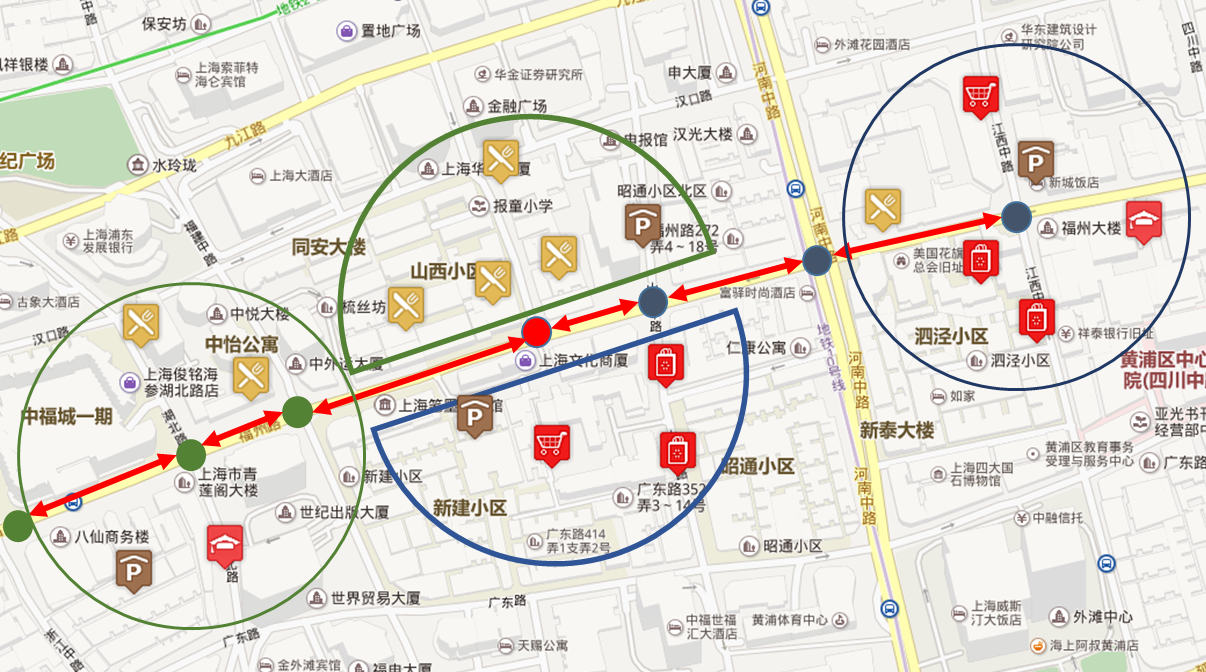
\includegraphics{figures/features/poi.png}}
	\caption{Local Geospatial Features}
	\label{fig:poifeature}
\end{figure}



%While digging on the information we have and brainstorming to achieve a list of features that may become useful, the first set of features that comes into our mind is the information that could best describe the local situation of a given place or point. For example, the road network density in proximity of the node. If the road is along with a lot of crossings with other roads in a relatively small length, it means that there may exists many traffic lights and will inevitably slow the traffic down. The denser network would also imply that many cars will tend to turn right or left other than just going straight. As what we are always trying to do is finding out what may affect the traffic behavior in such a small area, the local features are really important and worth standing out. So we calculated the average distance between the road crossing nodes in both directions from the node. It is trivial by using a formula to calculate the earth distance given two nodes' coordinates.

%Besides the road network density described as the average distance of each road crossing with others, both forward and backward direction, we would also take POIs into great account. If you think the people living in a city's behavior thouroghly, it is actually the points of interests like buildings for work and shopping mall for shopping as well as restaurants for dining that matters the most and affects when and where the people would like to drive to. So the local features on what is besides or near the node on the way is significant. People do go to a specific place or road for some good reasons! From the Baidu Maps points of interest data which we have crawled before, we have manually re-categorized the Baidu's POI types into our own, a total of 37 types. We did investigate the typing hierarchy that Baidu provides and since it is a 2 level tree format, we merged some of the types and also deleted some of the less important ones regarding the behavior of people who drove cars. Then we select all the second level types as ours.

%The features we designed for POIs are in combination of the nearby road crossings related to the previously discussed average distance. In this set of features, we proposed that the POI density of both the current node and the forward and backward nodes located in the next or last road crossing shall have a role. We counted the number of each type of the points of interest around 200 meters away within the node. Such density counting with the same radius parameter is also done for the next 1, 2 and 3 road crossing nodes in both forward and backward directions, as well as the next crossing nodes in the road network both left and right to the direction of the current node's segment. So in total there is 37 types of points of interest for each node, and one given node have 3 level forward crossing point, 3 level backward crossing point, 1 left and 1 right direction crossing nodes, there are $ 37*8=296 $ features being related and attached for each node. It takes a vast majority of our extracted feature list, and by such combination of minor features, there is already cause redundancy, but we considered its importance of preserving information in an obvious way crucial and we can afford to calculate.

\subsubsection{Global Geospatial Features}
\label{sec:globalfeatures}
The above stated local features essentially represent local causes for 
traffic congestions, that is, the causes of the traffic situation are nearby.
Another more subtle scenario is that the cause for congestion on a road segment
is not caused by any road or POI features in the vicinity, but rather because
this road is purely popular during certain time of the day because it connects
or is on the way between two functional areas in the city, 
both of which has a large population using
ground transportation. For example, if a major thoroughfare connects a large
residential area and massive industry park with a lot of companies and factories,
then during morning and evening rush hour, this road will have high chance of
being congested. Driven by this intuition, we focus on three coarse-grain categories
of POIs, namely {\em shopping}, {\em workplace} and {\em residential}.
Most of the 37 types of POIs can be re-categorized into one of the three
categories above. Furthermore, we are only interested in POIs with large
possible population as only these major POIs may cause large flow of traffic
in and out of them. 

To estimate the population density of a POI, we resort to the number of user
comments on a POI on review websites such as dianping.com 
(see the numbers circled in \figref{fig:dianpingexample}), as well as
the number of location-based check-ins from social network such as weibo.com

\begin{figure}[th]
	\centering
	\resizebox{0.8\columnwidth}{!}{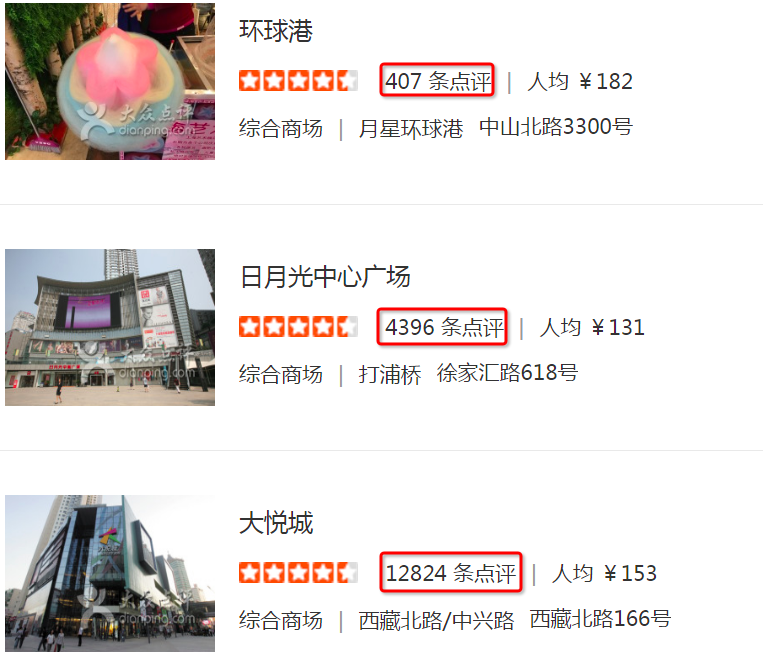
\includegraphics{figures/features/dianping.png}}
	\caption{POI listings of businesses on Dianping.com}
	\label{fig:dianpingexample}
\end{figure}


Then we spatially cluster only those popular POIs from each category
by affinity propagation (AP) algorithm \cite{frey07affinitypropagation}.
The advantage of AP is that we do not need to preset the number 
of clusters. We thus obtain a number of functional areas within 
the city, such as the those shown in \figref{fig:routing}. Here,
blue, purple and red dots represent cluster centers for
residential, shopping and business areas respectively.
Next we compute the fastest routes between any two cluster centers 
over the road network by an A* search algorithm~\cite{4082128}. 
The road network is first remodeled as a 
weighted undirected graph before the routing takes place. 
The weight on each edge is determined by the type of the road 
and its speed limit. An example route 
between two cluster centers is shown as a green line 
in \figref{fig:routing}.

\begin{figure}
	\centering
	\resizebox{\columnwidth}{!}{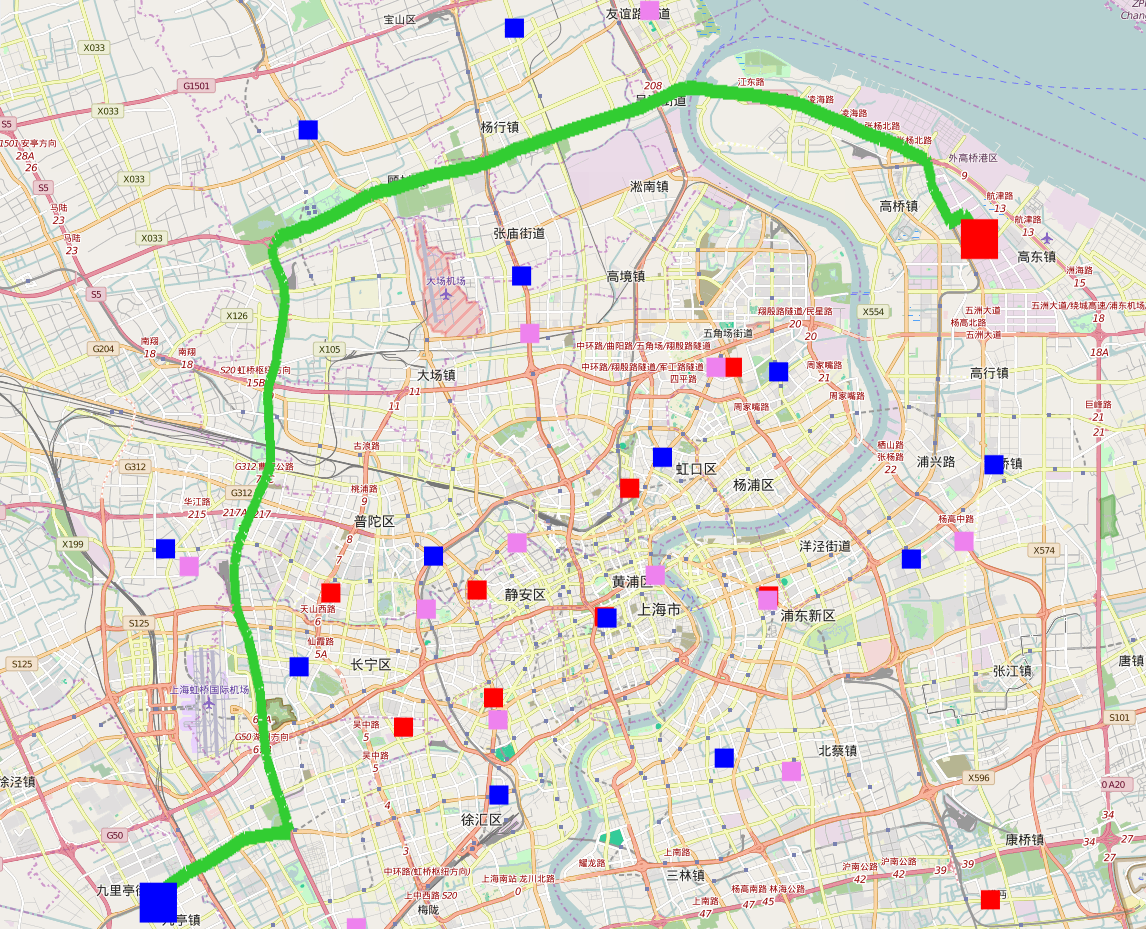
\includegraphics{figures/features/routing.png}}
	\caption{An example graphical output of the optimal routing program from one place to another}
	\label{fig:routing}
\end{figure}

Nine global features are then added to each road node on OSM to represent 
the number of times this node is on the fastest way between any two functional
areas~\footnote{There are $3\times3 = 9$ combinations of travel patterns.}.

%the hot or popular ways, which are the numbers of occurrences for this node to be in the all routes between those 3 clusters of functional areas. To be clear, there are the number of the best routes between residential areas and business site areas that passes just through this particular node, and the number between residential areas and shopping mall areas as well as the number between business sites area and shopping mall areas. In this way, we can have each node having the features that represent the level of popularity of itself as being chosen by people when thinking of driving from on cluster to another.


%As stated in the above section, the local features already play a large part of the roles in the features. However, not all traffic problems and behaviors are only related to the locality of the place where all the cars and traffic goes through. Actually we need to figure out a way to describe and better understand the driver’s motivation and habits. People do not just drive around the city finding the shops or the supermarkets on the sides of the road, they drive every day to work and back home. These commuters are making up a large portion the traffic jam that happens every day on rush hours like in the morning or in the late afternoon on elevated roads, highways, etc. Taking an example in Shanghai for example, many people lives in the suburban areas that is outside the outer ring road of the city. Most of the large companies that is really having large numbers of employees are most possibly located in the urban area inside the middle ring road. A long journey and distance for commuters is a great example showing that local geospatial data are not enough. It does not capture the potential information of where the people would most likely come from and where would they most likely. Temporal data also affecting the problem. In the weekdays, rush hours’ drivers contribute to the most of the traffic jam situations, on the other hand, in the weekend, many people would stay in some shopping mall and going out to the city center to have a nice dinner. The peak traveling hours are varying and changing.

%After proposing that local features are not sufficient, we need to figure out a quantitative set of features that best describe the driver’s preference on roads. Some roads will get really crowded and slow because too many drivers are going to choose the route including the road. For example, every morning and late afternoon, the S4 Hujing Expressway and Humin Elevated Road are both under heavy traffic because there are many people living in the Minhang District of Shanghai, which is a large place for residential areas. The road is also the easiest road to drive that connects the urban area of Xujiahui District, which has all the commercial buildings and shopping malls. Examples like this exists in all aspects of urban life and are quite common. Actually most people on the road lives in the similar place and go to work or eat in the similar places too, and because of the clustering property of human society and urban planning, that gives one of the reasons why roads are crowded. That is we need to identify the “functional areas” in the city that has three types of functionality: shopping, residential and commercial.

%In order to solve this, we need to first find out where people usually live, which is the residential area in the city; where people usually drive to work, which is the business area in the city; and where people usually dine outside and go shopping, which is the commercial area in the city. We need to find out those large clustered points of interest by using clustering algorithms.
%
%\paragraph{Obtaining Data for Clustering}
%Before trying out a variety of the clustering algorithms, we need to collect the raw data first and then apply those algorithms to them. Currently in our database, we have the OpenStreetMap’s geospatial data like road network maps, and the nodes (which we also call them points of interest) crawled, processed and loaded into the database. It seems that we already have solid knowledge base on the sheer number of POIs we have now. However, we lack the popularity of the points of interest information. We wanted to know how many people and how frequently people would go to the specific shopping mall or which building have large amounts of employees that work there. An approach is designed to solve this lack of knowledge problem by cross referencing and collaborate with crawled data of other websites. In our case, we used two external data source, Dianping.com and place.weibo.com, which is both very popular among Chinese people and have a large user base. We primarily used the Dianping.com for the extensive categorical points of interest information of the names, address, rating, price as well as the comments and number of comments of the point. We wrote a Python crawler script to crawl a whole set of data from Dianping.com, mainly consisting 3 types of the functional areas: shopping malls, residential areas and commerce buildings in Shanghai. See Figure~\ref{fig:dianpingexample} for an example page with information of the places. 
%
%After we obtained the places in Shanghai from Dianping.com, we can parse the information of each place obtained. A special program is written to parse the Chinese address shown in the webpage, and extracts only the road name and city name in it. It is actually an address parser using extensive regular expressions to match the address in format that could extract the name of road. The reason for this is to have a better link between the name and address, and better support fuzzy matching while later searching on Weibo Place. Normally there are many shops and restaurants in one shopping mall, and many companies in one business building, so with the help of address parsing, it is much more accurate to find all places associated to that large place. Place.weibo.com is a website for searching location based information that people attached with their status provided by Weibo, a popular social media network in China, that supports searching the place with keywords. Its result is useful for us to determine and quantize the popularity among the people of given place of interest that we obtained earlier in Dianping.com. As shown in Figure~\ref{fig:weiboexample} the information of the search result of a specific place contains the number of posts containing the location, and how many people have come here before and the number of photos users have uploaded.
%\begin{figure}
%	\centering
%	\resizebox{\columnwidth}{!}{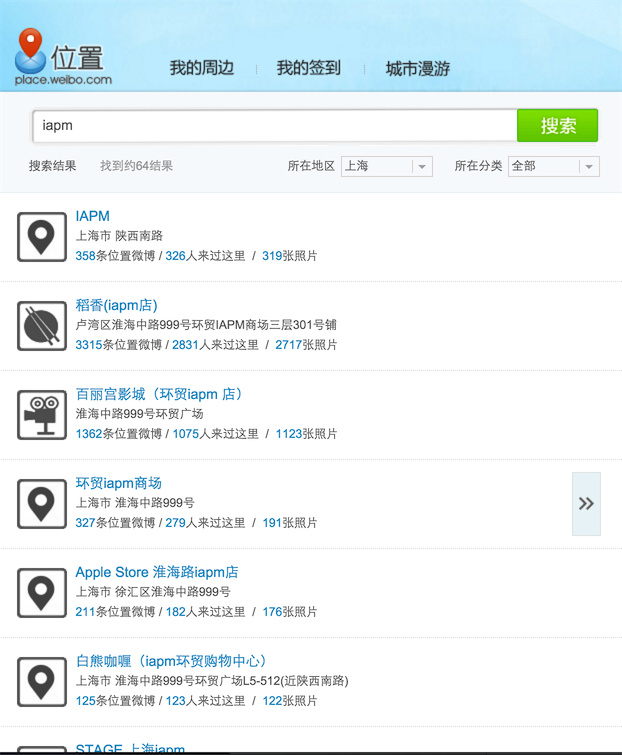
\includegraphics{figures/features/weibo.jpg}}
%	\caption{An example page of the location name search results of Weibo on place.weibo.com}
%	\label{fig:weiboexample}
%\end{figure}
%
%We search for each of the places in Weibo Place by place name that we obtained earlier in Dianping.com and filtered the search result with the road name parsed from the address to ensure that only places with the same address are being counted. The sum of those numbers of posts, photos, check-ins are saved to output file, which will be processed to be our data for clustering later. We sorted by the sum as popularity of the place inside the whole lists of those places, and get a top 1000 most popular list of places of business sites, residential areas and shopping malls. We have made the plots of these data as scattered data in geographical coordinates. See Figure~\ref{fig:businessareas},~\ref{fig:shoppingareas} and~\ref{fig:residencearea} for the distribution and density of each of the 3 functional areas. X-axis dimension is the latitude and Y-axis dimension is the longitude.
%\begin{figure}
%	\centering
%	\resizebox{\columnwidth}{!}{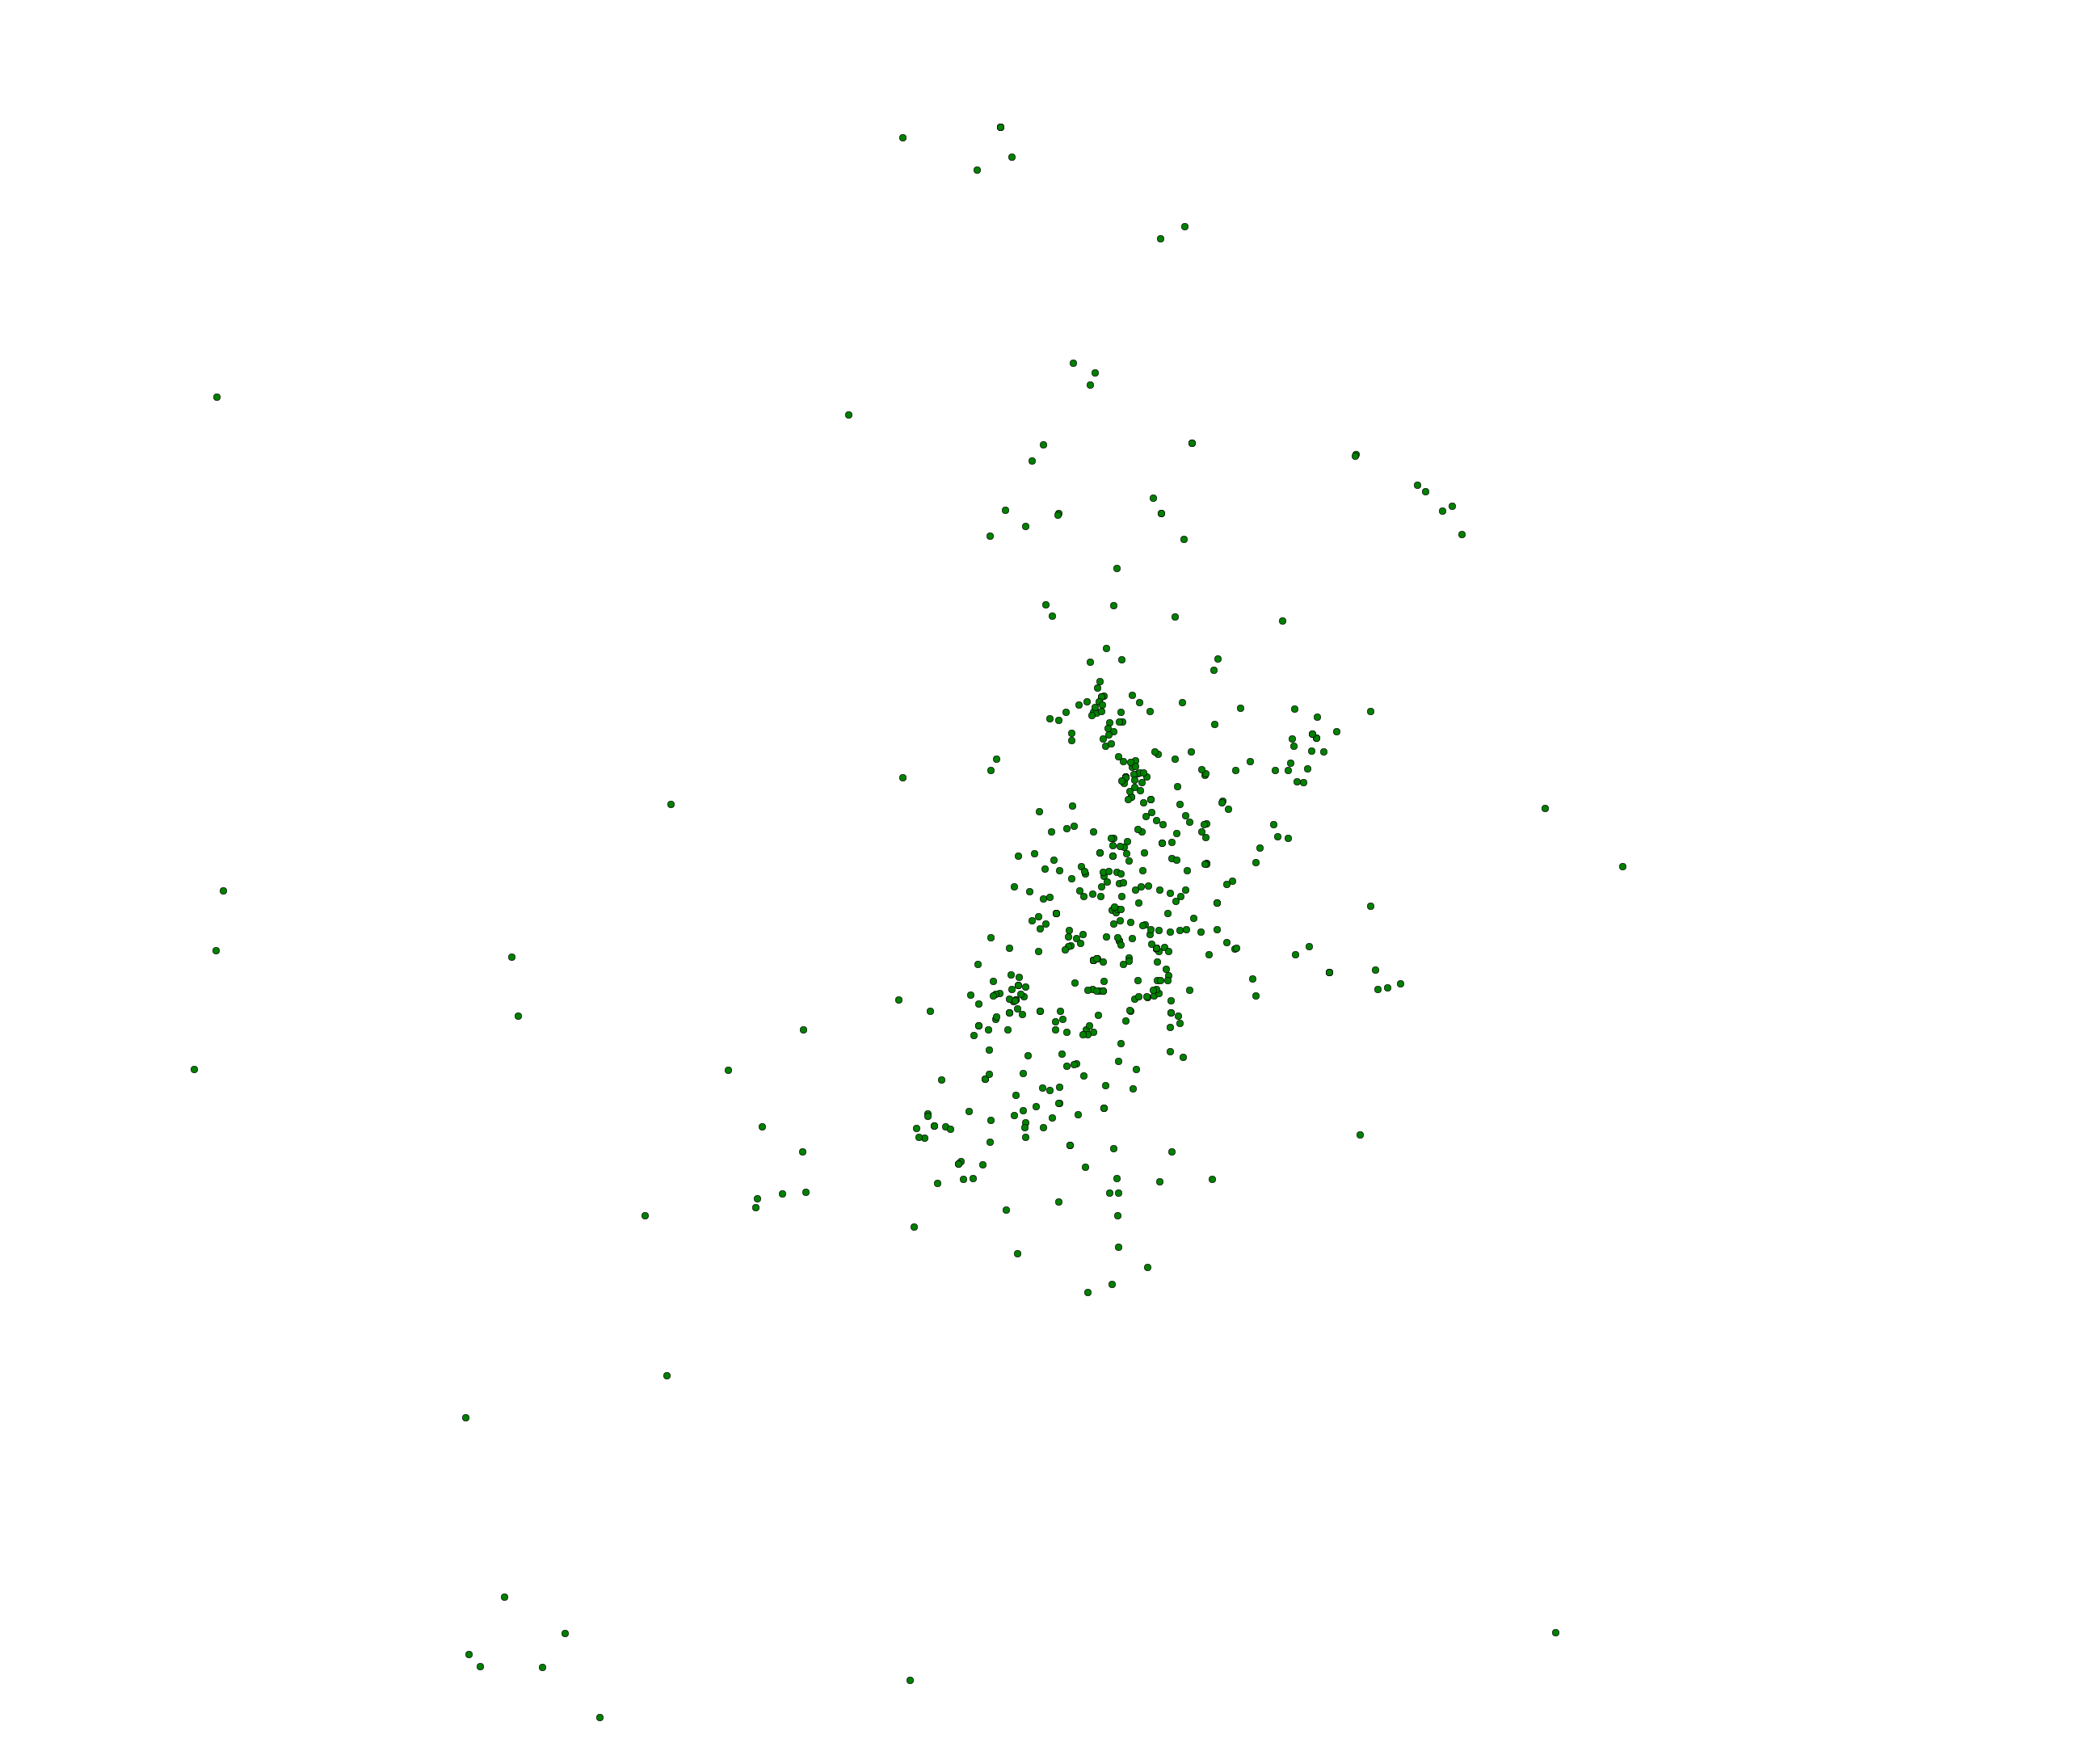
\includegraphics{figures/features/businessSite.png}}
%	\caption{Scattered plot of top business site areas in Shanghai}
%	\label{fig:businessareas}
%\end{figure}
%\begin{figure}
%	\centering
%	\resizebox{\columnwidth}{!}{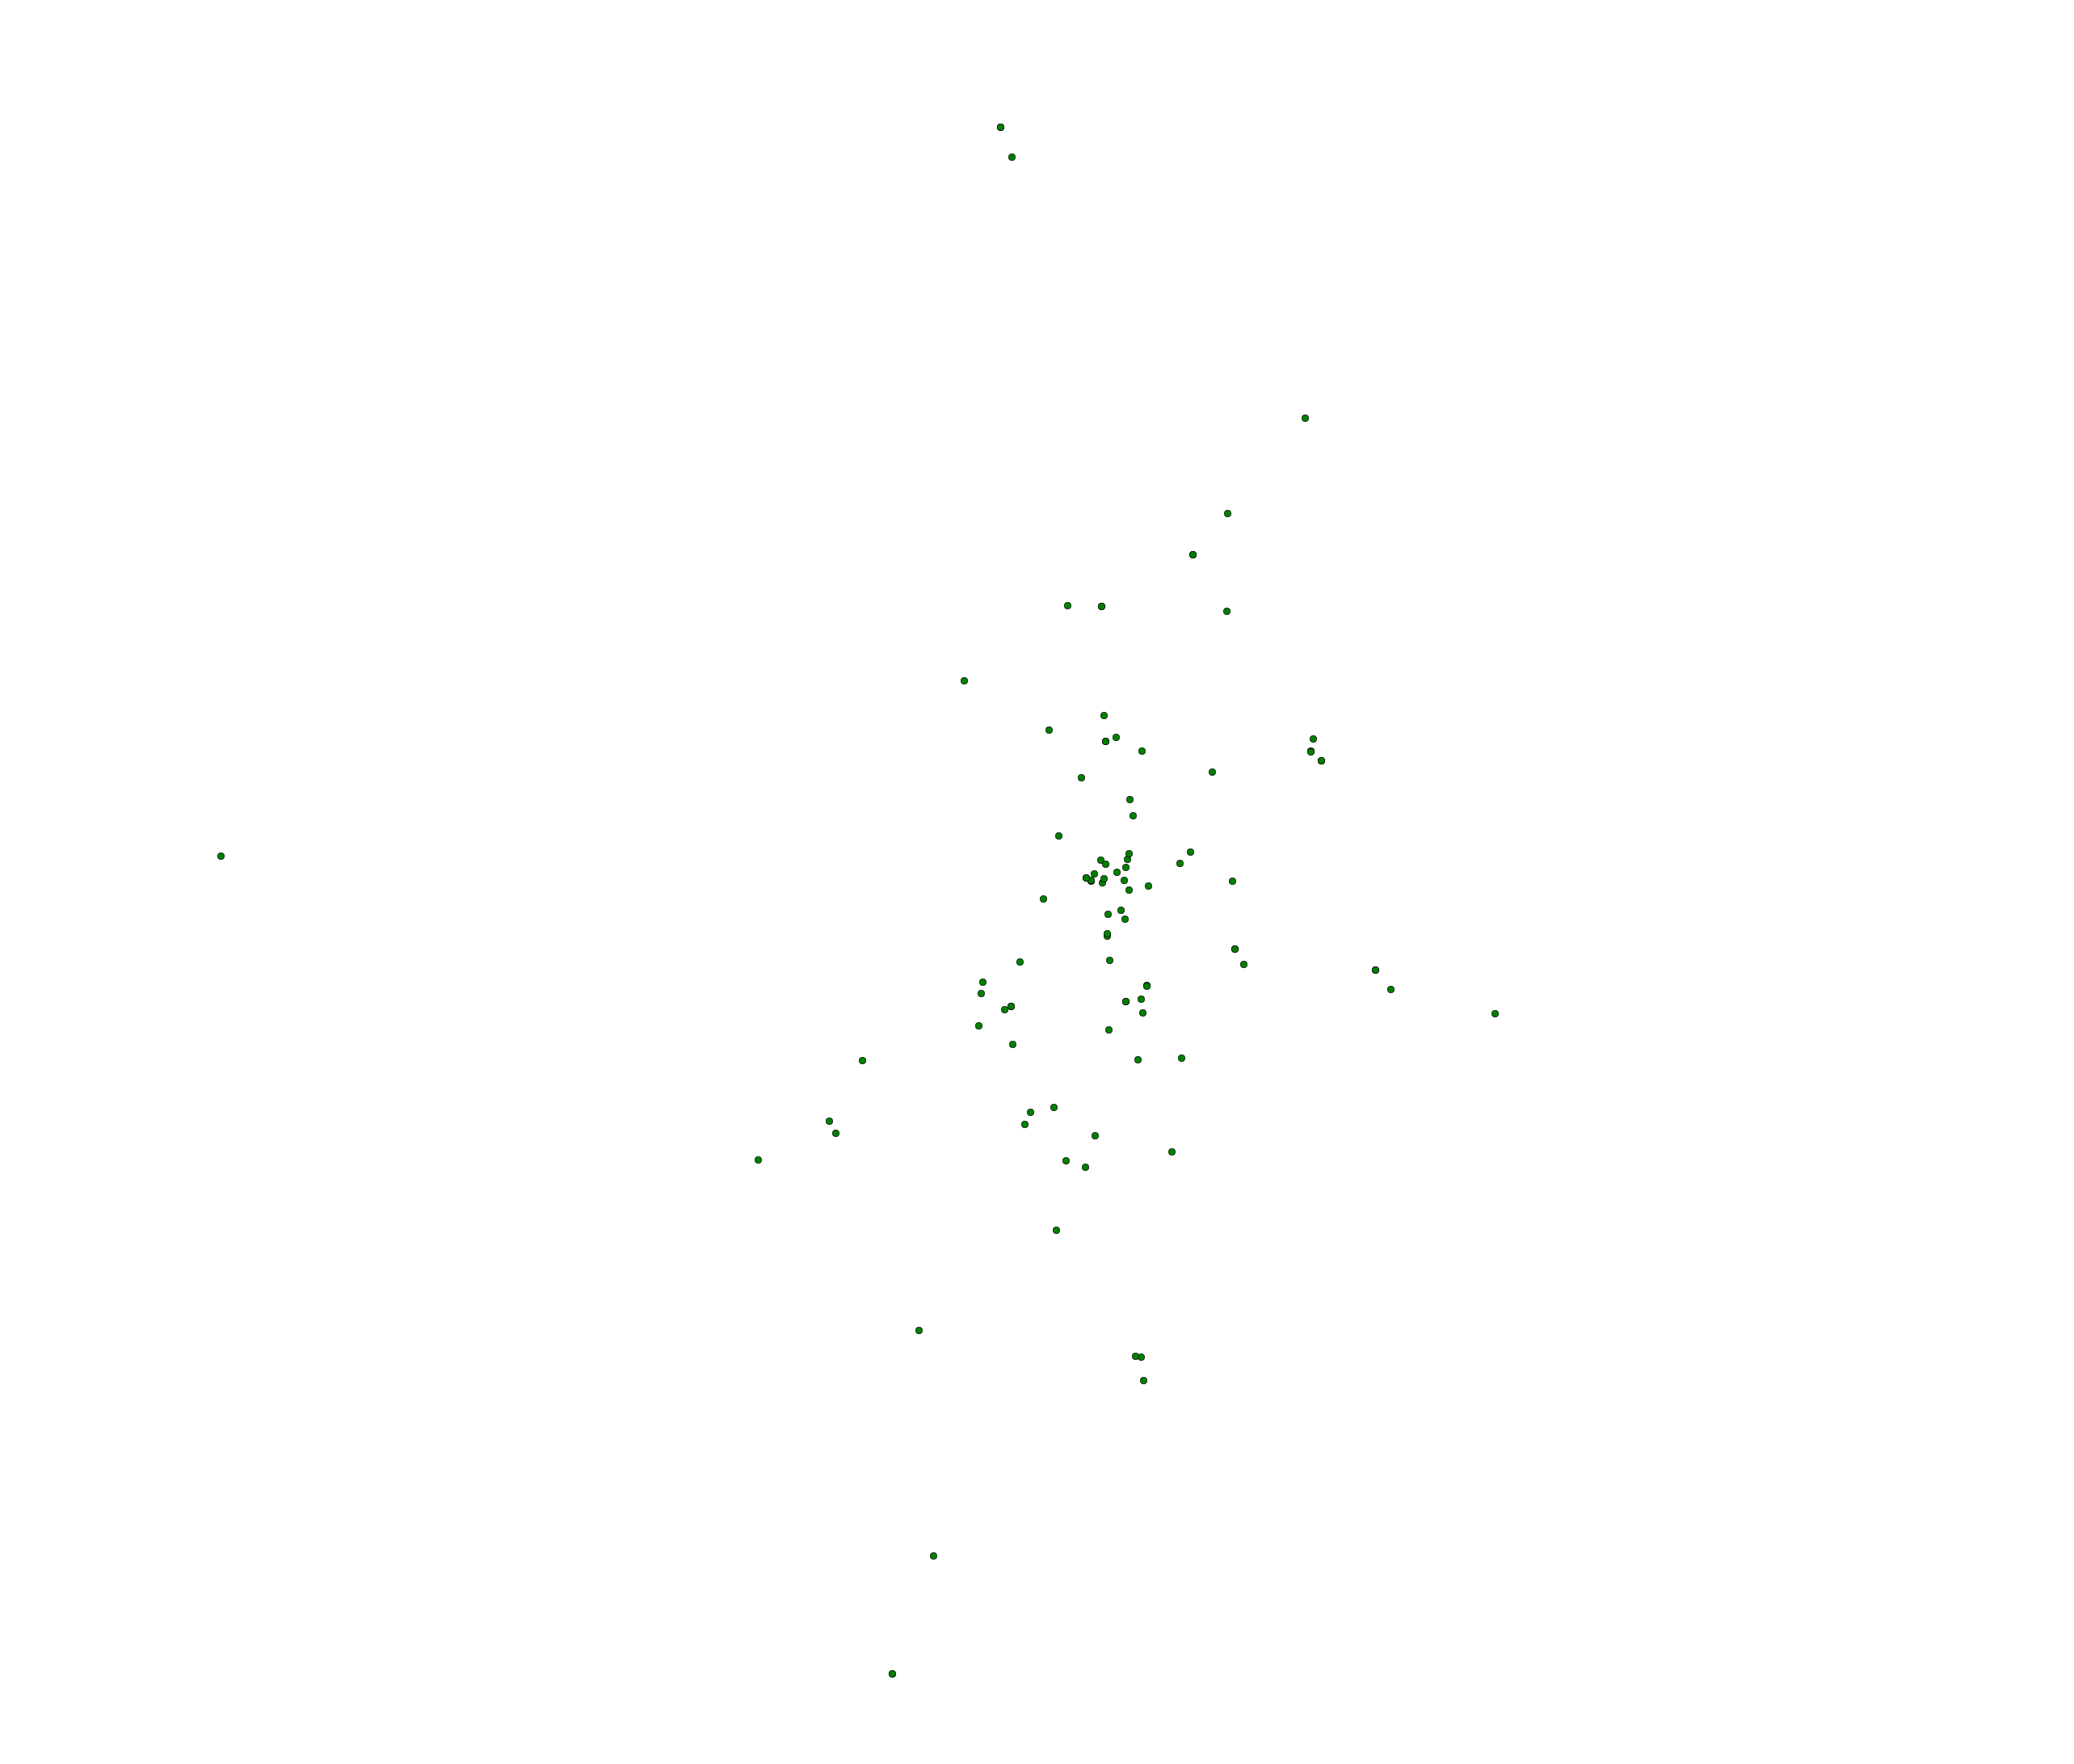
\includegraphics{figures/features/mall.png}}
%	\caption{Scattered plot of top shopping mall areas in Shanghai}
%	\label{fig:shoppingareas}
%\end{figure}
%\begin{figure}
%	\centering
%	\resizebox{\columnwidth}{!}{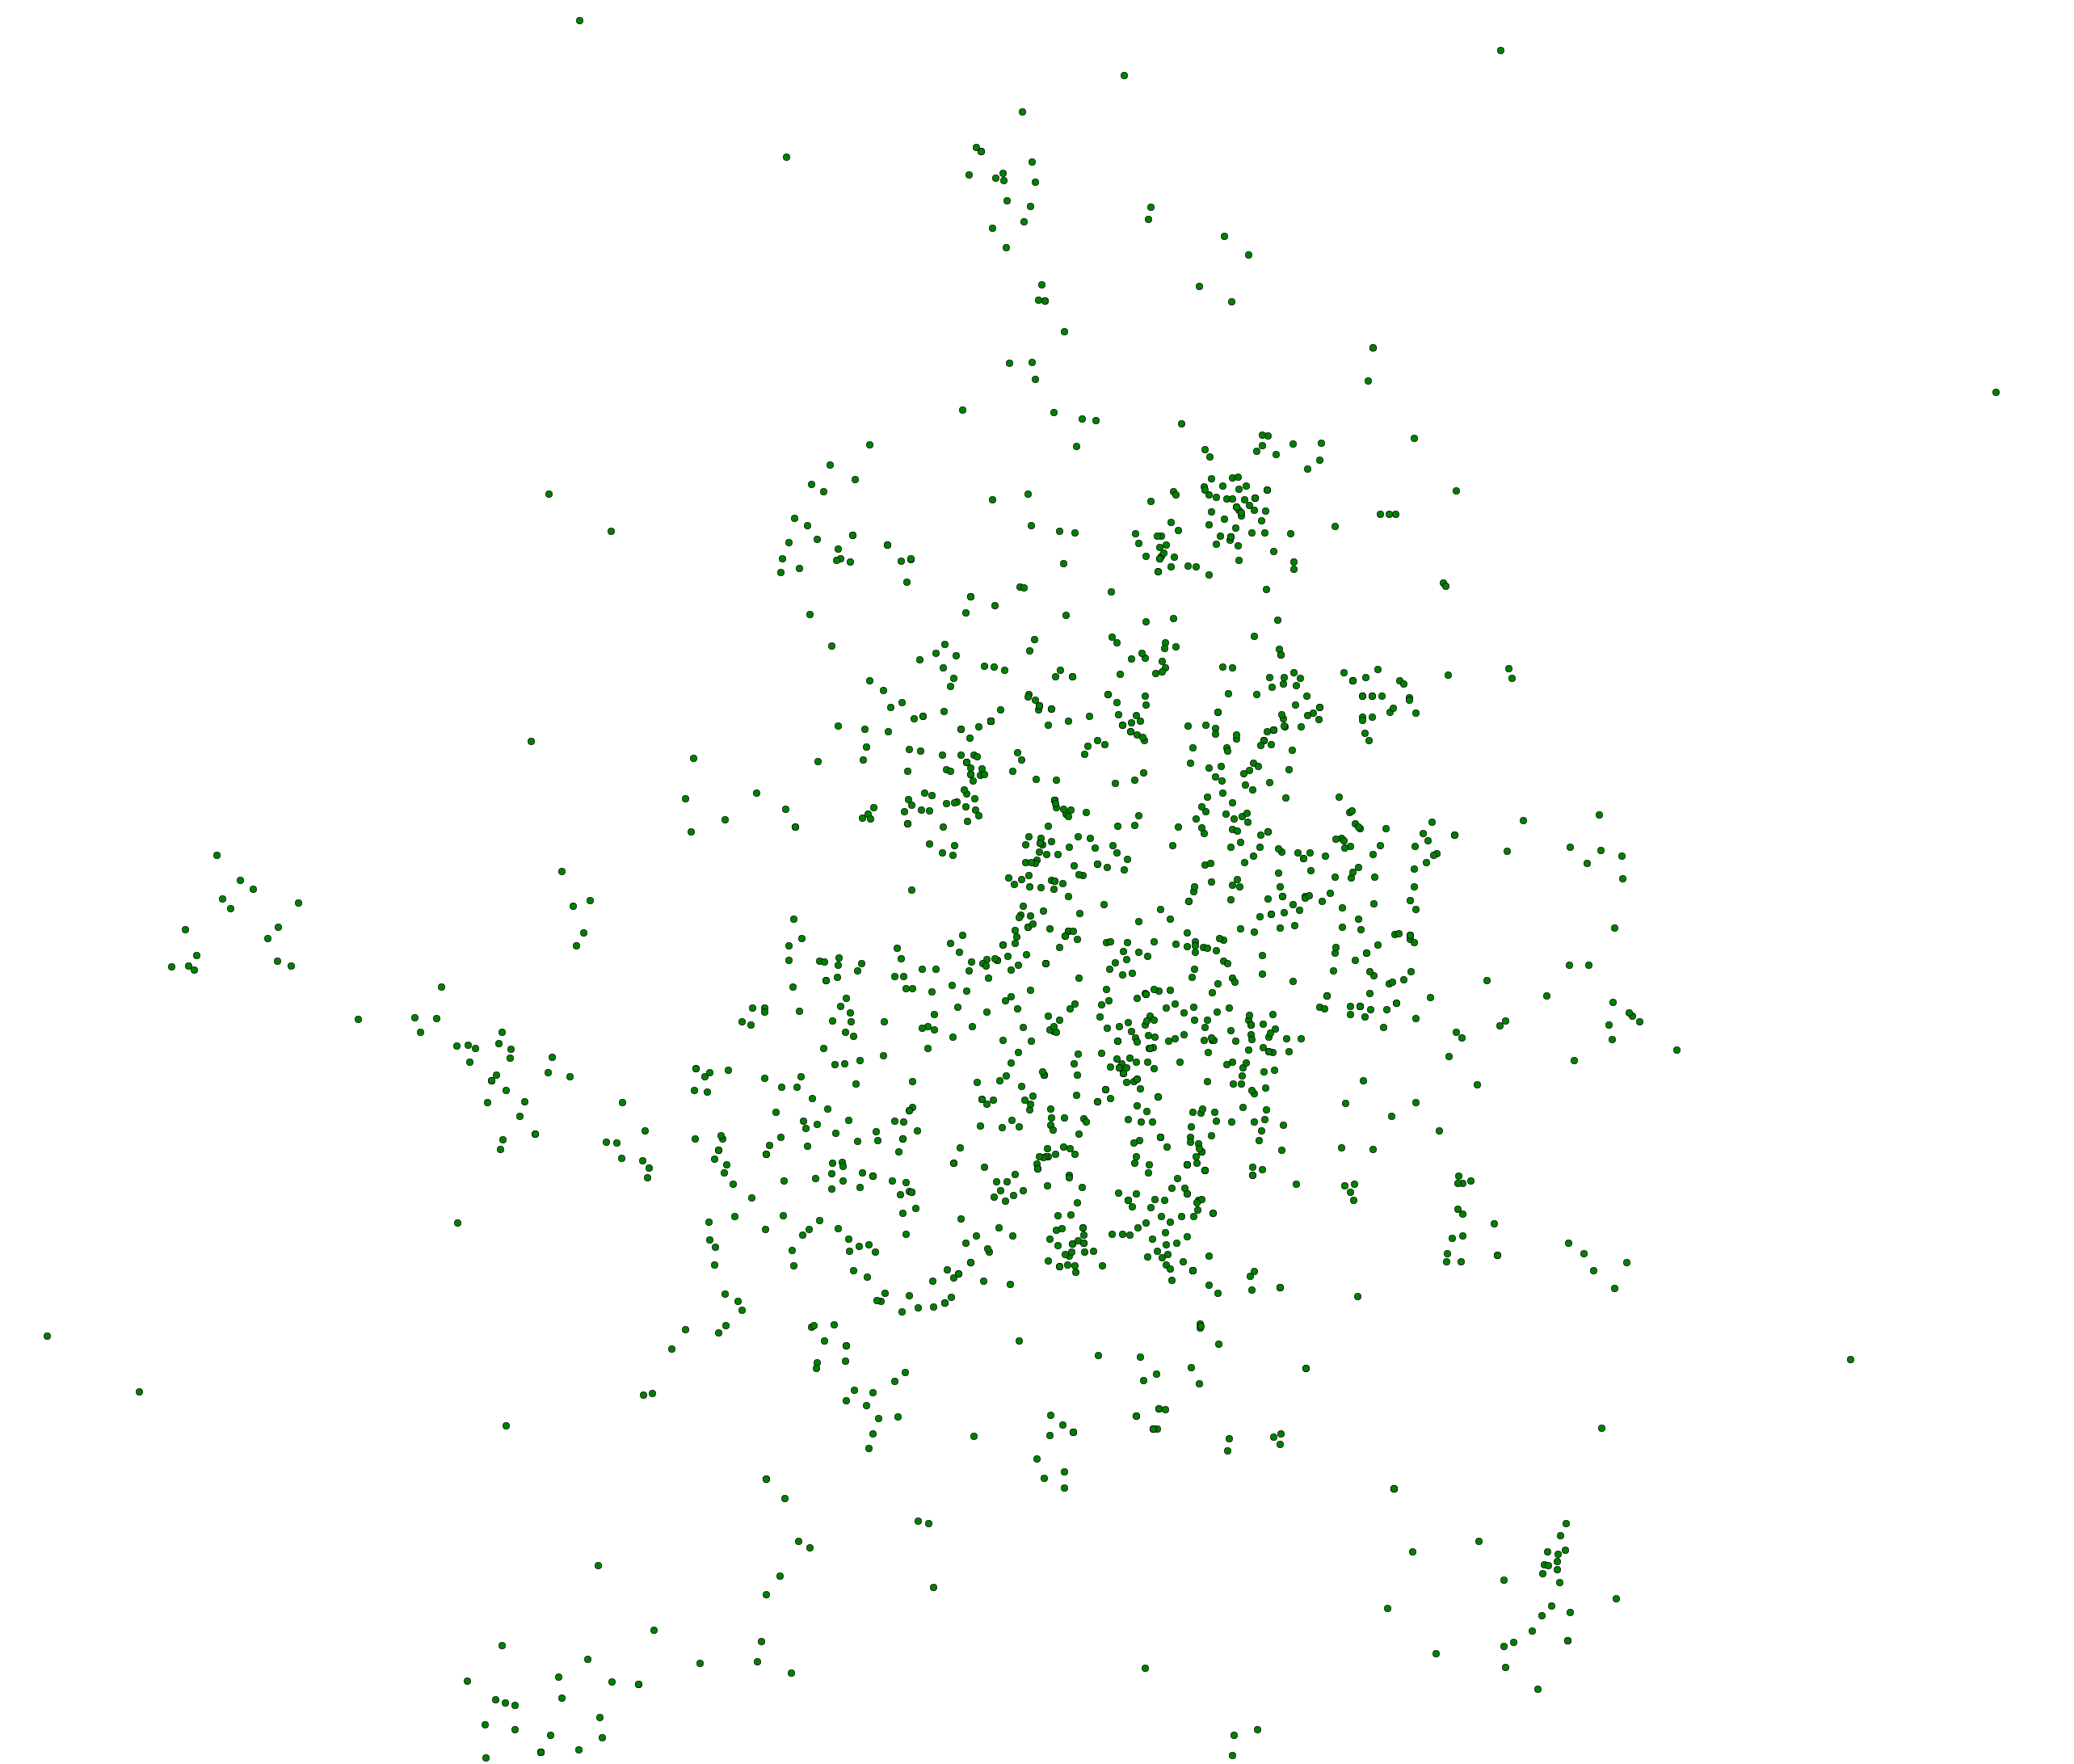
\includegraphics{figures/features/residence.png}}
%	\caption{Scattered plot of top residential areas in Shanghai}
%	\label{fig:residencearea}
%\end{figure}
%
%\paragraph{Clustering the Data Collected}
%Now that we have processed top 1000 most popular lists of three types of places, we can apply the clustering algorithm to find out the clustered functional areas that we wanted. Several of the famous and popular clustering algorithms exist, but the methods of clustering mainly fall into two categories: the first is hierarchical (agglomerative) that initially, each point is in cluster by itself, and then repeatedly combine the two “nearest” into one. The second is point assignment, that is it maintains a set of clusters, and place points into their “nearest” cluster. Many algorithms exist for dealing with such problems, for example the very famous algorithm called the k-means, as well its variant BFR (Bradley-Fayyad-Reina) algorithms for large dataset and some other hierarchical clustering methods, DBSCAN, and Gaussian Mixtures, etc. In this case, however, after studying and experimenting with those algorithms, we selected to use Affinity Propagation algorithm \cite{frey07affinitypropagation}. It's said to be fast, efficient and do not need to specify the number of cluster beforehand, which suits our case well since we want fully automatic clustering without knowing how many those different functional areas there are. It creates clusters by sending messages between pairs of samples until convergence. A dataset is then described using a small number of exemplars, which are identified as those most representative of other samples. The messages sent between pairs represent the suitability for one sample to be the exemplar of the other, which is updated in response to the values from other pairs. This updating happens iteratively until convergence, at which point the final exemplars are chosen, and hence the final clustering is given. Affinity Propagation can be interesting as it chooses the number of clusters based on the data provided. For this purpose, the two important parameters are the preference, which controls how many exemplars are used, and the damping factor.
%The main drawback of Affinity Propagation is its complexity. The algorithm has a time complexity of the order $O(N^2 T)$, where $N$ is the number of samples and $T$ is the number of iterations until convergence. Further, the memory complexity is of the order $O(N^2)$ if a dense similarity matrix is used, but reducible if a sparse similarity matrix is used. This makes Affinity Propagation most appropriate for small to medium sized datasets. 
%
%Algorithm description: The messages sent between points belong to one of two categories. The first is the responsibility $r(i, k)$, which is the accumulated evidence that sample $k$ should be the exemplar for sample $i$. The second is the availability $a(i, k)$ which is the accumulated evidence that sample $ i $ should choose sample $ k $ to be its exemplar, and considers the values for all other samples that $ k $ should be an exemplar. In this way, exemplars are chosen by samples if they are (1) similar enough to many samples and (2) chosen by many samples to be representative of themselves.
%More formally, the responsibility of a sample k to be the exemplar of sample i is given by:
%\begin{align}
%r(i, k) \leftarrow s(i, k) - max [ a(i, \acute{k}) + s(i, \acute{k}) \forall \acute{k} \neq k ]
%\end{align}
%Where $ s(i, k) $ is the similarity between samples i and k. The availability of sample k to be the exemplar of sample i is given by:
%\begin{align}
%a(i, k) \leftarrow min [0, r(k, k) + \sum_{\acute{i}~s.t.~\acute{i} \notin \{i, k\}}{r(\acute{i}, k)}]
%\end{align}
%To begin with, all values for $ r $ and $ a $ are set to zero, and the calculation of each iterates until convergence.
%
%We used the open source machine learning library called scikit-learn \cite{pedregosa2011scikit} which has the affinity propagation algorithm included. So we simply feed the data in with a small Python script and we have some quite amazing clustering result. For example, in the clustering of the data of top business sites obtained earlier, eventually it generates 23 clusters and the Silhouette Coefficient is 0.63. It means that it works relatively good. If the ground truth labels are not known, evaluation must be performed using the model itself. The Silhouette Coefficient is an example of such an evaluation, where a higher Silhouette Coefficient score relates to a model with better defined clusters. The Silhouette Coefficient is defined for each sample and is composed of two scores:
%a: The mean distance between a sample and all other points in the same class.
%b: The mean distance between a sample and all other points in the next nearest cluster.
%The Silhouette Coefficient s for a single sample is then given as:
%\begin{align}
%s = \frac{b - a}{max(a, b)}
%\end{align}
%The Silhouette Coefficient for a set of samples is given as the mean of the Silhouette Coefficient for each sample. The score is bounded between -1 for incorrect clustering and +1 for highly dense clustering. Scores around zero indicate overlapping clusters. The score is higher when clusters are dense and well separated, which relates to a standard concept of a cluster. For clustering result, we can see Figure~\ref{fig:clusteroutput} for the clustered output’s plot of the top business sites found. Those clusters are exactly the functional areas of this particular type that we discussed earlier and at first glance it seems good.
%
%\paragraph{Routing between Functional Areas}
%In the previous chapter, we used the affinity propagation algorithm to cluster the top popular points of interest for each type of the three category. At the time we have three sets of the functional areas of the type business site, residential area and shopping area. We have the knowledge of where they are located at, since the cluster algorithm returns an exemplar for representing the whole nearby area. In order to reflect this information on the road network, we need to find out the connecting routes that people and commuters use for going to work and back home as well as to malls for eating and shopping. Imagine a scenario that a person who lives in Minhang District near Shanghai Jiao Tong University, is working in a company located at Xujiahui. So his living area is actually within the functional area of residence, and Xujiahui is both a business site area and shopping mall area. For his weekdays, he would most probably take the S4 Expressway and into Humin Elevated Road to get to work, so these highways will be under heavy traffic during rush hours, making all the nodes and way segments on it a popular way of choice On Friday night after work for example, he would like to drive to the South Shanxi Road to have dinner in IAPM shopping mall and shop there with his girlfriend, so on such a weekend night, he would take Huaihai Road to move from the business site area to a shopping mall area, and Huaihai Road may become very crowded for this popularity, and so does the nodes on this road. 
%
%In order to find out what ways are popular or not because of the reason that these nodes and segment on this particular way are the connecting components that lies on the road among which is crucial in the most popular routing choice. As many people would use navigation software, finding the recommended routes between those discovered types of functional areas now proves to be important.
%
%When talking about routing algorithms on a road network, we would instantly consider the map information being represented as a directional graph with weight on the edges. The edges would be the road segments connecting nodes. Our new problem of finding the most popular route between two locations now is being translated into the problem of finding the shortest path in a large graph between two vertices. To be more accurate, it should be the cheapest cost path because we do not just want the route that is short in mere distance, we would like to take road type and so on into consideration. So a weighted shortest path problem should best describe this, and the weight is affected by road type, for example the elevated roads or highway that have a better speed and priority should cost less weight than the secondary and ordinary roads with crossings and traffic lights making them more favorable. Also, one-way is also an important deciding factor in routing algorithms because it would simply disable or prohibit such edges being reached in certain direction. In our database there is always a tag with the way elements, showing the road hierarchy and one-way flag.
%
%We consider a directed graph $ G = (V,E) $ with n nodes and $ m = Θ(n) $ edges. An edge $ (u,v) $ has the non-negative edge weight $ w(u,v) $. A shortest-path query between a source node $ s $ and a target node $ t $ asks for the minimal weight $ d(s, t) $ of any path from $ s $ to $ t $. In static routing, the edge weights do not change so that it makes sense to perform some pre-computations, store their results, and use this information to accelerate the queries. Obviously, there is trade-off between query time, pre-processing time, and space for pre-processed information. In particular, for large road networks it would be prohibitive to pre-compute and store shortest paths between all pairs of nodes.
%
%Dijkstra’s Algorithm \cite{dijkstra1959note} is the classical algorithm for route planning—maintains an array of tentative distances $ D[u] ≥ d(s, u) $ for each node. The algorithm visits (or settles) the nodes of the road network in the order of their distance to the source node and maintains the invariant that $ D[u] = d(s, u) $ for visited nodes. We call the rank of node $ u $ in this order its Dijkstra rank $ rks(u) $. When a node u is visited, its outgoing edges $ (u,v) $ are relaxed, i.e., $ D[v] $ is set to $ min(D[v], d(s, u) + w(u,v)) $. Dijkstra’s algorithm terminates when the target node is visited. The size of the search space is $ O(n) $ and $ n/2 (nodes) $ on the average. We will assess the quality of route planning algorithms by looking at their speedup compared to Dijkstra’s algorithm, i.e., how many times faster they can compute shortest-path distances.
%
%The algorithm that we use in our routing purpose is A* Search algorithm \cite{4082128}, also known as Geometric Goal Directed Search. The intuition behind goal directed search is that shortest paths ‘should’ lead in the general direction of the target. A* search achieves this by modifying the weight of edge $ (u,v) $ to $ w(u,v)−π(u) + π(v) $ where $ π(v) $ is a lower bound on $ d(v,t) $. Note that this manipulation shortens edges that lead towards the target. Since the added and subtracted vertex potentials$  π(v) $ cancel along any path, this modification of edge weights preserves the shortest paths. Moreover, as long as all edge weights remain non-negative, Dijkstra’s algorithm can still be used. The classical way to use A* for route planning in road maps estimates $ d(v,t) $ based on the Euclidean distance between $ v $ and $ t $ and the average speed of the fastest road anywhere in the network. Since this is a very conservative estimation, the speedup for finding the quickest routes is rather small. Lastly there is heuristic that evolved during recent years. In the last decades, commercial navigation systems were developed which had to handle ever more detailed descriptions of road networks on rather low-powered processors. Vendors resolved to heuristics still used today that do not give any performance guarantees: use A∗ search with estimates on $ d(u,t) $ rather than lower bounds; do not look at ‘unimportant’ streets, unless you are close to the source or target. The latter heuristic needs careful hand tuning of road classifications to produce reasonable results but yields considerable speedups.
%
%In the engineering process, we implemented A* algorithm to read the OpenStreetMap data format, along with two coordinates representing the starting point and ending point of the routing. We used the tags about the road that the ways in the database have to create a customized weight for different type of roads. We are routing each location in the clustered functional areas to those other locations in another type of functional areas. So we have 3 groups of routing being done: the routes between locations in residential areas and business sites areas, the routes between locations in residential areas and shopping mall areas, and the routes between locations in business sites areas and shopping mall areas. An example routing after running our program is plotted in Figure~\ref{fig:routing}, note that the map plots all valid roads of the bounded area in Shanghai, and the red polylines which take a large majority is the roads that has not been searched. Those in blue are the roads that the A* algorithms runs through and calculated. The green one is the final optimal route found. We have all the node ID and way ID information so that we can identify easily.
%

\subsubsection{Non-Geospatial Implicit Features}

The following features are not properties of the map, but may have implicit impact
on the population density of an area, the drivers behaviros, or the travel patterns.
We proposed 8 features in this category: 
\begin{itemize}
\item the time of the day (in hours); 
\item weekday or weekend; 
\item the 1-, 2- and 3-bedroom apartment rental price in the area; 
\item the temperature in the day and night; and 
\item the weather condition of the time (i.e., sunny, cloudy, shower or rainy, etc.). 
\end{itemize}
%It is quite straightforward for us to come up with these features, they can have linkage with the traffic situation. For example, the rental price of the nearby apartment reflects the popularity, population and land price of the area, which shall further imply the degree of importance and centrality in urban area. There are really some expensive residential areas in Shanghai like near the center of the city in Huangpu District, where the population is really high. The population density is a crucial matter that affects traffic. If the rental price is high, it means that there lives a high density of people, and as a result, the traffic vehicles that travels from and to this place will be massive, resulting in heavy traffic. So we think it is a significant feature that represents the population density of the area, the distribution over area data of which is hard for us to obtain. 

%Other features like the time of the day and the difference between weekdays and weekends are also self-explanatory: people have different goals and motivation of where they would like to drive to on weekdays and weekends, which will affect road network loads and as a result causing traffic problems. In rush hour of weekdays, the roads' connection where most people live and where the workplaces being located at are getting large flow of traffic. On weekends however, roads connecting the residential functional areas and shopping mall areas during the dinning time and the closing hour of the shopping mall will also become under heavy congestion. Other features like weather and temperature of the area are also straightforward and guaranteed to have positive effects on prediction results. When the weather is rainy and bad, by all our consensus, people tend to drive more than walking and taking public transit because of the bad weather makes people reluctant to spend time outside and rather to stay inside the cars. Also the speed of vehicle under bad weathers are lower than normal, contributing to the congestion. Extremely low and high temperatures will also cause the people drive more often because there is air conditioning inside and without the hassle and of walking outside.

%In summary, here we list all the features we discussed in this
%section. 
%%
%%
%%
%\begin{itemize}\itemsep0pt
%	\item local geo-spatial
%	\begin{itemize}\itemsep0pt			
%		\item POI
%		\item road density
%		\item road type
%		\item haveshop 
%	\end{itemize}
%	
%	\item global geo-spatial
%	\begin{itemize}\itemsep0pt			
%		\item routing
%	\end{itemize}
%	\item non-geo-spatial
%	\begin{itemize}\itemsep0pt			
%		\item price
%		\item temperature
%		\item weather
%		\item hour
%		\item isweekend
%		\item isRushHour
%	\end{itemize}
%\end{itemize}

%with a total number of 311. Note that the weather condition feature is represented as a binary representation of 1-in-N representation, see Section~\ref{sec:modelextractfeature} for details. Some of those features are input by user as prior knowledge during the prediction step. Though with different source and magnitude, either explicitly or implicitly representing the causing factors, they, being put together, comprise a large set of knowledge engineered by either we researchers as well as the computer algorithms, and that is one of the most important step and effort in application machine learning in real world scenarios.

% DO WE NEED TO ADD FEATURE LIST HERE?


%!TEX root = paper.tex
\section{InferSpark Overview}
\label{sec:framework}

\begin{figure*}[th]
	\centering
	\includegraphics[width=1.6\columnwidth]{figs/workflow2.eps}
	\caption{InferSpark Architecture}
	\label{fig:workflow}
\end{figure*}

%\KZ{My general feeling is that the running example is not made full use of.
%The discussion should be tightly coupled to the running example. E.g., when
%we talk about schedule, just present the schedule for the two coins.
%Some of the stuff here should go into implementation section.}

The overall architecture of InferSpark is shown in \figref{fig:workflow}. 
An InferSpark program is a mix of Bayesian network model definition and
normal user code. The Bayesian network construction module separates the
model part out, and transforms it into a Bayesian network template. This
template is then instantiated with parameters and meta data from the input
data at runtime by the code generation module, which produces the VMP inference
code and message passing graph. These are then executed on the GraphX 
distributed engine to produce the final posterior distribution.
%InferSpark analyzes the Bayesian network defined by a special 
%scala-like program and
%automatically transforms the model definition into the GraphX implementation
%of VMP algorithm. After two stages of compilation, the runtime system 
%launches the VMP implementation and returns the inference results 
%through the query API.  
Next, we describe the three key modules in more details with 
the example of the two-coin model (\figref{fig:two_coin_bn}).

\subsection{Running Example}

\begin{figure}[h]
\begin{lstlisting}
@Model class TwoCoins(alpha: Double, beta: Double) {
	val pi = Beta(alpha)
	val phi = (0L until 2L).map(_ => Beta(beta))
	val z = ?.map(_ => Categorical(pi))
	val x = z.map(z => Categorical(phi(z)))
}
object Main {
	def main() {
		val xdata: RDD[Long] = /* load (observed) data */
		val m = new TwoCoins(1.0, 1.0)
		m.x.observe(xdata)
		m.infer(steps=20)
		val postPhi: VertexRDD[BetaResult] = m.phi.getResult()
		/* postprocess */
		...
	}
}
\end{lstlisting}
\caption{Definition of two-coin model in InferSpark}
\label{fig:two_coins_modeldef}
\end{figure}

%Apart from ordinary scala code, the input program of InferSpark contains the
%statistical model definitions. The syntax of the model definition extends
%from the scala syntax.  
\figref{fig:two_coins_modeldef} shows the definition of the two-coin model
in InferSpark. The definition starts with ``{\sf @Model}'' annotation. 
The rest is similar to a class definition in
scala. The model parameters (``{\sf alpha}'' and ``{\sf beta}'') are constants to the
model. In the model body, only a sequence of value definitions are allowed,
each defining a random variable instead of a normal deterministic variable. 
The use of ``{\sf val}'' instead of ``{\sf var}'' in the syntax 
implies the conditional dependencies between random variables are fixed 
once defined. For example, line
2 defines the random variable $\pi$ having a symmetric Beta prior
$\mathrm{Beta}(\alpha, \alpha)$.

InferSpark model uses ``Range'' class in Scala to represent plates. Line 3
defines a plate of size 2 with the probabilities of seeing head in the 
two coins. The ``?'' is a special type of ``Range'' representing 
a plate of unknown size at the time of model definition. 
In this case, the exact size of the plate will be provided or inferred
from observed variables at run time.  When a random variable is
defined by mapping from a plate of other random variables, 
the new random variable is in the same plate as the others.  
For example, line 5 defines the outcomes $x$ as the mapping from $z$ 
to Categorical mixtures, therefore $x$ will be in the same plate as
$z$. Since the size of the plate surrounding $x$ and $z$ is unknown, we need
to specify the size at run time.  We can either explicitly set the length of
the ``?'' or let InferSpark set that based on the number of observed outcomes
$x$ (line 11).

At the first glance, ``?'' seems redundant since it can be replaced by a
model parameter $N$ denoting the size of the plate.  However, ``?'' becomes
more useful when there are nested plates. In the two-coin model, suppose
after we choose one coin, we toss it multiple times. 
\figref{fig:two_coins_nestedplates} shows this scenario.
Then the outcomes $x$ are in two nested plates where the inner plate is
repeated $M$ times, and each instance may have
a different size $N_i$. Using the ``?'' syntax
for the inner plate, we simply change line 5 to
{\small\begin{verbatim}
	val x = z.map(z => ?.map(_ => Categorical(phi(z))))	
\end{verbatim}
}

\begin{figure}[th]
	\centering
	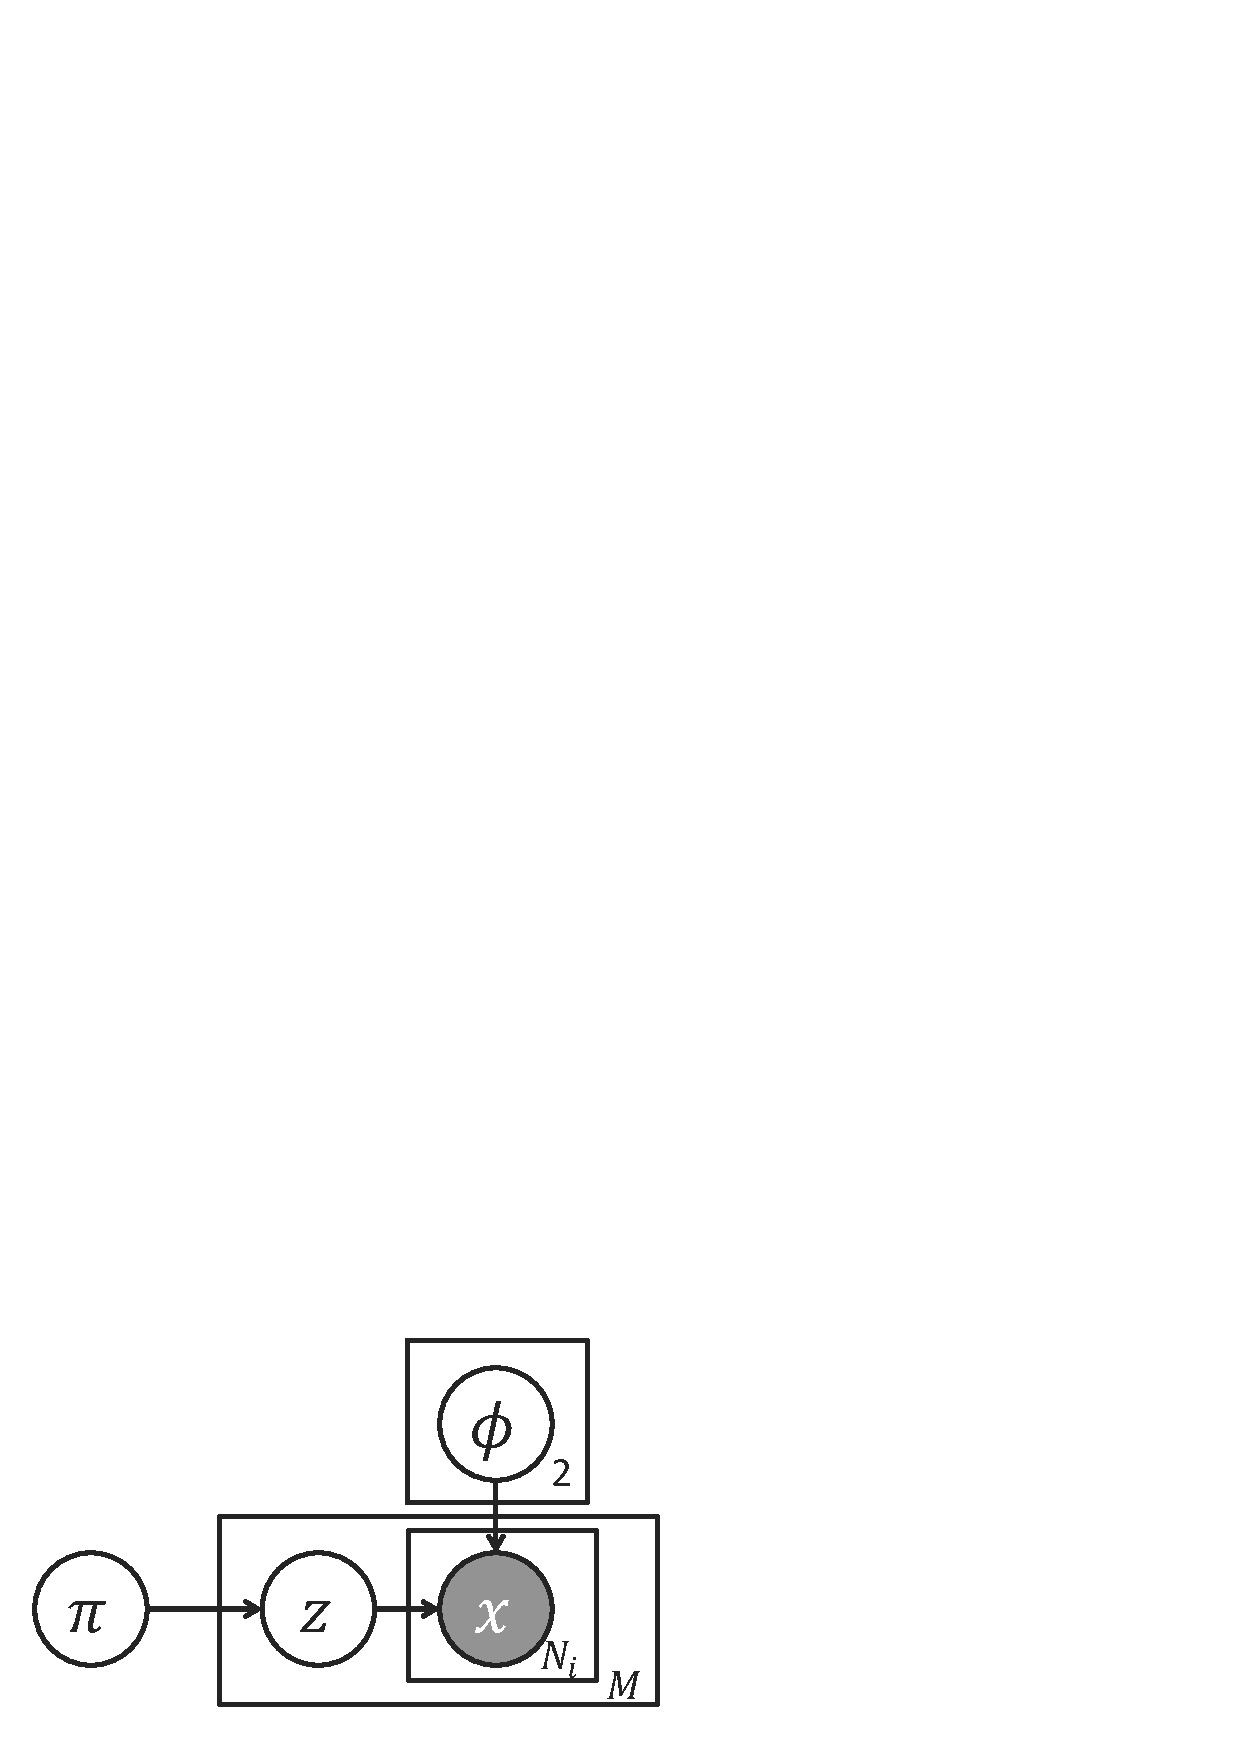
\includegraphics[width=0.25\textwidth]{figs/two_coins_nestedplates}
	\caption{Two-coin Model with Nested Plates}
	\label{fig:two_coins_nestedplates}
\end{figure}

\subsection{Bayesian Network Construction}

\begin{figure}[h]
\centering
\includegraphics[scale=0.4]{figs/two_coins_bn1.eps}
\caption{Bayesian Network Template Constructed from the Two-coin Model}
\label{fig:two_coins_bn1}
\end{figure}

An input InferSpark program is first parsed and separated into two parts: 
the model definition (``{\sf @Model} class TwoCoins'' in 
\figref{fig:two_coins_modeldef}) and
the ordinary scala program (``{\sf object Main}'' in
\figref{fig:two_coins_modeldef}). The model definition is analyzed and
transformed into valid scala classes that define a Bayesian
network constructed from the model definition 
(e.g., \figref{fig:two_coins_bn1}) and the inference/query API.
Note the Bayesian network
constructed at this stage is only a template (different than 
\figref{fig:two_coin_bn}) because some of the information is not available 
until run time (e.g., the outcomes $x$, the number of coin flippings 
and the model parameters $\alpha$ and $\beta$). 
%A snippet of generated two-coin code (with simplified variable names)
%is shown in \figref{fig:two_coins_stage1code}.
%
%\begin{figure}[h]
%\centering
%\begin{lstlisting}
%class TwoCoins(alpha: Double, beta: Double) extends ModelBase {
%	val synval$internal$parent: Array[Int] = /**/
%	var Categorical$13$isObserved: Boolean = _
%	class Categorical$13$Inferface extends RandomVariable {
%		def observe(obs: RDD[Long]) = /* ... */
%		def getResult(): RDD[CategoricalResult] = /* ... */
%	}
%	val x = new Categorical$13$Interface()
%	/* ... */
%}
%\end{lstlisting}
%\caption{Bayesian Network Code}
%\label{fig:two_coins_stage1code}
%\end{figure}
%
%The Bayesian network source code is then compiled with the
%ordinary scala program into bytecode. This bytecode will generate the
%inference code of the VMP algorithm for the model on GraphX in
%the next 4 steps.
%
%The InferSpark model definition is a scala definition with ``@Model''
%annotation. The scala parser first separates the model definition from other
%part of the program (i.e. user program). A Bayesian network is then constructed
%according to dependencies between the random variables in the model definition.
%\figref{fig:lda_bn1} is the Bayesian network constructed from the LDA model
%definition. Some information only available at runtime are missing from the
%Bayesian network, e.g. the number of topics $K$, the observed words $w$, etc.
%At this step, the analyzer also verifies that the model is in the
%exponentail-conjugate family and rejects unsupported model definitions. After
%the construction, the Bayesian network is stored in the compiled program for
%later steps to process.

%\begin{figure}[!h] 
%	\centering 
%	\includegraphics[scale=0.3]{figs/lda_bn1.eps}
%	\caption{Bayesian Network Constructed From the Model Definition}
%	\label{fig:lda_bn1}
%\end{figure}

\subsection{Metadata Collection}

Metadata such as the observed values and the plate sizes missing from the
Bayesian networks are collected at runtime. In the two-coin
model, an instance of the model is created via the constructor invocation (e.g.
``{\sf val m = new TwoCoin(1.0, 1.0)}'' on line 10 of \figref{fig:two_coins_modeldef}). The constructor call provides
the missing constants in the prior distributions of $\pi$ and $\phi$. 
For each random variable defined in the model definition, 
there is an interface field with the
same name in the constructed object. Observed values are provided to InferSpark
by calling the ``{\sf observe}'' (line 11 of \figref{fig:two_coins_modeldef}) 
API on the field. 
There, the user provides an RDD of observed outcomes ``{\sf xdata}'' to InferSpark by calling
``{\sf m.x.observe(xdata)}''. The  {\sf observe} API also triggers 
the calculation of unknown plate sizes. 
In this case, the size of plate surrounding $z$ and $x$ is
automatically calculated by counting the number of elements in the RDD.

%When the user provide the observed random variables such as the words in the
%LDA model, the number of documents and the number of words in each document
%can be inferred from the data. This is different from most libraries in that
%they require the user to explicitly set the numbers or to transform the data
%into a library-specific format. InferSpark also tries to verify that the user
%have provided consistent data. For example, InferSpark will report an error,
%if the user provides data to both the topics $z$ and the words $w$ but they
%have differnt sizes.

\subsection{Code Generation}

\begin{figure}
\centering
	\includegraphics[width=0.35\textwidth]{figs/two_coins_msg.eps}
	\caption{Bayesian Network with Messages for Two-coin Model}
	\label{fig:two_coins_msg}
\end{figure}

When the user calls ``{\sf infer}'' API (line 12 of \figref{fig:two_coins_modeldef}) 
on the model instance, InferSpark
checks whether all the missing metadata are collected. If so, it proceeds to
annotate the Bayesian network with messages used in VMP, resulting in
\figref{fig:two_coins_msg}. The expressions that calculate the messages 
(e.g., $E_{Q_\pi}[\ln \pi]$) depend on not only
the structure of the Bayesian network and whether the vertices are observed or
not, but also practical consideration of efficiency and constraints on
GraphX.  

%The inference algorithm we use is the variational message passing algorithm.
%This step annotates the messages and vertex updates of the algorithm to the
%Bayesian network from previous step and we call the resuling graph as message
%passing graph.
%
%The VMP algorithm is expressed as sending messages of functions of sufficient
%statistics of random variables and updating the sufficient statistics by
%aggregating the messages. The messages are sent in both direction of the edges
%in the Bayesian network. The vertices are updated by aggregating incoming
%messages. For the Dirichlet random variables, the update is simply adding
%together all the messages. The unobserved Categorical random variable $z$ is
%updated by normalizing the sum of the messages. The observed Categorical
%mixtures $w$ have nothing to update but have to compute the new messages to $z$
%and $\phi$ according to the incoming messages.

%\begin{figure}[h]
%	\centering	
%	\includegraphics[scale=0.3]{figs/lda_mpg.eps}
%	\caption{Message Passing Graph of LDA}
%	\label{fig:lda_mpg}
%\end{figure}


%The messages in the VMP algorithm are sent in both directions. The messages
%along the edge only depend on the sender but the messages in the reverse
%direction may also depend on other parents' message.  For example, the message
%along the edge from $z$ to $w$ only depends on the sufficient statistics of
%the Categorical variable $z$, but the reverse one will depend on the
%topic-word distributions' messages. The original VMP algorithm assumes that
%only one vertex may be updated in each step and the messages that the vertex
%depends on are always up-to-date.  However, this poses two challenges when
%implementing it as a distributed message passing algorithm. First, we have to
%relax the assumption of one vertex in each step to increase parallelism
%without violating the correctness of the algorithm. In the LDA example,
%Updating all the random variables at the same time does not guarantee to
%optimize the ELBO but we can update all the topics at the same time because it
%is equivalent to sequentially update each of the topics. Secondly, vertecies
%that have not been updated could send messages that depends on stale messages.
%If updates to the topics $z$ are immediately followed by updates to the
%topic-word distributions $\phi$, the messages from $w$ to $\phi$ will depend
%on the messages sent from $z$ to $w$ prior to the update of $z$ instead of the
%new messages from $z$ to $w$. Therefore, we choose an update schedule that is
%equivalent to sequential updates to ensure the correctness of the algorithm.

%\subsection{MPG Construction Code Generation}
To convert the Bayesian network to a message passing graph on GraphX,
InferSpark needs to construct a VertexRDD and an EdgeRDD. This step generates
the MPG construction code specific to the data.
\figref{fig:two_coins_mpg_constr_code} shows the MPG construction code
generated for the two-coin model. 
The vertices are constructed by the union
of three RDD's, one of which from the data and the others from 
parallelized collections (lines 8 and line 9 in \figref{fig:two_coins_mpg_constr_code}).
The edges are built from the data only. 
A partition strategy specific to the
data is also generated in this step.




\begin{figure}[h]
\begin{lstlisting}
class TwoCoinsPS extends PartitionStrategy {
	override def getPartition /**/
}
def constrMPG() = {
	val v1 = Categorical$13$observedValue.mapPartitions{
		initialize z, x */
	}
	val v2 = sc.parallelize(0 until 2).map{ /* initialize phi */ }
	val v3 = sc.parallelize(0 until 1).map{ /* initialize pi */ }
	val e1 = Categorical$13$observedValue.mapParititons{
		/* initialize edges */
	}
	Graph(v1 ++ v2 ++ v3, e1).partitionBy(new TwoCoinsPS())
}
\end{lstlisting}
\caption{Generated MPG Construction Code}
\label{fig:two_coins_mpg_constr_code}
\end{figure}


%Constructing the
%message passing graph of the Bayesian network is not trivial because different
%types of random variables have different initialization methods and different
%data sources. The initialization of the outcomes $x$ in the two-coin model is
%fixing its distribution to a point categorical distribution at the observed
%outcome and randomly initialize the incoming messages while the initialization
%of the choice of coins $z$ is to randomly initialize the parameters of its
%approximate marginal posterior distribution. The data source of $x$ is the
%observed outcomes while $z$ does not have data source. The initialization of
%EdgeRDD is also nontrivial because the links between different random
%variables have different structures. Inferspark finds a transformation plan
%for the MPG construction. A possible plan for the two-coin model is shown in
%\figref{fig:two_coins_mpg_construction_plan}.
%
%\begin{figure}[h]
%	\centering
%	\includegraphics[width=0.45\textwidth]{figs/two_coins_mpg_construction_plan.eps}
%	\caption{MPG Construction Plan of Two-Coin Model}
%		\label{fig:two_coins_mpg_construction_plan}
%\end{figure}

%In a typical GraphX application, the property graph has homogeneous vertex
%properties and edge properties. In the shortest distance application, the
%vertex properties are shortest distance from the origin and edges properties
%are weights. The EM algorithm implementation for LDA in Mllib, which only
%computes the Maximum A Posterior rather than the full posterior, uses the
%vertex properties as topic counts and edge propertices as word counts. However,
%the message passing graph of the VMP algorithm generally have heterogeneous
%vertex properties and edge properties. In the LDA case, we have three types of
%vertecies: observed categorical mixture, unobserved categorical variable and
%unobserved dirichlet variable. The observed categorical mixture needs to store
%the messages from parents and the observed value while the other two types need
%to store the sufficient statistics. The edges also have differnt structures.
%There's one-to-one correspondence between $z$ and $w$ while $w$ are fully
%connected to $\phi$. Therefore, the compiler need to create an unrolling plan
%so that the graph is correctly initialized. In the LDA case, a possible plan is
%to first map from the observations of x to create vertecies for $\theta$, $z$
%and $x$ and use a parallelized range to create verticies for $\phi$. Another
%possibility is to separately initialize each set of variables.  We try to
%minimize the overhead of union by merging the initialization of variables as
%much as possible.

In addition to generating code to build the large message passing graph,
the codegen module also generates code for VMP iterative inference. 
InferSpark, which
distributes the computation, needs to create a schedule of parallel updates
that is equivalent to the original VMP algorithm, which only updates one vertex
in each iteration.  Different instances of the same random variables can be
updated at the same time. An example update schedule for the two-coins model is
($\pi$ and $\phi$) $\rightarrow$ $x$ $\rightarrow$ $z$ $\rightarrow$ $x$. VMP inference code that enforces the update
schedule is then generated. % \ERIC{how to derive this indeed?}

\subsection{Getting the Results}
%InferSpark finally compiles the VMP algorithm into a separate GraphX
%program and submit it to the Spark master. The user can specify how many
%iterations to run. 
The inference results can be queried through the ``{\sf getResult}''
API on fields in the model instance that retrieves a VertexRDD of approximate
marginal posterior distribution of the corresponding random variable. For
example, in Line 13 of \figref{fig:two_coins_modeldef}, ``{\sf m.phi.getResult()}'' 
returns a VertexRDD of two Dirichlet distributions. 
The user can also call ``{\sf lowerBound}'' 
on the model instance to get the evidence lower bound (ELBO) of the result, 
which is higher when the KL divergence between the approximate posterior 
distribution and the true posterior is smaller. 

\begin{figure}[h]
\centering
\begin{lstlisting}
var lastL: Double = 0
m.infer(20, { m =>
	if ((m.roundNo > 1) || 
		(Math.abs(m.lowerBound - lastL) < 
		   Math.abs(0.001 * lastL))) {
		false
	} else {
		lastL = m.lowerBound
		true	
	}
})
\end{lstlisting}
\caption{Using Callback function in ``infer'' API}
\label{fig:two_coins_callback}
\end{figure}

The user can also provide a callback function that will be called after
initialization and each iteration. In the function, the user can write
progress reporting code based on the inference result so far. 
For example, this function may return {\em false} whenever
the ELBO improvement is smaller than a threshold 
(see \figref{fig:two_coins_callback}) indicating the result is good enough 
and the inference should be terminated. 

%With all the information collected and calculated in previous steps,
%implementation of the inference algorithm as a GraphX program is generated,
%compiled and then executed. User can retrieve the posterior distributions as
%VertexRDDs through API calls.


\section{Experimental Results}
\label{sec:eval}
In this section, we first present the data set, 
then compare the fuzzy match results
of the ODL system with three other competing methods, before evaluating the
effects of incremental manual correction strategies.

\subsection{Dataset and Preprocessing}
%\JY{
%The dataset that we used for evaluation comes from real life ECG reports. 
%These reports come from different hospitals recorded at different times
%and they can be divided into many different formats. 
%For our experiment, we choose four different formats. 
%The examples about these formats are shown in \figref{fig:dataset}.
%One of the reason that we choose images in these four formats is 
%these four formats have the largest number of images. 
%Another reason is they contain different attributes, languages, and so on.
%}
The dataset we use are from real ECG reports, and are recorded at 
different times and different hospitals. Those reports can be 
divided into several different categories. We chose four typical kinds 
of reports which include many images and contain much useful information 
such as attributes, languages so that we could extract more data 
from them (see \figref{fig:dataset}).
% and they can be divided into four different formats with examples shown in \figref{fig:dataset}. 
The statistics about our dataset is shown in \tabref{tab:statis}. 

\begin{figure}[th]
\centering
\subfloat[Format 1]{
\label{fig:dataset:1}
\epsfig{file=figure/f1.eps, width=0.24\columnwidth}
}
% \hfill
\subfloat[Format 2]{
\label{fig:dataset:2}
\epsfig{file=figure/f2.eps, width=0.24\columnwidth}
}
%\hfill
\subfloat[Format 3]{
\label{fig:dataset:3}
\epsfig{file=figure/f3.eps, width=0.24\columnwidth}
}
\subfloat[Format 4]{
\label{fig:dataset:4}
\epsfig{file=figure/f4.eps, width=0.24\columnwidth}
}
\caption{Examples of Four Kinds of ECGs}
\label{fig:dataset}
\end{figure}

\begin{table}[th]
\centering
\caption{Statistics for The Dataset}
\label{tab:statis}
\begin{tabular}{|c|c|c|c|c|}
\hline
Format & 1 & 2 & 3 & 4\\
\hline \hline
Number of Images & 124 & 113 & 102 & 97\\ 
\hline
Number of Attributes per Image & 17 & 16 & 18 & 15 \\
\hline
\end{tabular}
\end{table}

As the examples shown, these ECG images are in different colors 
and have many noises like grid lines. 
Because these variations and noises affect the performance of the OCR engine, 
we preprocess the images into a clean version. 
The detailed techniques are discussed in \secref{sec:discuss}. 

% we use auto thresholding to 
% preprocess the images to remove the noisy lines and 
% turn the color images into black and white. 
% An example of the preprocessing result is shown in \figref{fig:preprocess}. 
% Auto thresholding is to segment the images based on the colour 
% features automatically. In our system we make use of the tool 
% ImageJ\cite{schneider2012671} to do the preprocessing.  
% \begin{figure}[ht]
% \centering
% \subfloat[Before Preprocessing]{
% \label{fig:preprocess:1}
% \epsfig{file=figure/f1.eps, width=0.48\columnwidth}
% }
% % \hfill
% \subfloat[After Preprocessing]{
% \label{fig:preprocess:2}
% \epsfig{file=figure/pref1.eps, width=0.48\columnwidth}
% }
% \caption{Results of Preprocessing}
% \label{fig:preprocess}
% \end{figure}

\subsection{Extraction Accuracy}
Next, we compare our method with three competing methods.
The first and most naive method for information extraction from medical images 
is to write a simple parser for the XML results of the OCR engine. 
We consider this approach to be the baseline for 
evaluation. In this parser, we didn't include any fuzzy matching 
strategies, but instead extracted all results using exact matches. 

The second competing method involves marking all zones of interest 
on images and getting all the OCR results in them. 
To adjust the small changes of 
zone areas between images, a marker zone is set so that 
all other zones of interest can be adjusted against it as
a reference point. 
An example image after being marked with the zones of interest 
and the marker zone is shown in \figref{fig:zOCR} (Zones of interest 
are in blue and the marker zone is in red).

\begin{figure}[th]
\begin{minipage}{0.5\columnwidth}
\centering
\epsfig{file=figure/17_zOCR.eps, width=0.7\columnwidth}
\caption{Image Marked With Zones}
\label{fig:zOCR}
\end{minipage}
\begin{minipage}{0.5\columnwidth}
\centering
\epsfig{file=figure/17_pl.eps, width=0.7\columnwidth}
\caption{Page Layout Analysis Result}
\label{fig:pl}
\end{minipage}
\end{figure}

The third approach is to use the page layout analysis 
technique \cite{o1993document}. 
This method is used to determine where the text 
resides on a page. 
By this method, the hierarchy of physical components 
can be generated against which we can match the predefined 
hierarchy of logical components. An example result of our page layout 
analysis is shown in \figref{fig:pl}.

\begin{figure}[th]
\centering
\epsfig{file=figure/2_pl.eps, width=0.5\columnwidth}
\caption{An Error Page Layout Analysis Result}
\label{fig:errorpl}
\end{figure}


The results of comparison are shown in \tabref{tab:compare}. 
We only calculated the accuracies for extracting the results of 
variables since we already know the exact values of constant 
expressions. Based on our experiment, our method of fuzzy matching 
outperforms all other methods on all 4 types of ECGs. 
The reason is that zonal OCR and page layout analysis are highly 
related to image processing in order to extract data. The accuracy of 
zonal OCR is greatly affected by the setting of zones of interest. 
If the zones of interest are too large, it's possible that noises are
also extracted; while if the zones of interest are too small, results 
can be incomplete. For page layout analysis, the accuracy is 
affected by the granularity of the page layout unit and the 
misrecognition affects the matching with the predefined 
hierarchy of logical components. For our method, the smallest 
unit is word in text so our description can be very accurate. 
At the same time, the fuzzy matching strategies also enable 
the description to omit some unnecessary details.
% \KZ{Need focus on explaining why we are only slightly better, and what are
% the problems of the other three methods, despite that their accuracies are
% not that bad! e.g., efforts to mark the zones, I'm still not convinced
% how come without fuzzy match, zonal methods can be so good since the dist
% between the marker zone and the interesting zones can be slightly off in each
% image.}   

Even though the two competing approaches seem just marginally outperformed
by our fuzzy matching approach, these two approaches have their own 
important limitations. 
In a zonal OCR, it's important to adjust the zones of interest 
based on the marker zone. Misrecognition of the marker 
is disasterous, as all the extracted information will be incorrect. 
The other approach, page layout analysis, requires analyzing 
the text boxes in images before conducting logical labeling. 
If the text boxes are recognized incorrectly, some of the
important information may be omitted from output. 
As shown in \figref{fig:errorpl}, 
text box recognition errors cause the OCR to overlook the unit and 
other valuable information. 
However, the fuzzy match design of our system can 
tolerate these types of errors that the OCR engine often makes. 
We seek to find an optimized solution which can extract 
correct information as much as possible. 


\begin{table}[th]
\centering
\caption{Accuracy For Different Methods}
\label{tab:compare}
\begin{tabular}{|c|c|c|c|c|}
\hline
Format & 1 & 2 & 3 & 4\\
\hline \hline
Exact Match & 58.8\% & 56.3\% & 61.1\% & 53.4\% \\
\hline
Zonal OCR & 81.2\% & 79.8\% & 81.7\% & 80.6\% \\
\hline
Page Layout & 79.7\% & 80.2\% & 81.2\% & 81.1\% \\
\hline
Our Fuzzy Match & {\bf 85.5\%} & {\bf 83.8\%} & {\bf 84.9\%} & {\bf 84.0\%}\\ 
\hline
\end{tabular}
\end{table}

\subsection{Incremental Manual Correction}
%In this section, we compare the performance of 
%the human correction part in our system. 
%Another important part of our system is the human correction 
%process. By making use of the human power, we can correct 
%the errors that occur due to the OCR engine. 
We compare the two policies for recommending errors for manual correction, 
namely, random recommendation and most frequent error 
description element recommendation. The relationship between the 
amount of corrections and the accuracy of different types of 
ECGs are shown in \figref{fig:humancorr}. 
%For random correction, we randomly suggest that some errors be 
%corrected each time. 
%The accuracy of random correction is calculated by averaging 
%the results 100 times. For the most frequent error 
%description element recommendation, 
%corrections for most frequently made errors will be suggested first. 

%\KZ{Some of the words are incorrectly displayed in the following figures.}

\begin{figure}[!ht]
\centering
\subfloat{
%% \label{fig:hc:1}
\epsfig{file=figure/hcf1.eps, width=0.48\columnwidth}
}
% \hfill
% \centering
\subfloat{
% \label{fig:hc:2}
\epsfig{file=figure/hcf2.eps, width=0.48\columnwidth}
}
\hfill
% % \centering
\subfloat{
% \label{fig:hc:3}
\epsfig{file=figure/hcf3.eps, width=0.48\columnwidth}
}
% % \centering
\subfloat{
% \label{fig:hc:4}
\epsfig{file=figure/hcf4.eps, width=0.48\columnwidth}
}
\caption{Comparison of Two Correction Strategies in 4 Types of Images}
\label{fig:humancorr}
\end{figure}

% \KZ{Need to modify the figs so that lines don't touch into
% the legends, ad the caption don't overlap with the figs.}

As shown in \figref{fig:humancorr}, the more corrections we make, 
the better accuracy we get. 
The improvement to the accuracy rate is better 
when using the most frequent recommendation, compared with random 
recommendation. Using the most 
frequent recommendation is more effective, 
since we can correct more errors than random recommendation. 
With more corrections made, the improvement of 
accuracy tends to saturate, especially with regard to the 
most frequent error strategy. This is the effect of diminishing
returns, as corrections learned later tend to be minor ones and make
less impact to the overall performance.
% \KZ{Need to explain why there's only limited improvement after 15 corrections.
% Maybe because the data size is not big enough, so there's not many repeated
% errors?}
The improvement of accuracy is limited after 15 corrections. 
The main reason is that there are not many repeated errors due to 
the small size of the data set and furthermore, our system 
can only make corrections according to the correction model, 
which is sensitive to repeated errors.

% \begin{enumerate}
% \item Compare the description code with generated code to show our language is a simple one;
% \item Compare the accuracy with baseline, exact match on the OCR results, to show our language can tolerate the noises and errors;
% \item Compare the performance on different image formats;

% \item Compare the accuracy between our approach and others, including using related image position;


% \item Experiments about the relationship of the accuracy rate 
% and the number of errors corrected;

% \begin{table}[!hbp]
% \centering
% \caption{Most Frequent}
% \begin{tabular}{|c|c|c|c|c|}
% \hline
% Type & 1 & 2 & 3 & 4\\
% \hline
% Accuracy(0 errors) & 85.5\% & 83.8\% & 84.9\% & 84.0\%\\ 
% \hline
% Accuracy(1 errors) & 85.7\% & 84.0\% & 85.0\% & 84.2\%\\ 
% \hline
% Accuracy(5 errors) & 86.2\% & 84.6\% & 85.6\% & 84.8\% \\
% \hline
% Accuracy(10 errors) & 86.6\% & 85.2\% & 86.2\% & 85.5\% \\
% \hline
% Accuracy(15 errors) & 86.8\% & 85.7\% & 86.6\% & 85.9\% \\
% \hline
% % \caption{Most Frequent}
% \end{tabular}
% \end{table}

% 0 85.5 85.5
% 1 85.7 85.5
% 5 86.2 85.7
% 10 86.6 86.0
% 15 86.8 86.2

% 0 83.8 83.8
% 1 84.0 83.9
% 5 84.6 84.1
% 10 85.2 84.4
% 15 85.7 84.7

% 0 84.9 84.9
% 1 85.0 84.9
% 5 85.6 85.1
% 10 86.2 85.4
% 15 86.6 85.7

% 0 84.0 84.0
% 1 84.2 84.1
% 5 84.8 84.4
% 10 85.5 84.7
% 15 85.9 85.1

% \begin{table}[!hbp]
% \centering
% \caption{Random}
% \begin{tabular}{|c|c|c|c|c|}
% \hline
% Type & 1 & 2 & 3 & 4\\
% \hline
% Accuracy(0 errors) & 85.5\% & 83.8\% & 84.9\% & 84.0\%\\ 
% \hline
% Accuracy(1 errors) & 85.5\% & 83.9\% & 84.9\% & 84.1\%\\ 
% \hline
% Accuracy(5 errors) & 85.7\% & 84.1\% & 85.1\% & 84.4\% \\
% \hline
% Accuracy(10 errors) & 86.0\% & 84.4\% & 85.4\% & 84.7\% \\
% \hline
% Accuracy(15 errors) & 86.2\% & 84.7\% & 85.7\% & 85.1\% \\
% \hline
% % \caption{Random}
% \end{tabular}
% \end{table}


% \begin{figure}
% \centering
% \subfloat[ECG1]{
% \label{fig:hcre:a}
% \epsfig{file=figure/f1.eps, width=0.48\columnwidth}
% }
% \hfill
% \subfloat[ECG2]{
% \label{fig:hcre:b}
% \epsfig{file=figure/f2.eps, width=0.48\columnwidth}
% }
% \hfill
% \subfloat[ECG3]{
% \label{fig:hcre:c}
% \epsfig{file=figure/f3.eps, width=0.48\columnwidth}
% }
% \hfill
% \subfloat[ECG4]{
% \label{fig:hcre:d}
% \epsfig{file=figure/f4.eps, width=0.48\columnwidth}
% }
% % \caption{E}
% \label{fig:hcre}
% \end{figure}

% \item Compare different strategies for correcting errors, including most frequent error elements, most frequent error types.
% \end{enumerate}

\section{Conclusion}

In this paper, we incorporated the idea of Cookie Theft picture description task into the evaluation of the high-level cognitive abilities of LVLMs and designed a novel evaluation benchmark called CogBench.
% Images in CogBench are of high quality and require more cognitive reasonings to understand, which makes it different from existing image datasets.
The images in CogBench are of high quality and demand more complex cognitive reasoning for interpretation, setting it apart from existing image datasets.
% It consists of a image description task and a VQA task.
Experiments show that there is still a large gap between the cognitive abilities of LVLMs and human beings, indicating CogBench is a challenging benchmark.

% In the future

%\section{Future Work}
Following is some potential future work onto our extracted spatial features:

Considering that traffic of nearby path could have impact on a certain path, we try to model the underlying influence of several paths. 
For a single path, we construct a sub-path that consists of two more paths adjacent to current path. 
The input is a 3D tensor, denoted as X. Each row of it contains the feature of each path. 
The columns of tensor correspond to the time, whose length is 7$\times$24.

The features of each path for each column will totally the same if we only take spatial and temporal features into consideration. Since we have already introduced the impact of nearby paths by inserting it into the input tensor, we could further enhance this concept. 
The feature of each single path has 3 types of components, including spatial, temporal and coherence feature vectors. The spatial and temporal features are mentioned before. 
The coherence feature vectors include the spatial coherence of nearby paths and the temporal coherence of traffic data from other time of current path.
The size of input tensor X is $k \times h \times f$. k is the number of paths in sub-path, h is 7*24 and f is the length of feature vector. $\vec{X_{ij}} $ means the feature of $i^{th}$ path at time j.
The output y is a 2D matrix, whose size is $k \times h$. $y_{ij} $ stands for the typical speed of $i^{th}$ path at time j.
The training process is trying to map this tensor to output matrix.

In test, we construct the sub-path as what we did in training. As the output is unknown, we initialize the coherence vectors.
We will try to make the coherence approximate the true value iteratively.
We use the output $\hat{y}$ at ${(t-1)}^{th}$ iteration(denoted as $\hat{y}_{t-1}$) to calculate the newest coherence vectors and get the output $\hat{y}_t$. The iterations will continue until the optimal coherence vectors are derived.
Our model captures not only the feature of current path, but also naturally model the propagation of traffic information of nearby paths.
%
\bibliographystyle{aaai}
\bibliography{aaai}

\end{document}
